%% This is an automatically generated file. Changes will be lost
\documentclass{book}
\usepackage{iesbbook}  % main style
\usepackage{pdfpages}  % insert pages from external pdf
\usepackage{pax}  % recover links from inserted pdf pages
\usepackage{numdef}  % allow to create macro names with numbers e.g. \page128

\newcommand{\pagex}{
\heading{Objectius del tema:}
\vspace{0.25cm}

{
\fontsize{10.5}{12.8}\selectfont
1. Utilitzar els nombres reals, les seves operacions i propietats, per recollir, transformar i intercanviar informació, estimant, valorant i representant els resultats en contextos de resolució de problemes.

1.1. Reconeix els diferents tipus de nombres (reals i complexos) i els utilitza per representar i interpretar adequadament informació quantitativa.

1.2. Realitza operacions numèriques amb eficàcia, emprant càlcul mental, algoritmes de llapis i paper, calculadora o eines informàtiques.

1.3. Utilitza la notació numèrica més adequada a cada context i justifica la seva idoneïtat.

1.4. Obté fites d’error i estimacions en els càlculs aproximats que realitza valorant i justificant la necessitat d’estratègies adequades per minimitzar-les.

1.5. Coneix i aplica el concepte de valor absolut per calcular distàncies i tractar desigualtats.

1.6. Resol problemes en què intervenen nombres reals i la seva representació i interpretació en la recta real.

}
}

 

\newcommand{\pagexvi}{
	\heading{Objectius del tema:}
	\vspace{0.25cm}
	
	{
		\fontsize{10.5}{12.8}\selectfont
	 4. Analitzar, representar i resoldre problemes plantejats en contextos reals, utilitzant recursos algebraics (equacions, inequacions i sistemes) i interpretant críticament els resultats.
	 
4.1. Formula algebraicament les restriccions indicades en una situació de la vida real, estudia i classifica un sistema d’equacions lineals plantejat (com a màxim de tres equacions i tres incògnites), el resol mitjançant el mètode de Gauss, en els casos que sigui possible, i l’aplica per resoldre problemes.

4.2. Resol problemes en els quals es necessiti el plantejament i resolució d’equacions (algebraiques i no algebraiques) i inequacions (primer i segon grau), i interpreta els resultats en el context del problema.
		
	}
}

\newcommand{\pagexxxi}{
	\heading{Objectius del tema:}
	
	\vspace{0.25cm}
	{
		\fontsize{10.5}{12.8}\selectfont
		1. Reconèixer i treballar amb els angles en radiants tractant amb facilitat les raons trigonomètriques d’un angle, del seu doble i meitat, així com les transformacions trigonomètriques usuals.
		
1.1. Coneix les raons trigonomètriques d’un angle,el seu doble i meitat, així com les de l’angle suma i diferència d’uns altres dos.

2. Utilitzar els teoremes del sinus, cosinus i tangent i les fórmules trigonomètriques usuals per resoldre equacions trigonomètriques, així com aplicar-les en la resolució de triangles directament o com a conseqüència de la resolució de problemes geomètrics del món natural, geomètric o tecnològic.

2.1. Resol problemes geomètrics del món natural, geomètric o tecnològic, utilitzant els teoremes del sinus, del cosinus i de la tangent i les fórmules trigonomètriques usuals.

		
	}
}

 

\newcommand{\pagelix}{
	\heading{Objectius del tema:}
	\vspace{0.25cm}
	{
		\fontsize{10.5}{12.8}\selectfont
		
		1. Identificar funcions elementals, donades a través d’enunciats, taules o expressions algebraiques, que descriguin una situació real, i analitzar, qualitativament i quantitativament, les seves propietats, per representar-les gràficament i extreure informació pràctica que ajudi a interpretar el fenomen de què es deriven.
		
1.1. Reconeix analíticament i gràficament les funcions reals de variable real elementals.

1.2. Selecciona de manera adequada i raonada eixos, unitats, domini i escales, i reconeix i identifica els errors d’interpretació derivats d’una mala elecció.

1.3. Interpreta les propietats globals i locals de les funcions, comprovant els resultats amb l’ajuda de mitjans tecnològics en activitats abstractes i problemes contextualitzats.

1.4. Extreu i identifica informacions derivades de l’estudi i anàlisi de funcions en contextos reals.

3. Valorar les aplicacions del nombre e i dels logaritmes utilitzant les seves propietats en la resolució de problemes extrets de contextos reals.

3.1. Aplica correctament les propietats per calcular logaritmes senzills en funció d’altres coneguts.

3.2. Resol problemes associats a fenòmens físics, biològics o econòmics mitjançant l’ús de logaritmes i les seves propietats.

	}
}

\newcommand{\pagelxxiii}{
	\heading{Objectius del tema:}
	
	\vspace{0.25cm}
	{
		\fontsize{10.5}{12.8}\selectfont
		2. Utilitzar els conceptes de límit i continuïtat d’una funció i aplicar-los en el càlcul de límits i l’estudi de la continuïtat d’una funció en un punt o un interval.
		
2.1. Comprèn el concepte de límit, fa les operacions elementals per calcular-lo, i aplica els processos per resoldre indeterminacions.

2.2. Determina la continuïtat d’una funció en un punt a partir de l’estudi del seu límit i del valor de la funció, per extreure conclusions en situacions reals.

2.3. Coneix les propietats de les funcions contínues, i representa la funció en un entorn dels punts de discontinuïtat.

	}
}


\newcommand{\pagelxxxvi}{
	
	\vso
	
	\heading{Objectius del tema:}
	
	\vspace{0.25cm}
	{
		\fontsize{10.5}{12.8}\selectfont
		3. Aplicar el concepte de derivada d’una funció en un punt, la seva interpretació geomètrica i el càlcul de derivades a l’estudi de fenòmens naturals, socials o tecnològics i a la resolució de problemes geomètrics.
		
3.1. Calcula la derivada d’una funció usant els mètodes adequats i l’empra per estudiar situacions reals i resoldre problemes.

3.2. Deriva funcions que són composició de diverses funcions elementals mitjançant la regla de la cadena.

3.3. Determina el valor de paràmetres perquè es verifiquin les condicions de continuïtat i derivabilitat d’una funció en un punt.

4. Estudiar i representar gràficament funcions obtenint informació a partir de les seves propietats i extraient informació sobre el seu comportament local o global.
	}
}


\newcommand{\pagecxx}{
	\heading{Objectius del tema:}
	
	\vspace{0.25cm}
	{
		\fontsize{10.5}{12.8}\selectfont
		4. Interpretar analíticament diferents situacions de la geometria plana elemental, obtenint les equacions de rectes i utilitzar-les, per resoldre problemes d’incidència i càlcul de distàncies.
		
4.1. Calcula distàncies entre punts i d’un punt a una recta, així com angles entre dues rectes.

4.2. Obté l’equació d’una recta en les seves diverses formes, identificant en cada cas els seus elements característics.

4.3. Reconeix i diferencia analíticament les posicions relatives de les rectes.


	}
}


\newcommand{\pagecxxx}{
	\heading{Objectius del tema:}
	
	\vspace{0.25cm}
	{
		\fontsize{10.5}{12.8}\selectfont
		5. Tractar el concepte de lloc geomètric en el pla. Identificar les formes corresponents a alguns llocs geomètrics usuals, estudiant les seves equacions reduïdes i analitzant les seves propietats mètriques.
		
5.1. Coneix el significat de lloc geomètric, identificant els llocs més usuals en geometria plana així com les seves característiques.

5.2. Fa investigacions utilitzant programes informàtics específics en els quals cal seleccionar, estudiar posicions relatives i fer interseccions entre rectes i les diferents còniques estudiades.
	}
}


\newcommand{\pagecxliii}{
	\heading{Objectius del tema:}
	
	\vspace{0.25cm}
	{
		\fontsize{10.5}{12.8}\selectfont
	 1. Descriure i comparar conjunts de dades de distribucions bidimensionals
	 
1.1. Elabora taules bidimensionals de freqüències a partir de les dades d’un estudi estadístic, amb variables discretes i contínues.

1.2. Calcula i interpreta els paràmetres estadístics més usuals en variables bidimensionals.

1.3. Calcula les distribucions marginals i diferents distribucions condicionades a partir d’una taula de contingència, així com els seus paràmetres (mitjana, variància i desviació típica).

1.4. Decideix si dues variables estadístiques són o no dependents a partir de les seves distribucions condicionades i marginals.

1.5. Usa adequadament mitjans tecnològics per organitzar i analitzar dades des del punt de vista estadístic, calcular paràmetres i generar gràfics estadístics.

2. Interpretar la possible relació entre dues variables i quantificar la relació lineal.
 
2.1. Distingeix la dependència funcional de la dependència estadística i estima si dues variables són o no estadísticament dependents mitjançant la representació del núvol de punts.

2.2. Quantifica el grau i sentit de la dependència lineal entre dues variables mitjançant el càlcul i interpretació del coeficient de correlació lineal.

2.3. Calcula les rectes de regressió de dues variables i obté prediccions a partir d’elles.

2.4. Avalua la fiabilitat de les prediccions obtingudes a partir de la recta de regressió mitjançant el coeficient de correlació lineal.
 
	}
}

\newcommand{\pagecxxxvi}{
	\newpage
	
	\vspace*{\fill}
	
	\heading{Aplicacions de les còniques}
	
	\begin{center}
	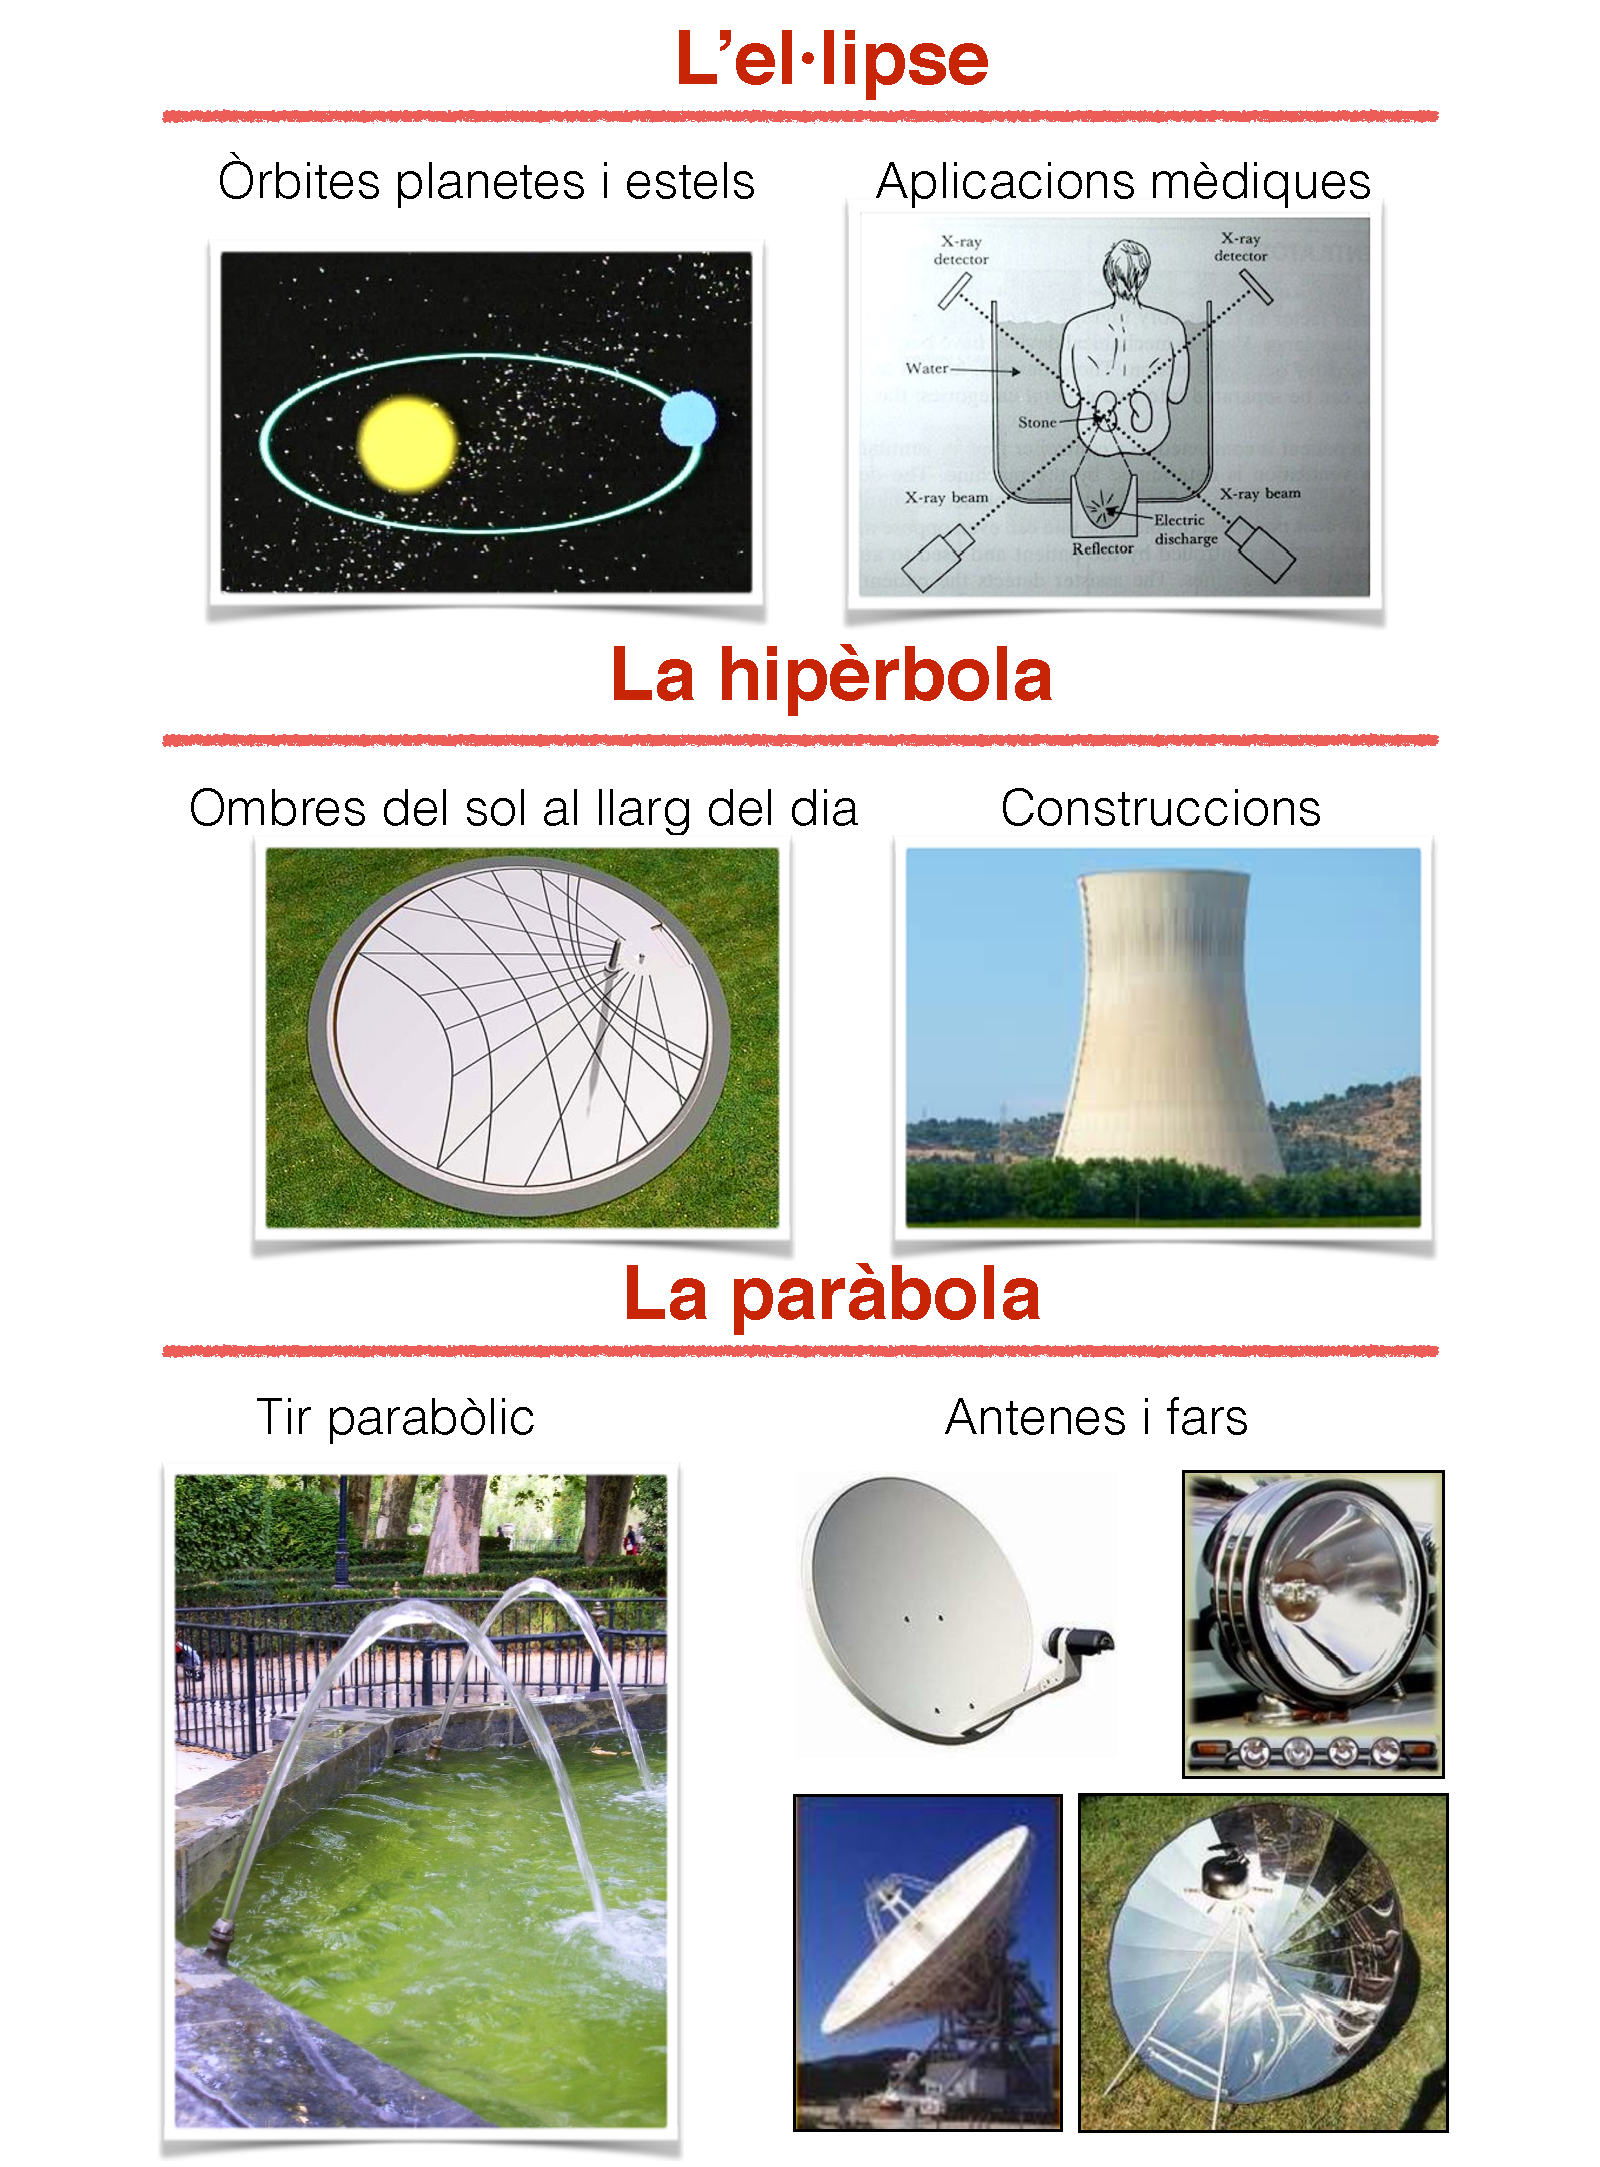
\includegraphics[width=0.95\textwidth]{img-sol/infografia-coniques}
	\end{center}

	\vspace*{\fill}
}


\newcommand{\pagexv}{
	\heading{Intervals i semirectes}

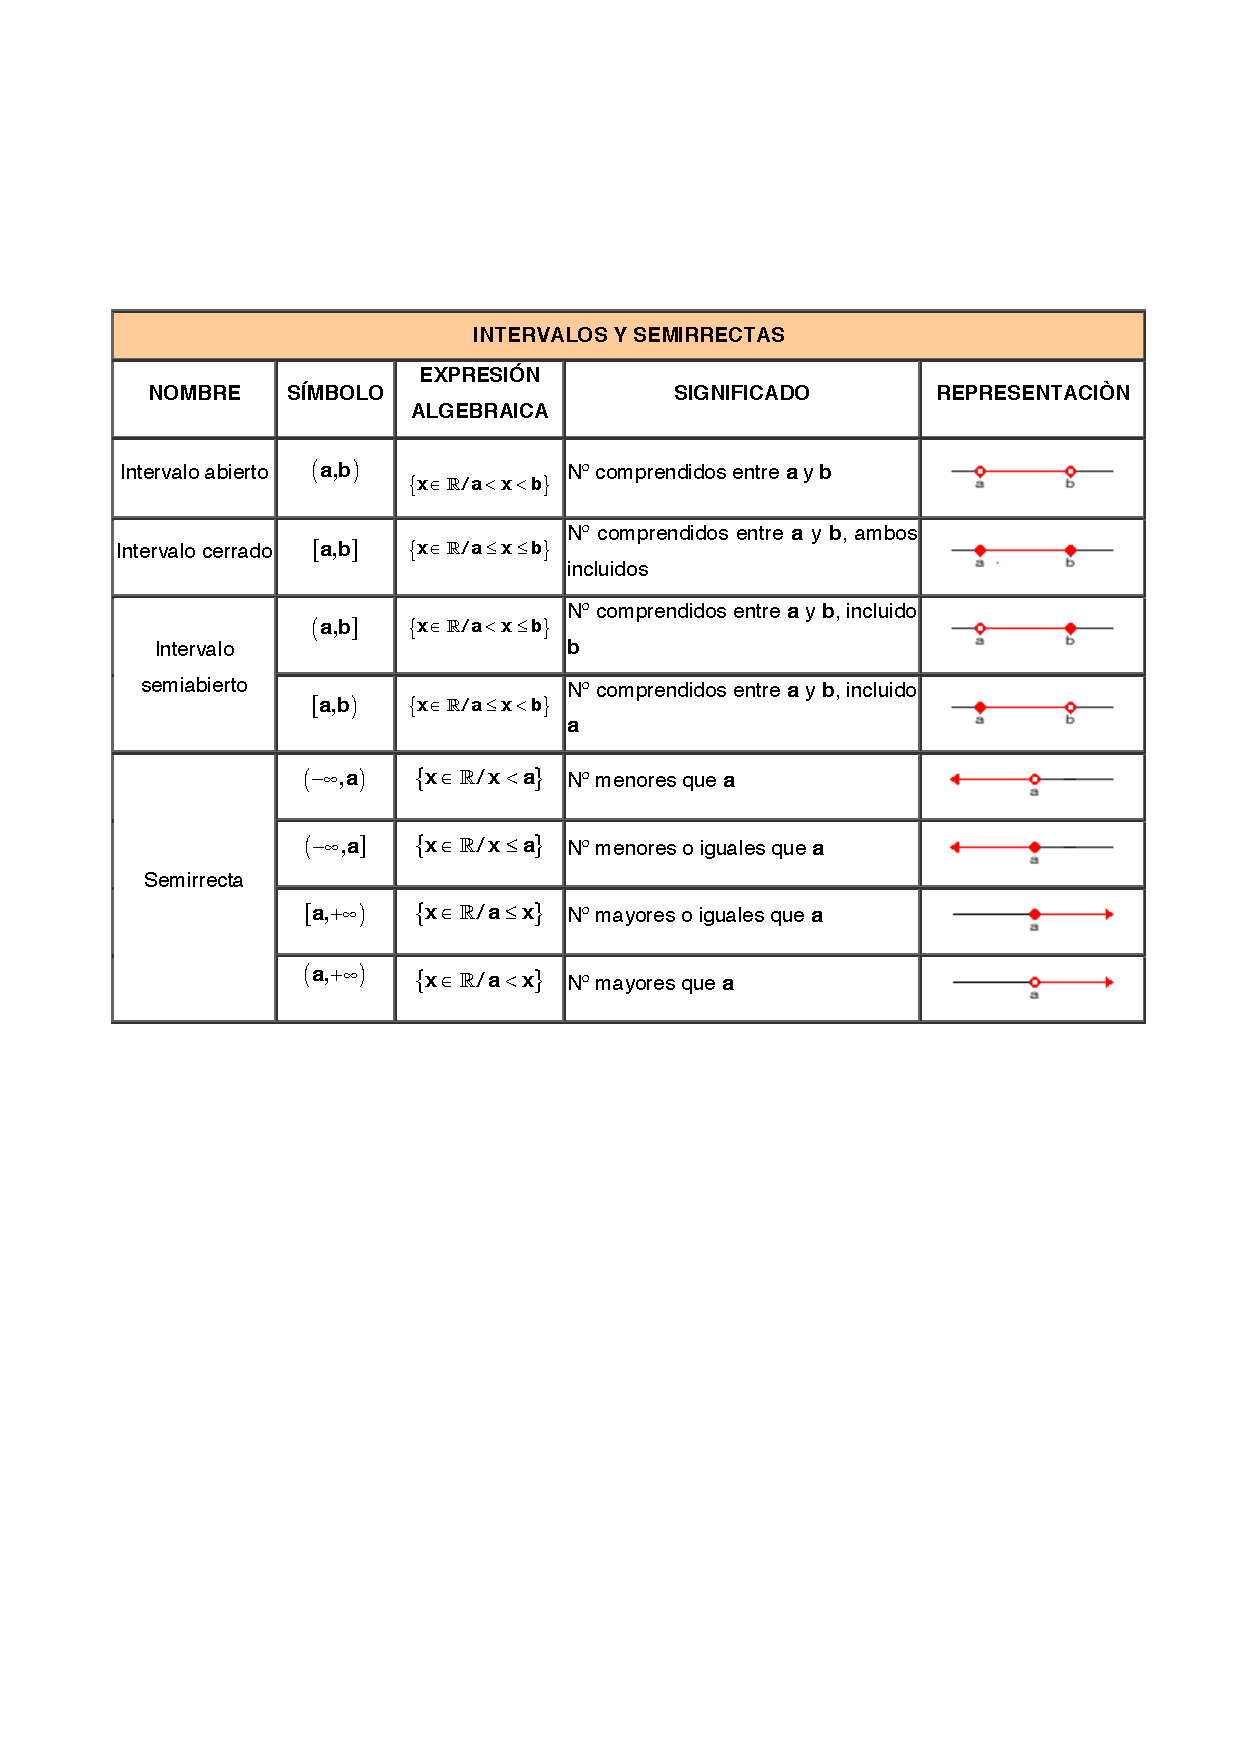
\includegraphics[width=\textwidth]{img-sol/p15-extra}
}

\newcommand{\pagexxix}{
	\heading{Exemples de resolució pel mètode de Gauss}
	
	\subsection*{Sistema Compatible determinat}
	
	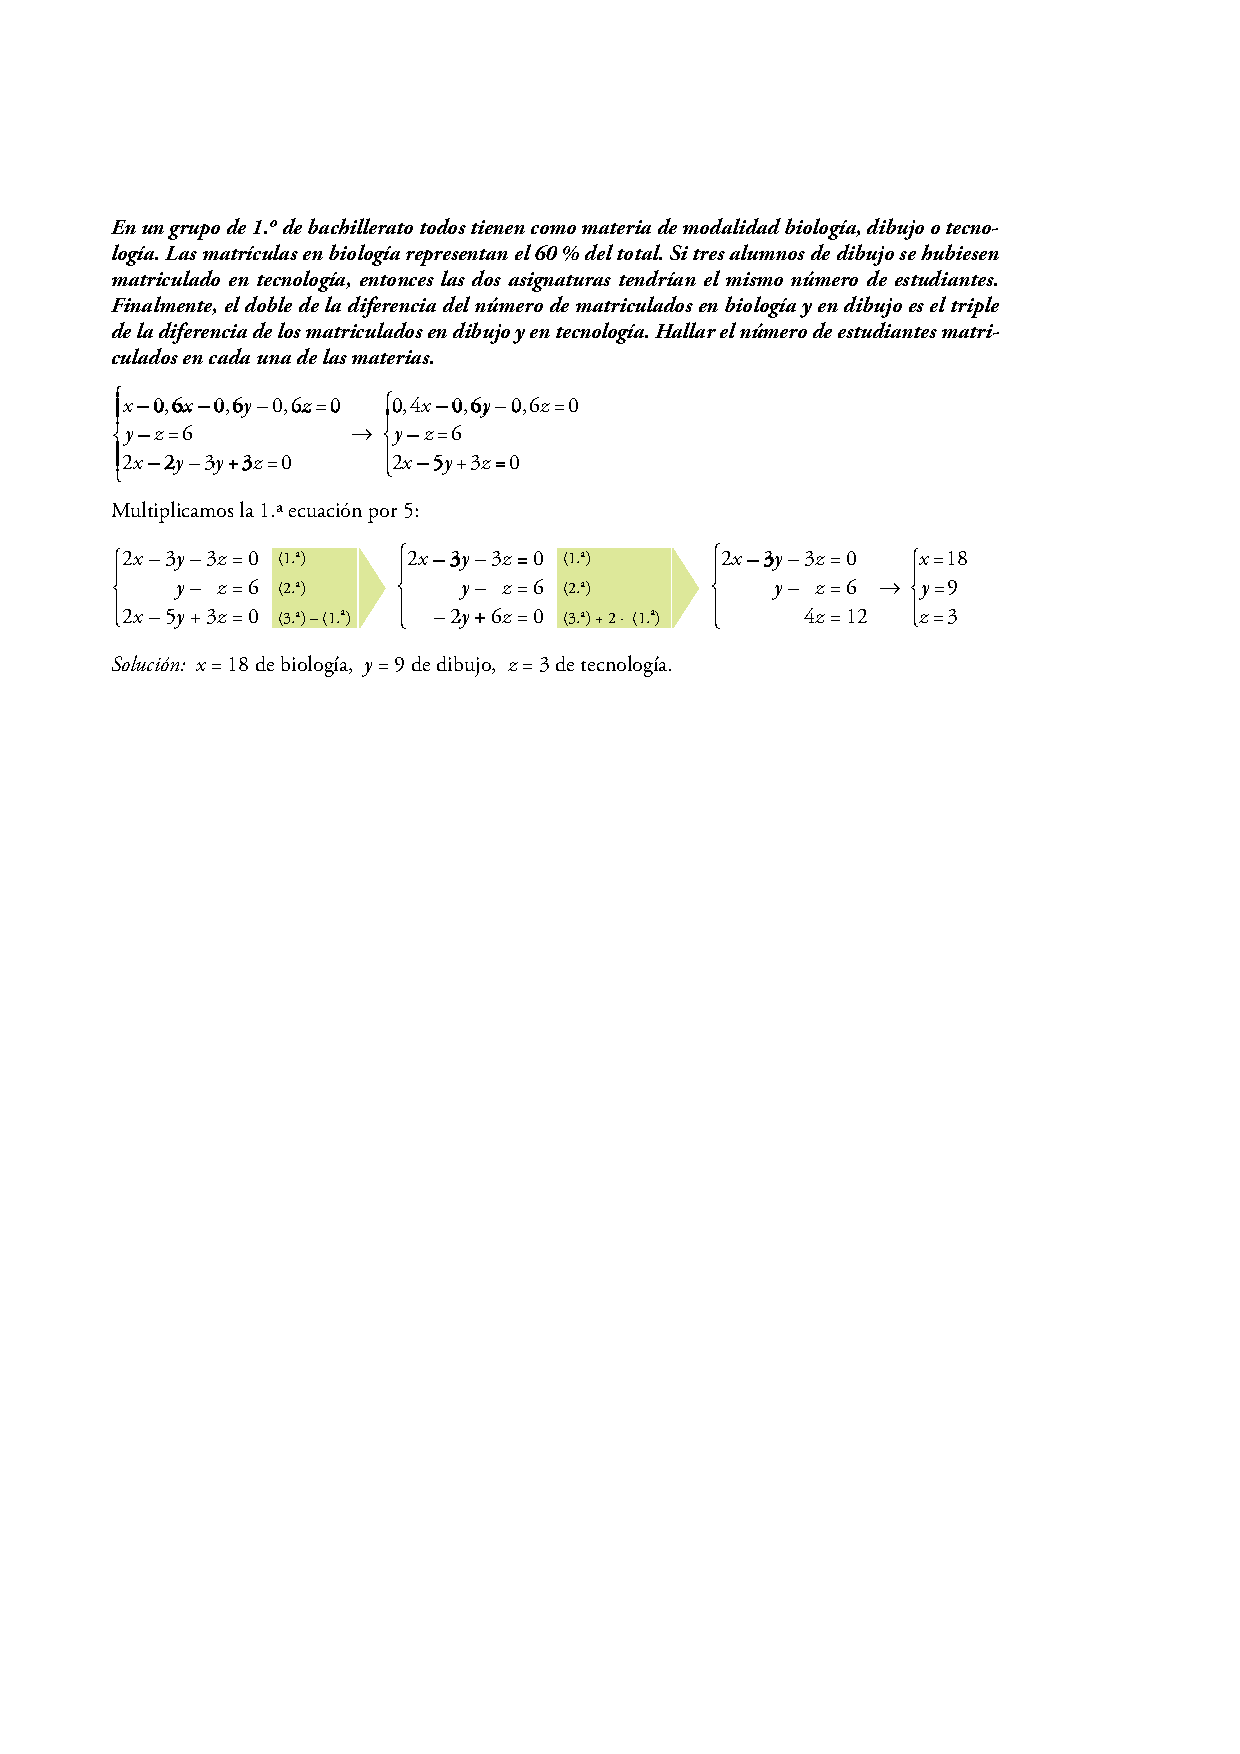
\includegraphics[width=\textwidth]{img-sol/p29-extra1}
	
	\hrule
	
	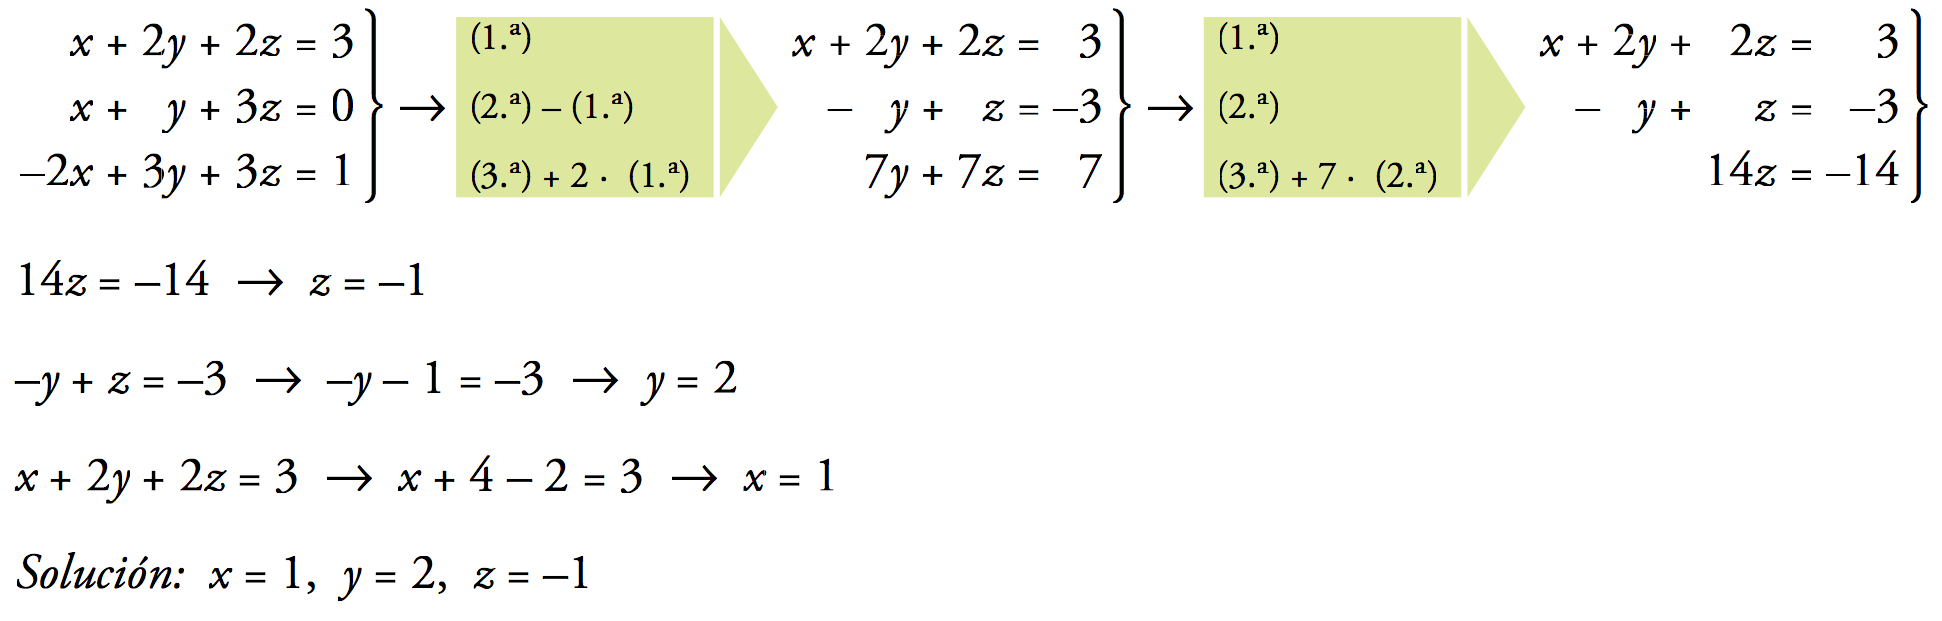
\includegraphics[width=\textwidth]{img-sol/p29-extra2}

	\subsection*{Sistema Compatible indeterminat}
	
	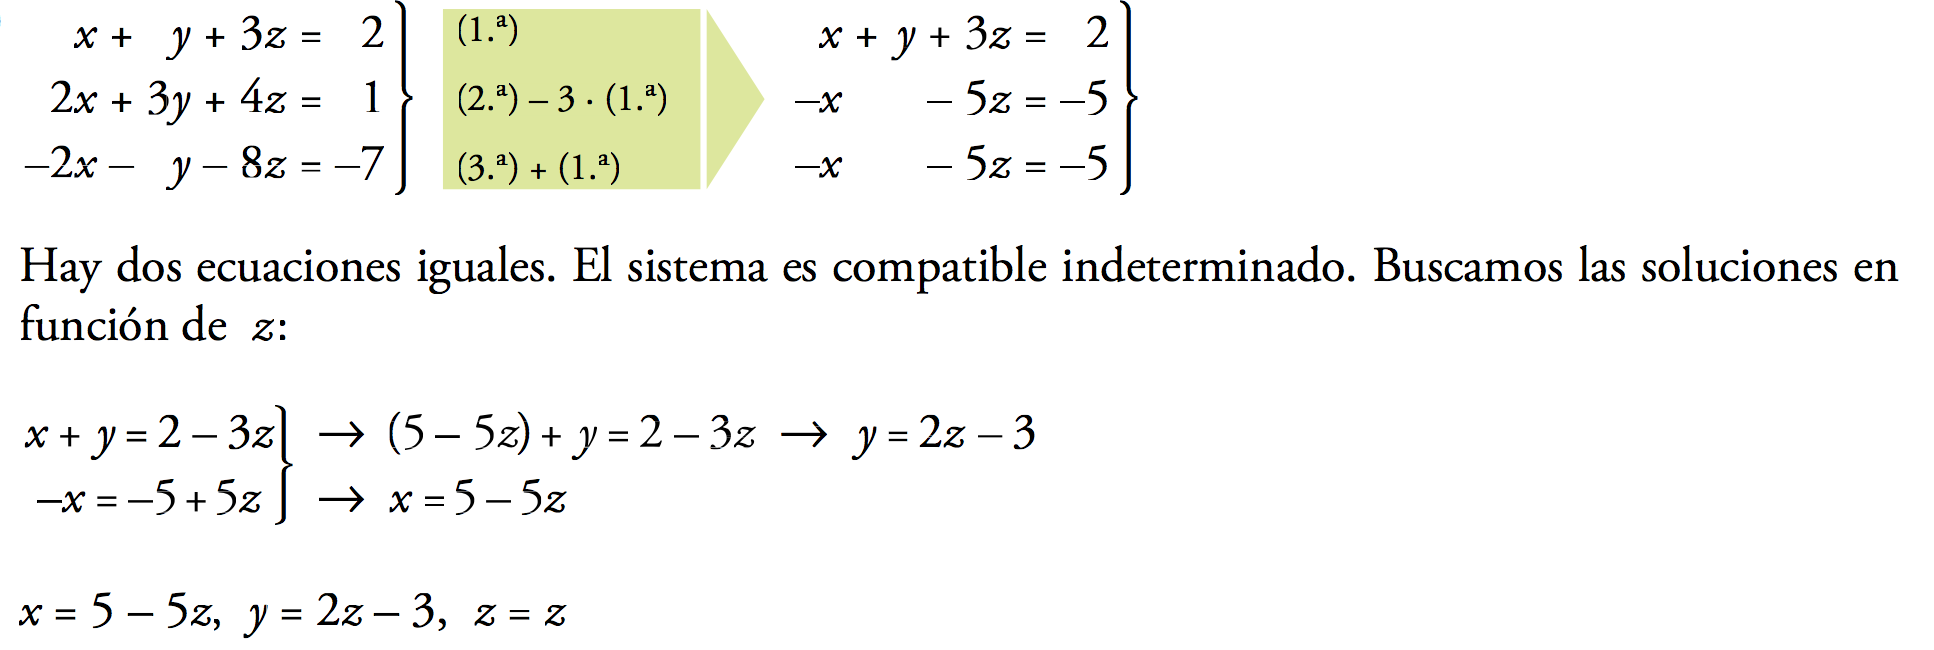
\includegraphics[width=\textwidth]{img-sol/p29-extra3}
}

\newcommand{\pagexxx}{
	\heading{Raons d'angles majors que 90$^\circ$}
 
	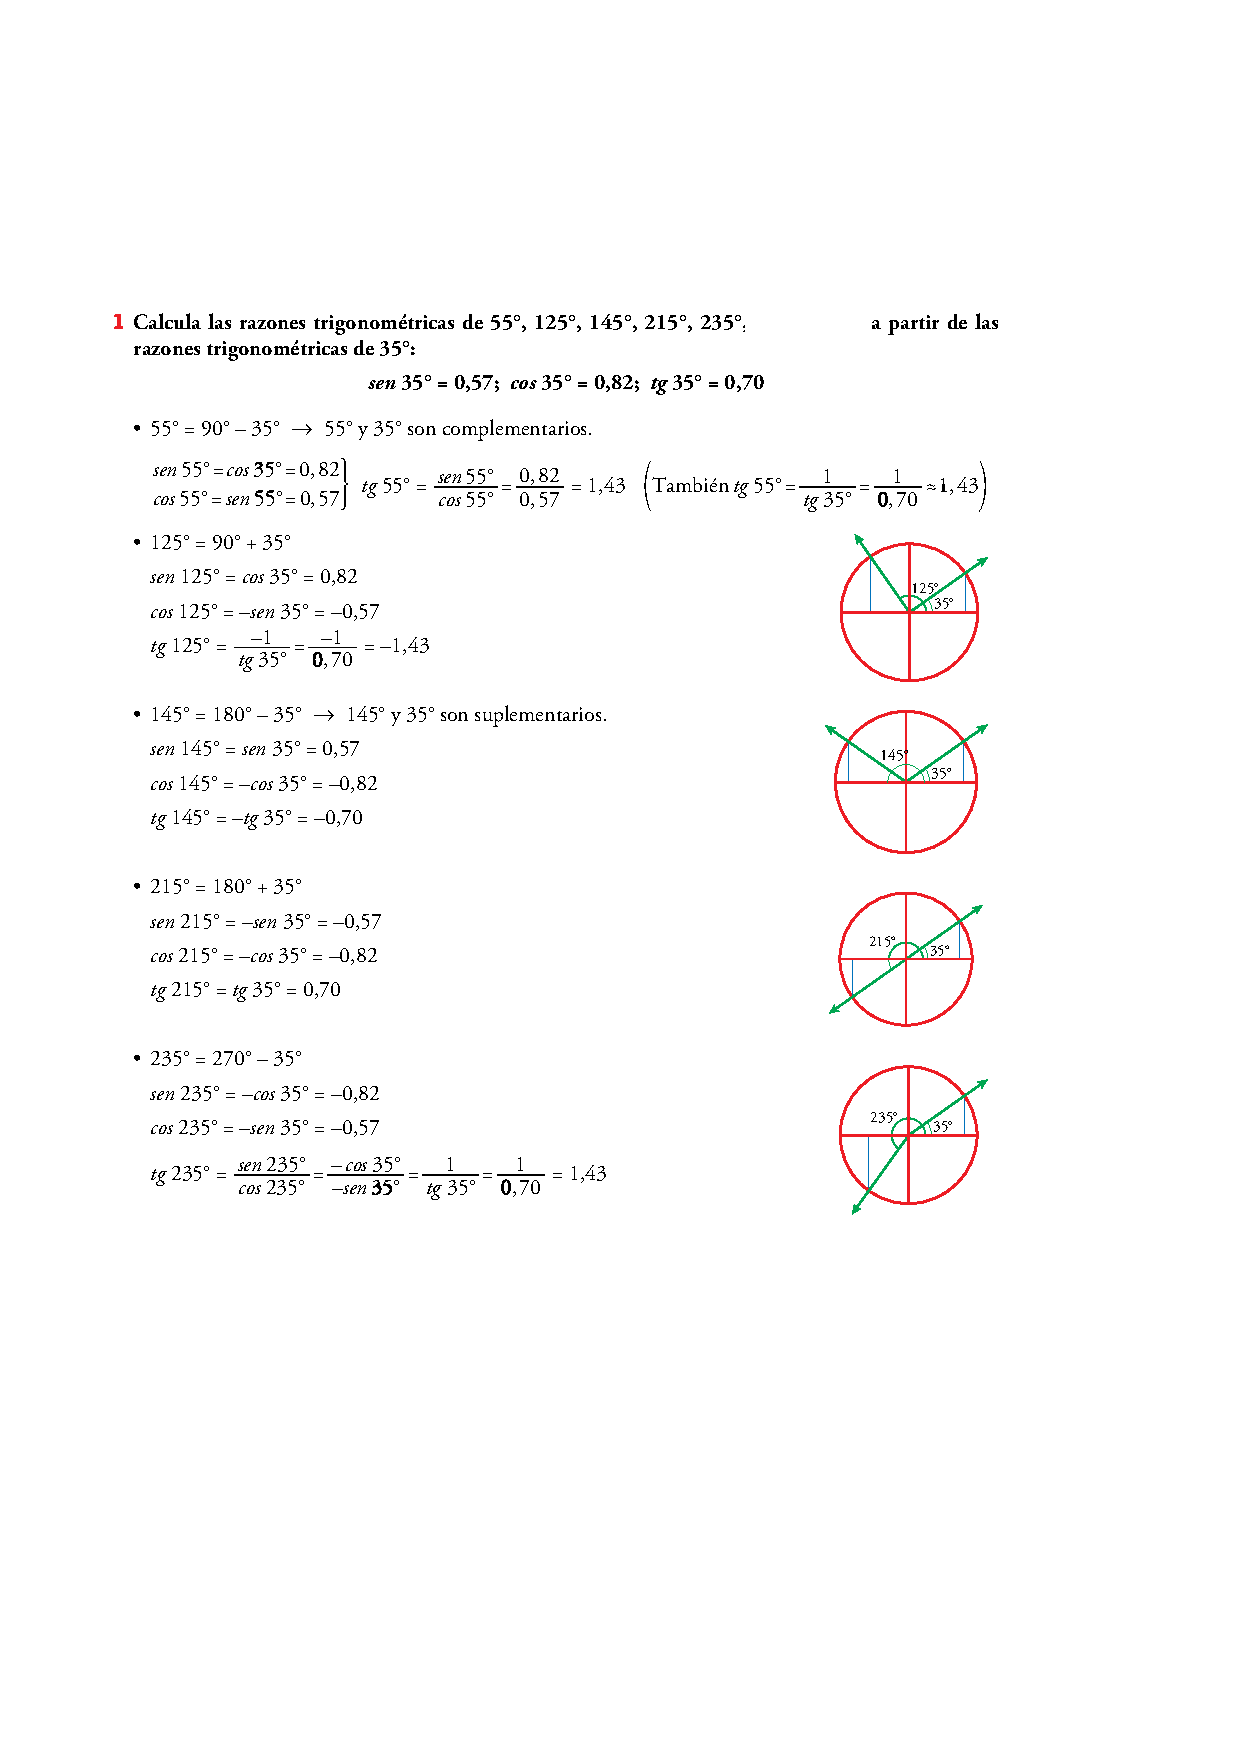
\includegraphics[width=\textwidth]{img-sol/p30-extra1}	
}


\newcommand{\pagexlvii}{
	\heading{Representació dels nombres complexos}
\begin{center}
	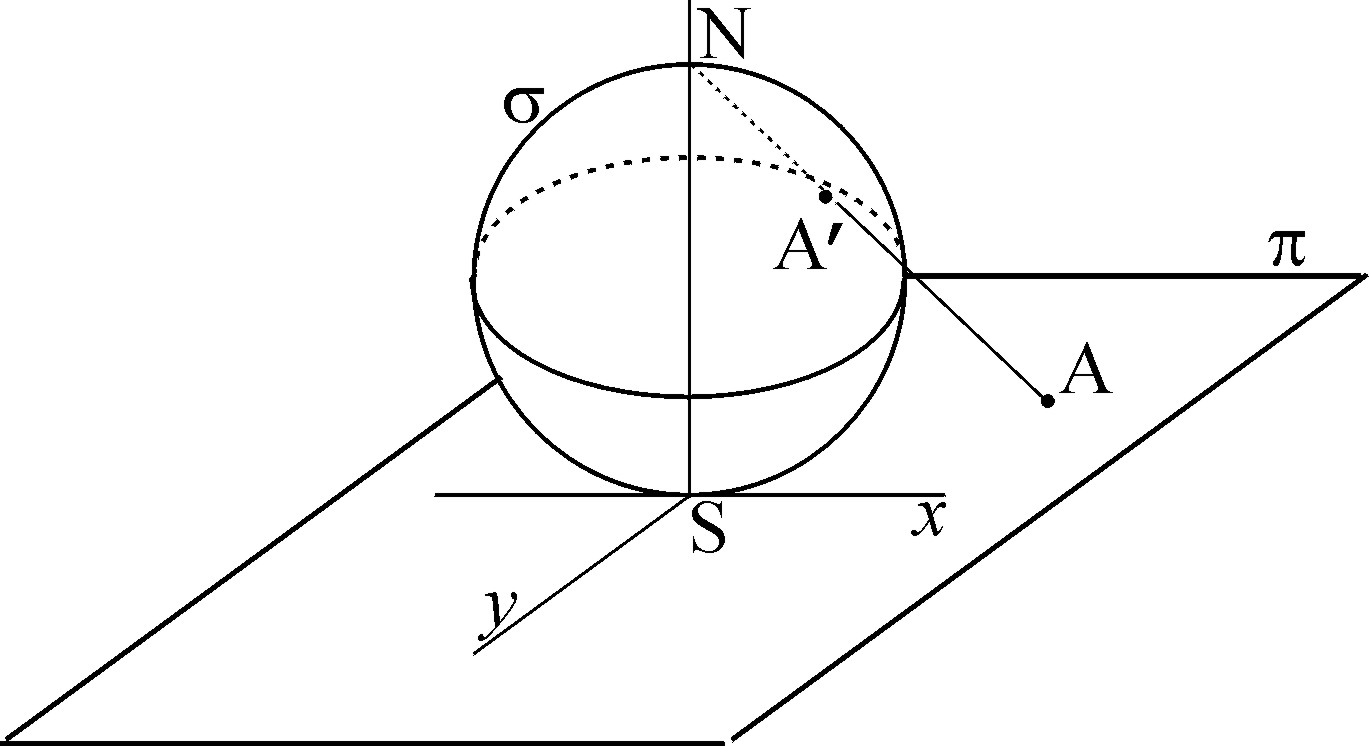
\includegraphics[width=0.5\textwidth]{img-sol/p47-extra1}
\end{center}

\vso 

\heading{Objectius del tema:}

\vspace{0.25cm}
{
	\fontsize{10.5}{12.8}\selectfont
	2. Conèixer els nombres complexos com a extensió dels nombres reals, utilitzant-los per obtenir solucions d’algunes equacions algebraiques.
	
	2.1. Valora els nombres complexos com a ampliació del concepte de nombre real i els utilitza per obtenir la solució d’equacions de segon grau amb coeficients reals sense solució real.
	
	2.2. Opera amb nombres complexos, i els representa gràficament, i utilitza la fórmula de Moivre en el cas de les potències
}

%%%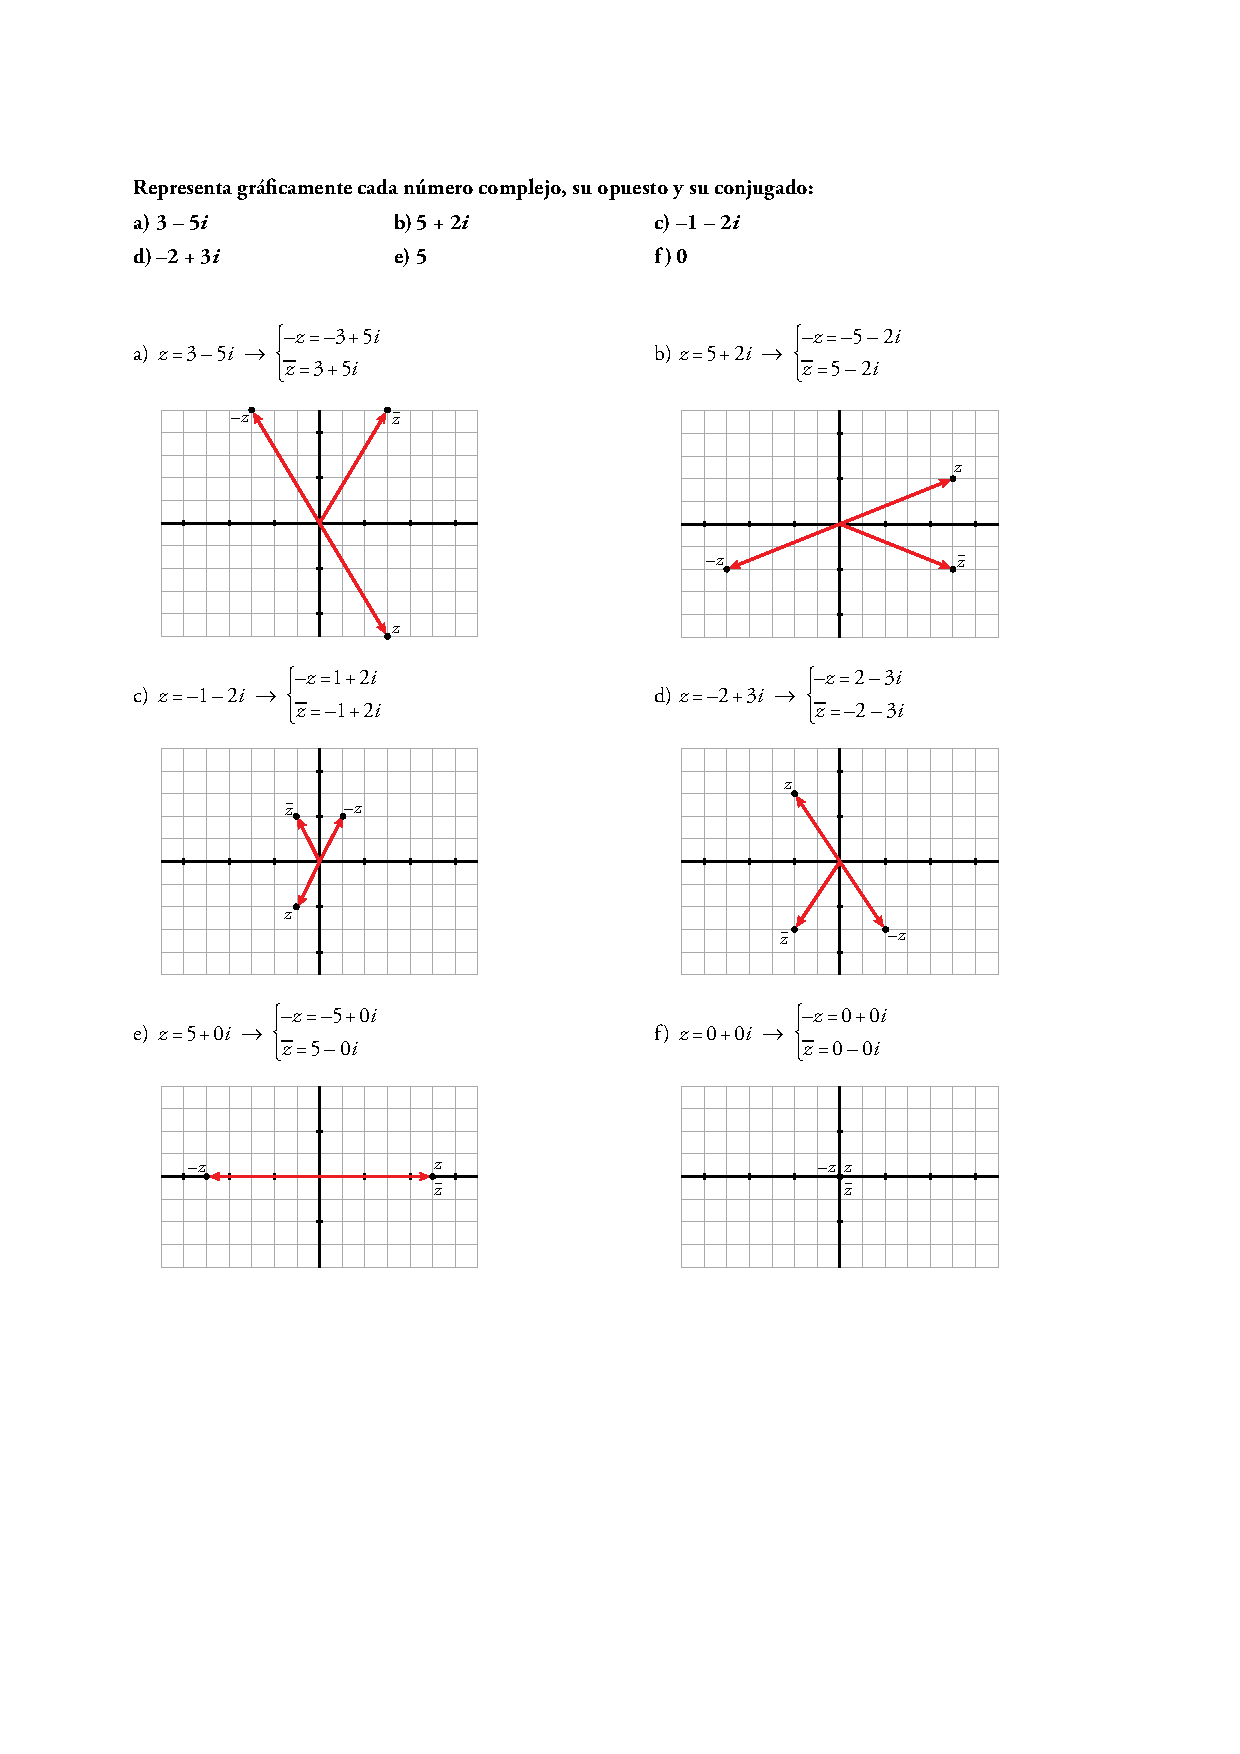
\includegraphics[width=\textwidth]{img-sol/p47-extra2}
}

\newcommand{\pagelxxii}{
\heading{Concepte de límit}

\subsection*{A partir d'una gràfica}
\begin{center}
	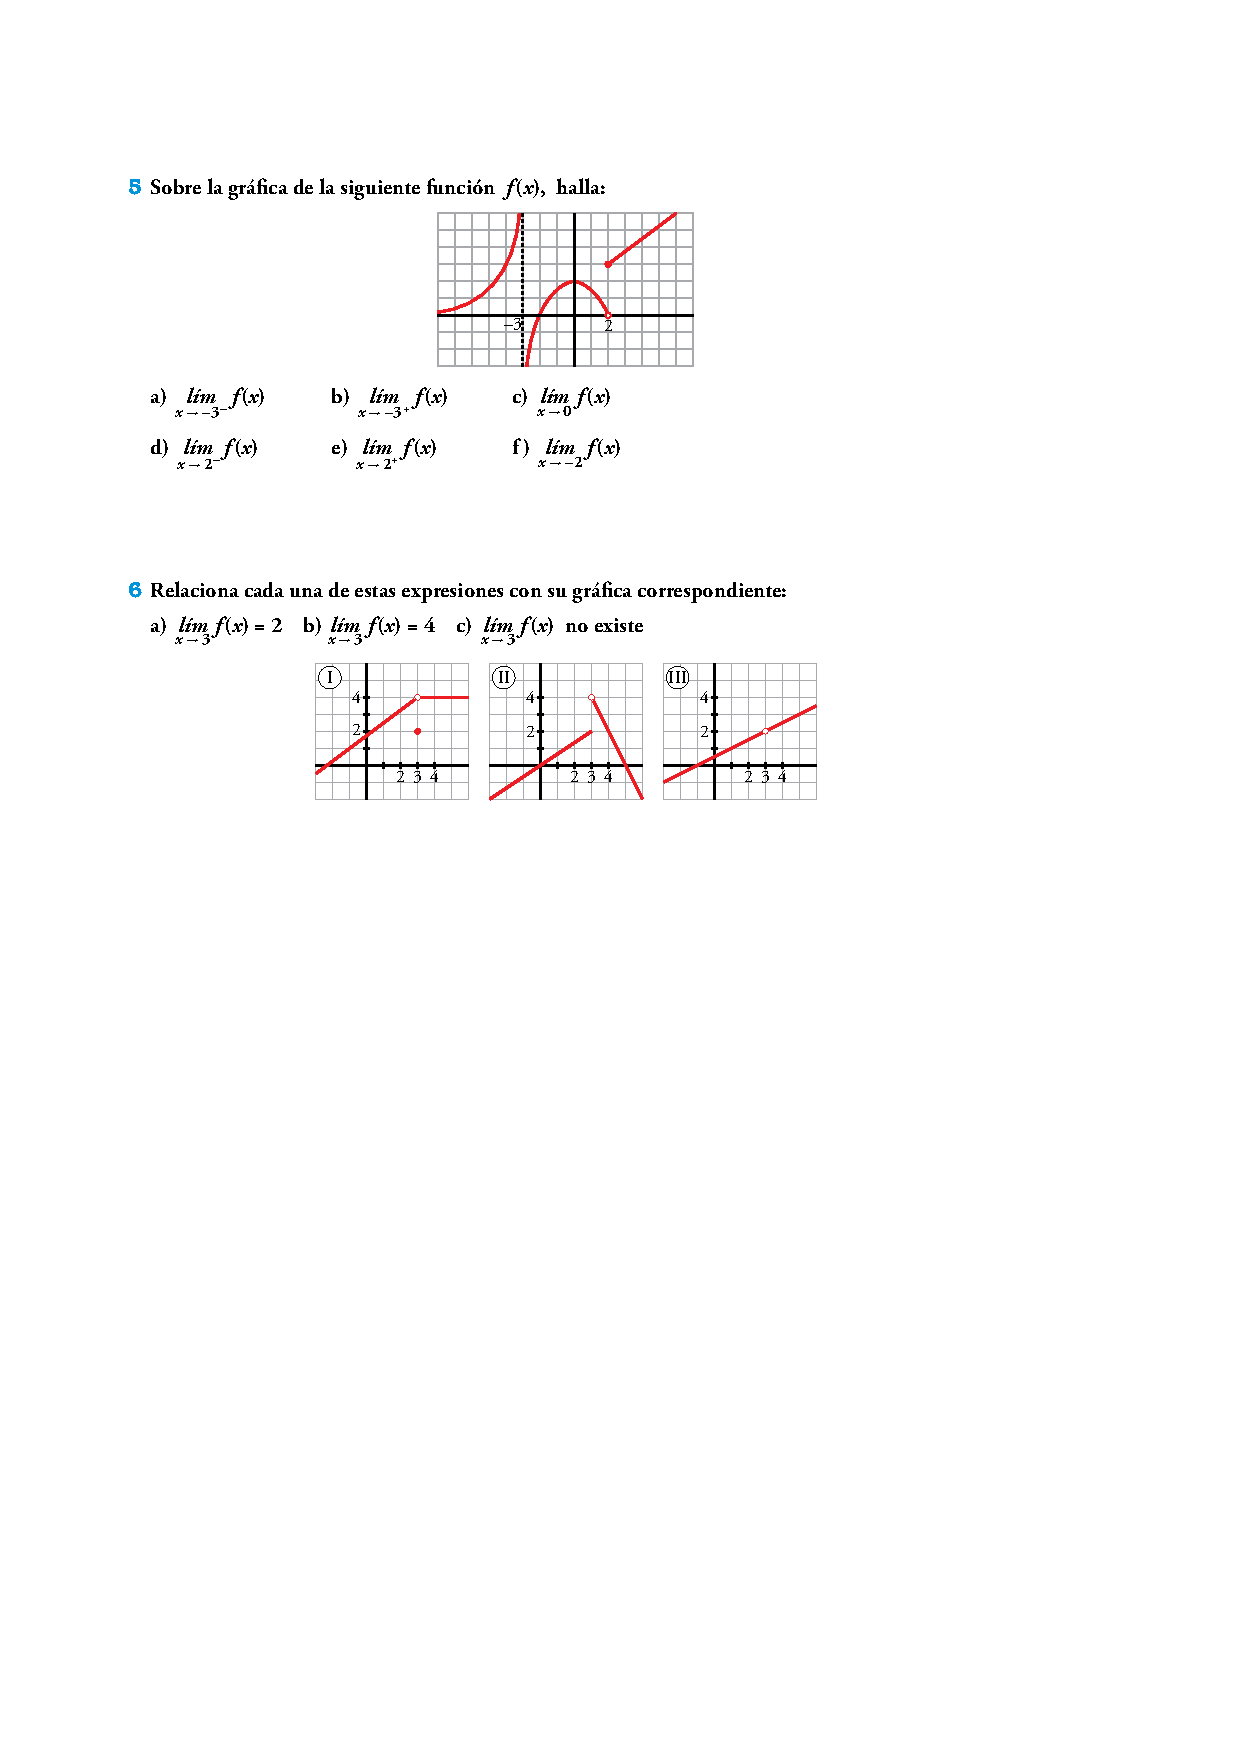
\includegraphics[width=\textwidth]{img-sol/p72-extra1}
\end{center}


\subsection*{A partir d'una taula de valors}

\begin{multicols}{2}
\begin{center}
	\[ f(x)= \dfrac{\sqrt{x}-1}{x^2-1} \]
 \begin{tabular}{|c|c|}\hline
 	$x$ & $y$ \\\hline
 	0.9 & 0.270088\\\hline
 	0.99 & 0.251888\\\hline
 	0.999 & 0.2501876\\\hline
 	0.9999 & 0.2500187\\\hline
 \end{tabular}
\[ \limx{1^-} \dfrac{\sqrt{x}-1}{x^2-1}=0.25=\dfrac{1}{4}\]
\columnbreak
	\[ f(x)= \dfrac{2x+1}{\sqrt{x}} \]
\begin{tabular}{|c|c|}\hline
	$x$ & $y$ \\\hline
	10 & 6.641 \\\hline
	1000 & 63.277 \\\hline
	1000000 & 2000.001 \\\hline
	100000000 & 20000.001 \\\hline
\end{tabular}
\[ \limx{+\infty} \dfrac{2x+1}{\sqrt{x}}=+\infty\]

\end{center}
\end{multicols}
}

\newcommand{\pagelviii}{
	\vspace*{\fill}
	\begin{center}
		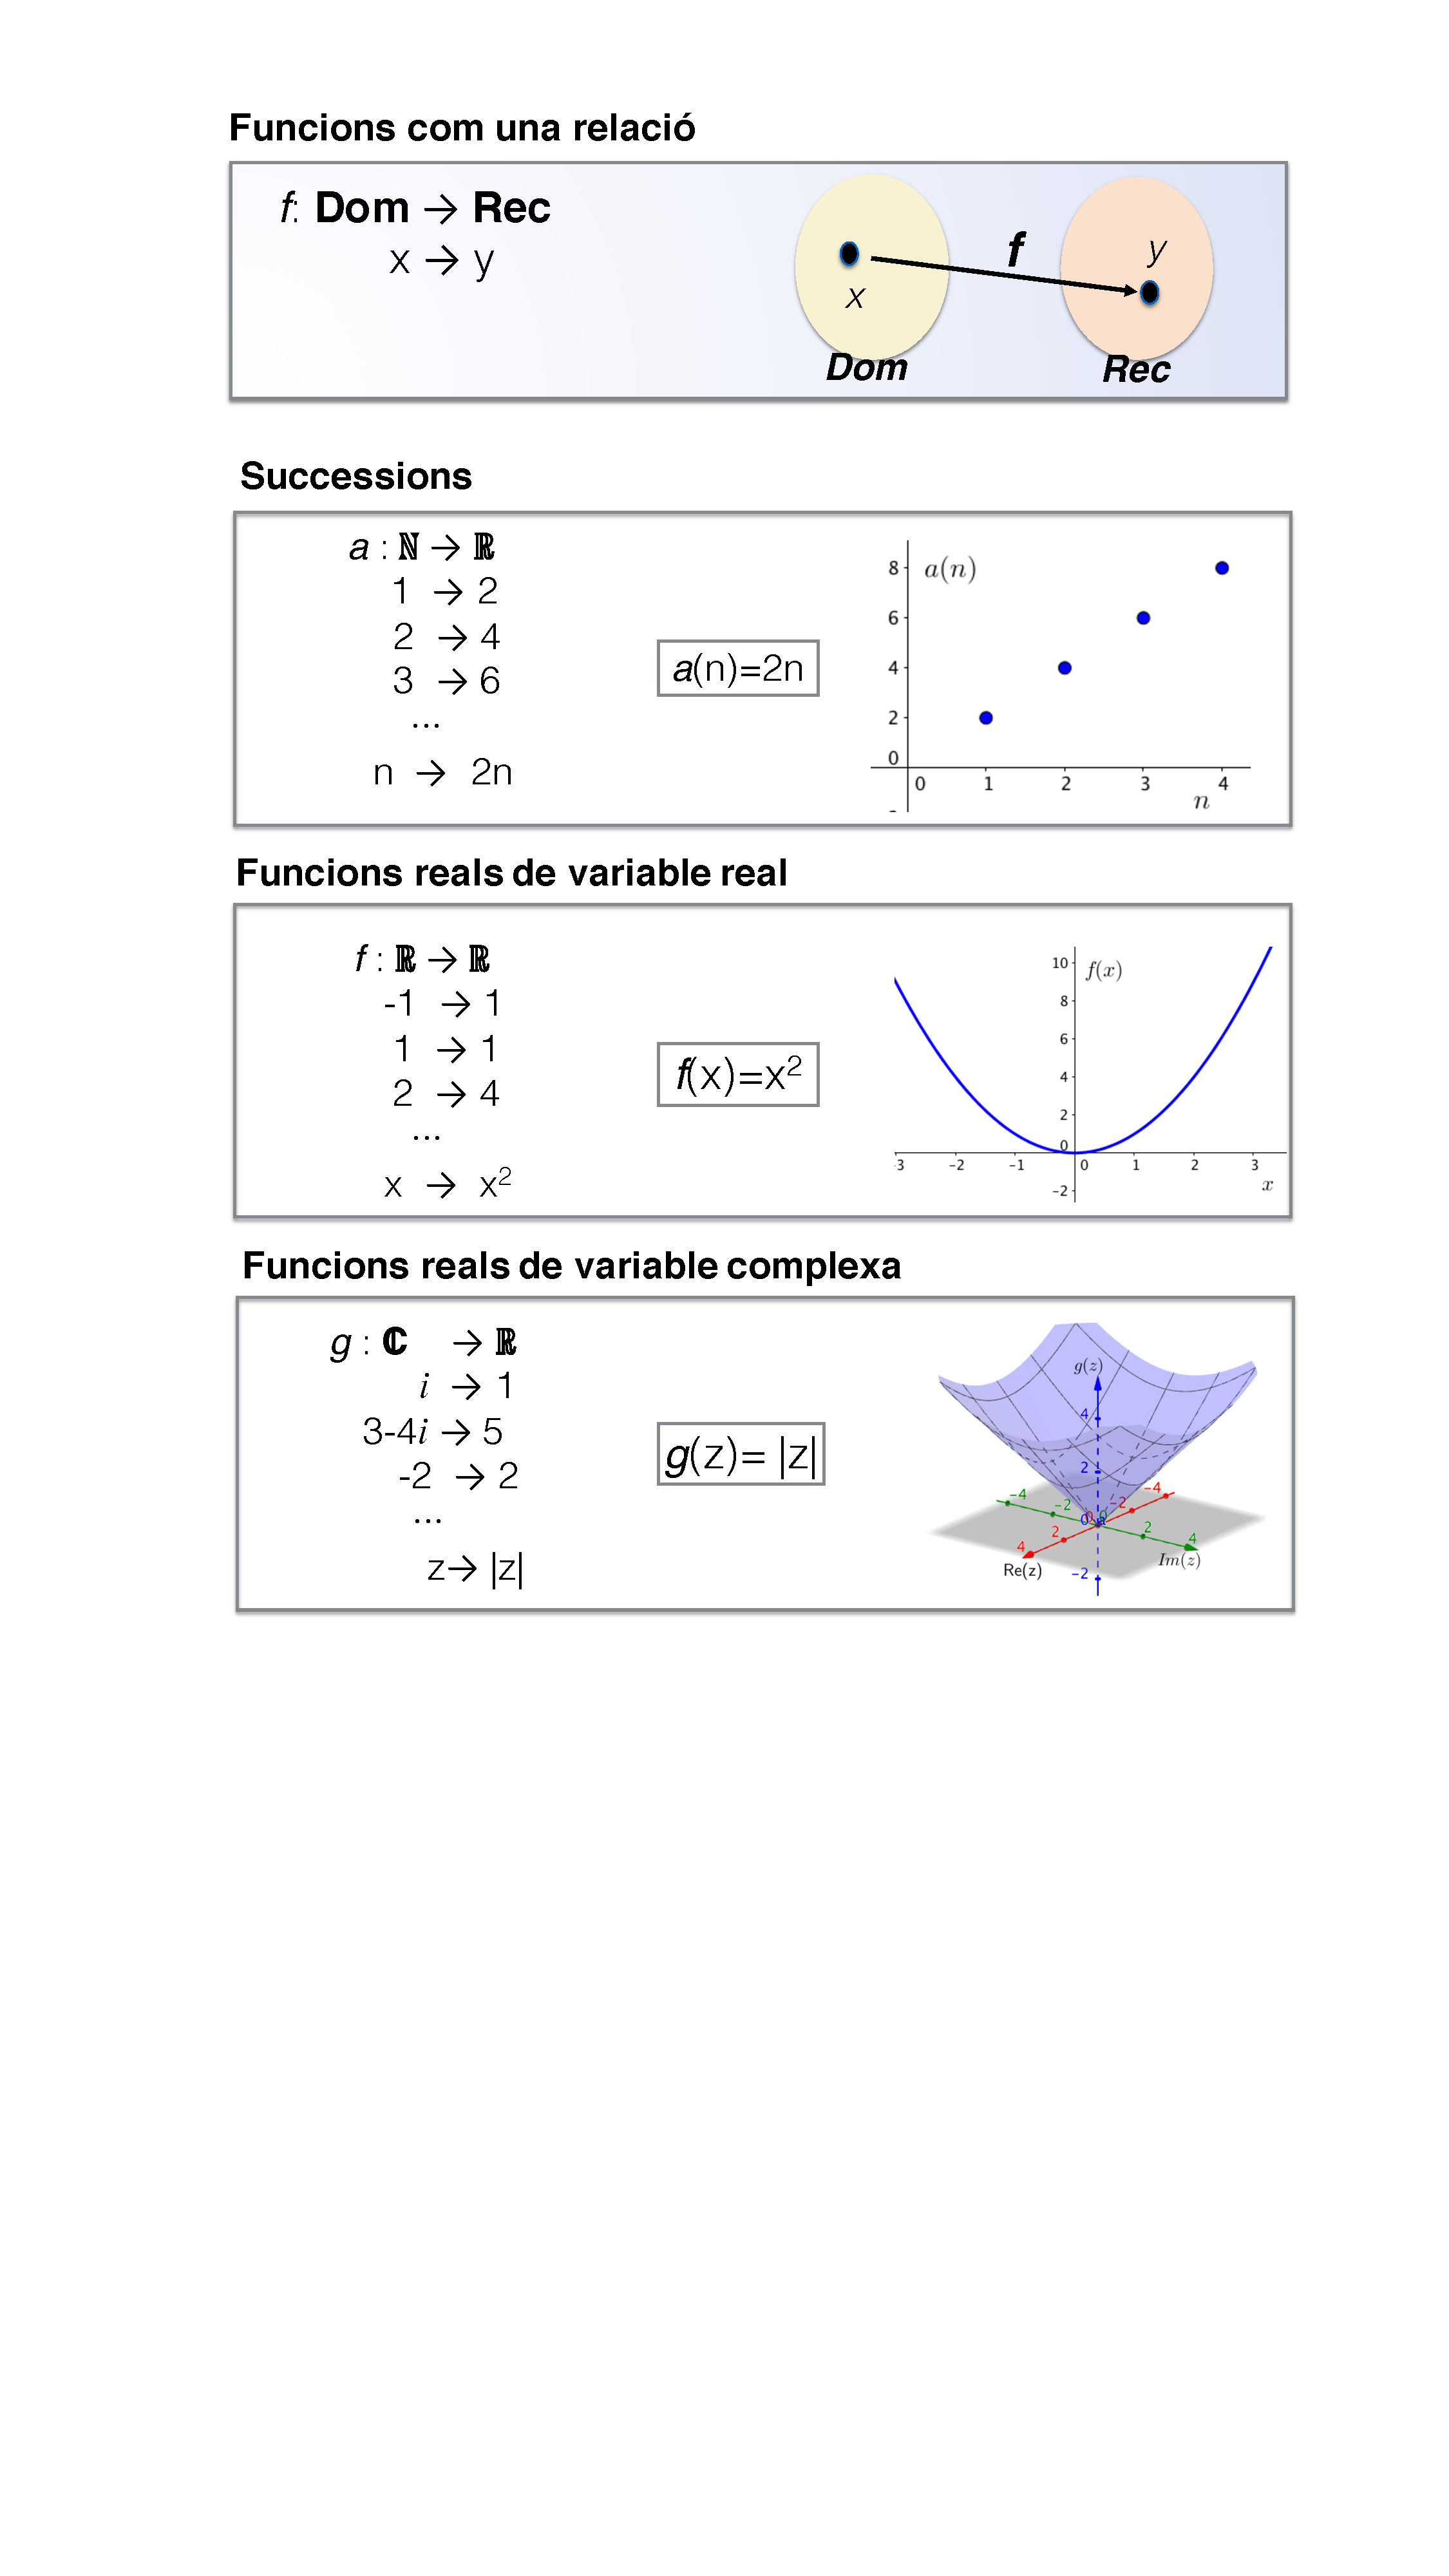
\includegraphics[width=0.8\textwidth]{img-sol/p58-extra1}
	\end{center}
	\vspace*{\fill}
}
 

\newcommand{\pagelxxv}{
\heading{Exemple càlcul de límits amb radicals}

\vso

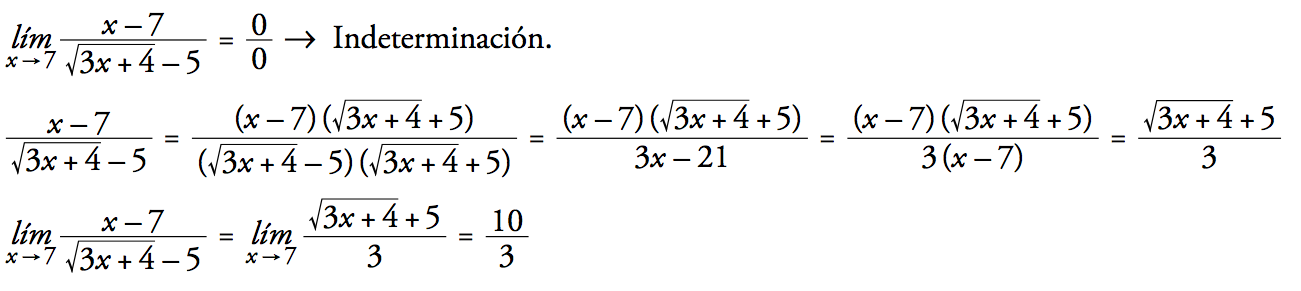
\includegraphics[width=\textwidth]{img-sol/p75-extra1}

\vso
\hrule
\vso

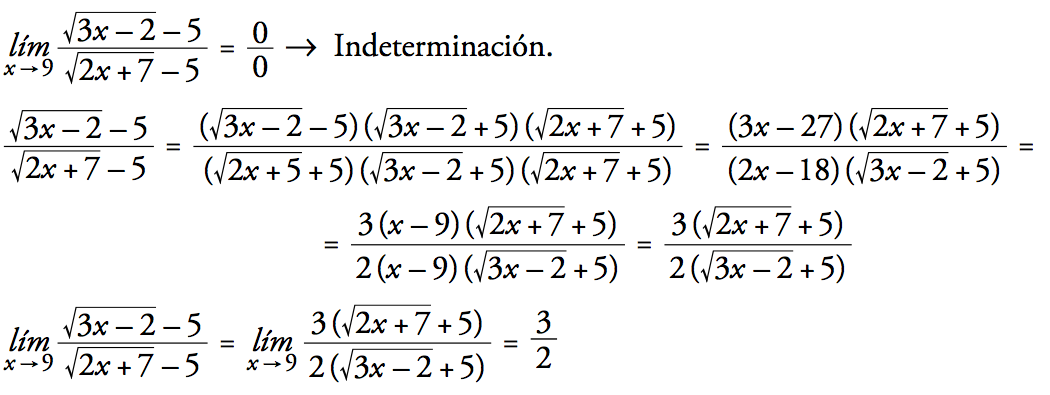
\includegraphics[width=\textwidth]{img-sol/p75-extra2}
}

\newcommand{\pagelxxix}{
\textbf{\large $\bullet$ Gràfics Ex. 14:}

\begin{center}
a) 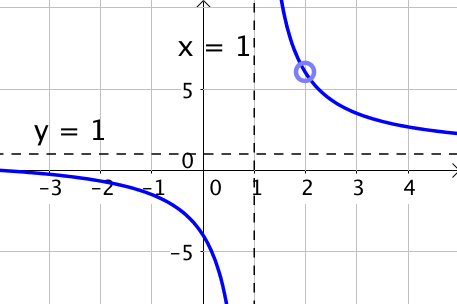
\includegraphics[width=0.38\textwidth]{img-sol/p79-extra-a}
b) 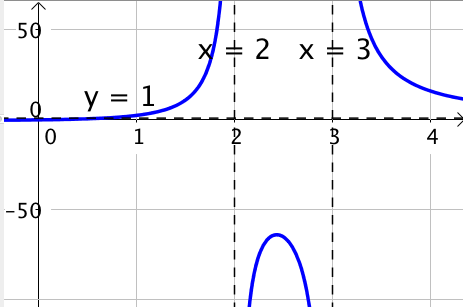
\includegraphics[width=0.38\textwidth]{img-sol/p79-extra-b}

c) 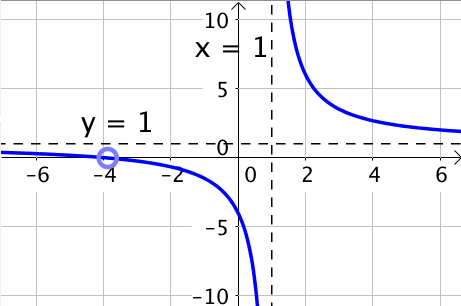
\includegraphics[width=0.38\textwidth]{img-sol/p79-extra-c}
d) 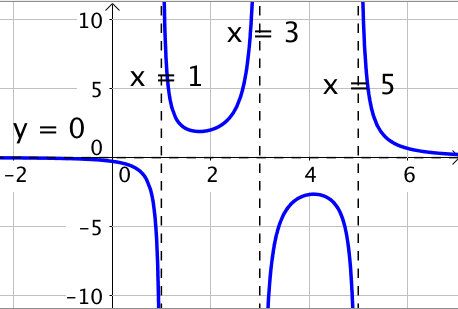
\includegraphics[width=0.38\textwidth]{img-sol/p79-extra-d}
\end{center}
}


\newcommand{\pagelxxx}{
	\textbf{\large $\bullet$ Gràfics Ex. 16:}
	
	\begin{center}
		a) 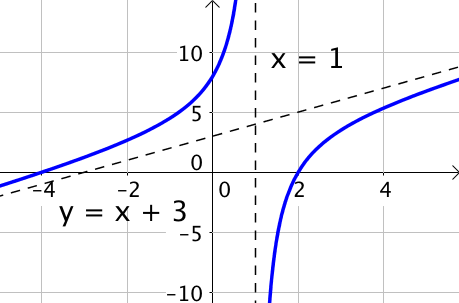
\includegraphics[width=0.38\textwidth]{img-sol/p80-extra-a}
		b) 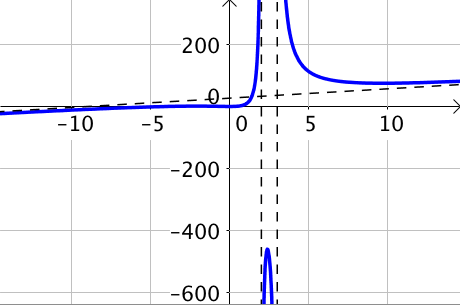
\includegraphics[width=0.38\textwidth]{img-sol/p80-extra-b}
		
		c) 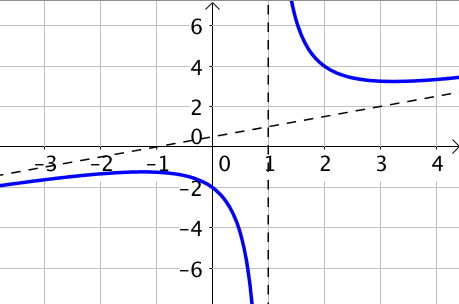
\includegraphics[width=0.38\textwidth]{img-sol/p80-extra-c}
		d) 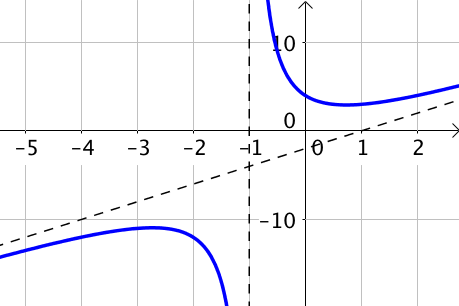
\includegraphics[width=0.38\textwidth]{img-sol/p80-extra-d}
	\end{center}
}


\newcommand{\pagelxxxi}{
	\textbf{\large $\bullet$ Gràfics Ex. 19:}
	
	\begin{center}
		a) 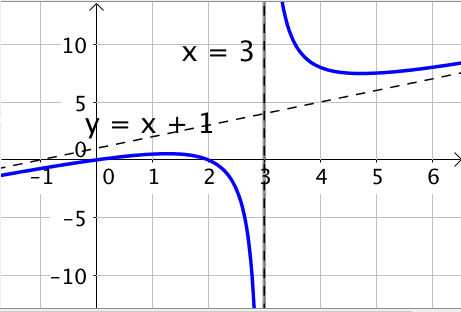
\includegraphics[width=0.35\textwidth]{img-sol/p81-extra-a}
		b) 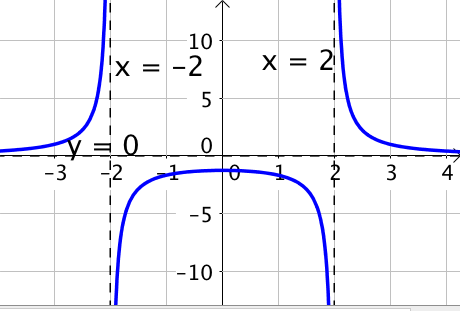
\includegraphics[width=0.35\textwidth]{img-sol/p81-extra-b}
		
		c) 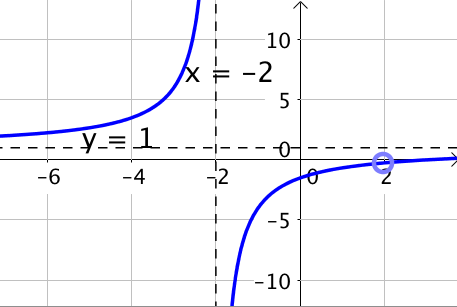
\includegraphics[width=0.35\textwidth]{img-sol/p81-extra-c}
		d) 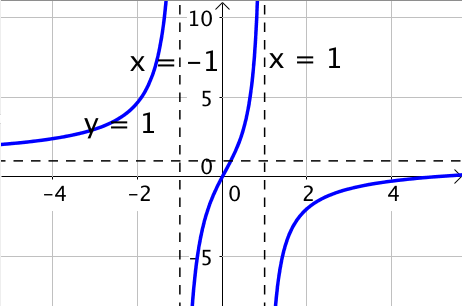
\includegraphics[width=0.35\textwidth]{img-sol/p81-extra-d}
		
		e) 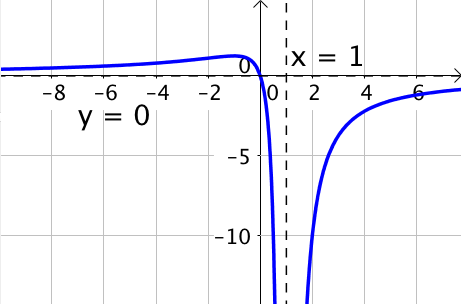
\includegraphics[width=0.35\textwidth]{img-sol/p81-extra-e}
		f) 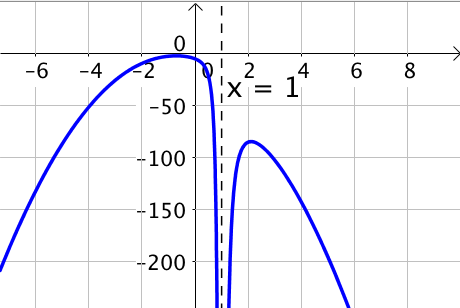
\includegraphics[width=0.35\textwidth]{img-sol/p81-extra-f}
		
		g) 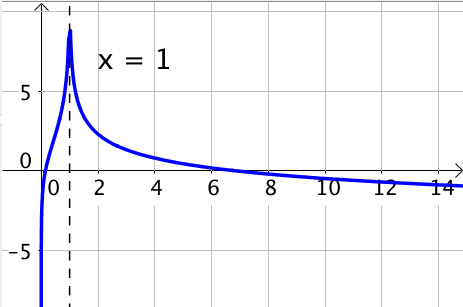
\includegraphics[width=0.35\textwidth]{img-sol/p81-extra-g}
		h) 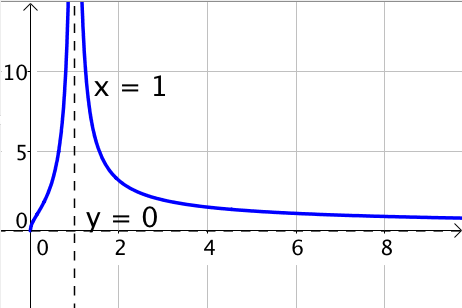
\includegraphics[width=0.35\textwidth]{img-sol/p81-extra-h}
	\end{center}
}

\newcommand{\pagecii}{
\newpage

\heading{Exemples de problemes d'optimització}

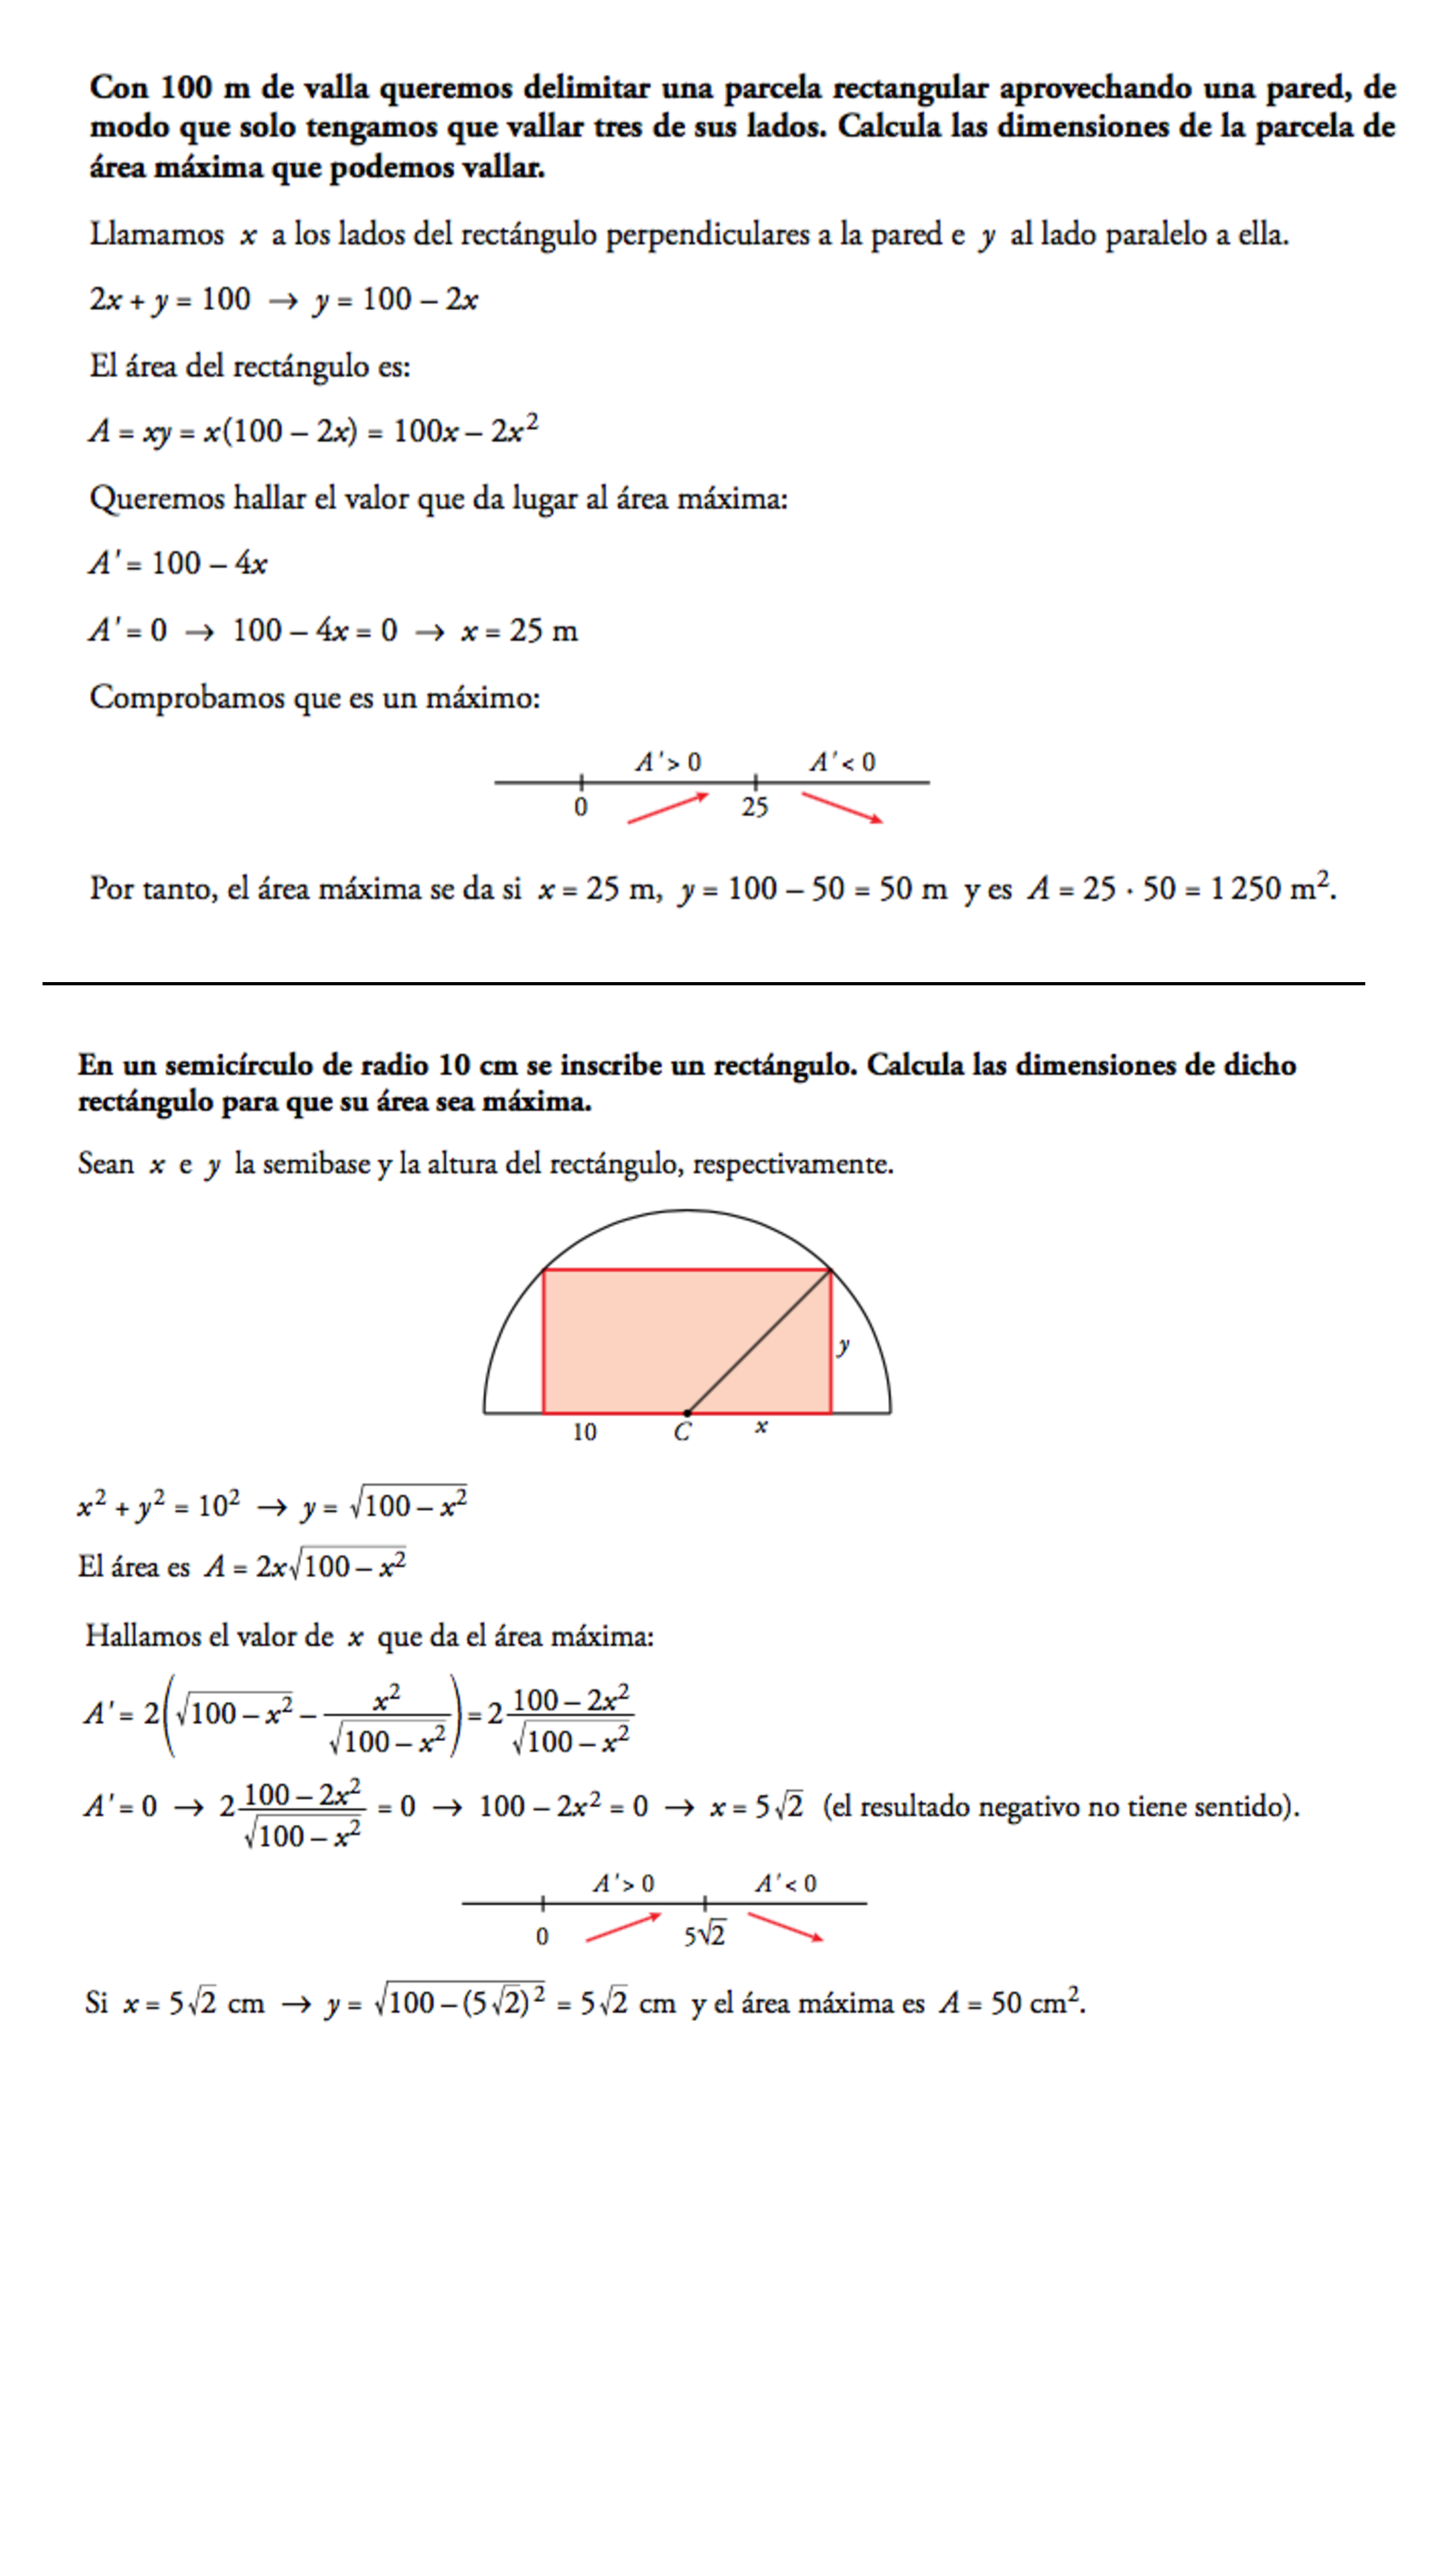
\includegraphics[width=0.95\textwidth]{img-sol/p99-extra}
}


\newcommand{\pagecx}{
\heading{Operacions amb vectors gràficament}

\vso
\begin{center}
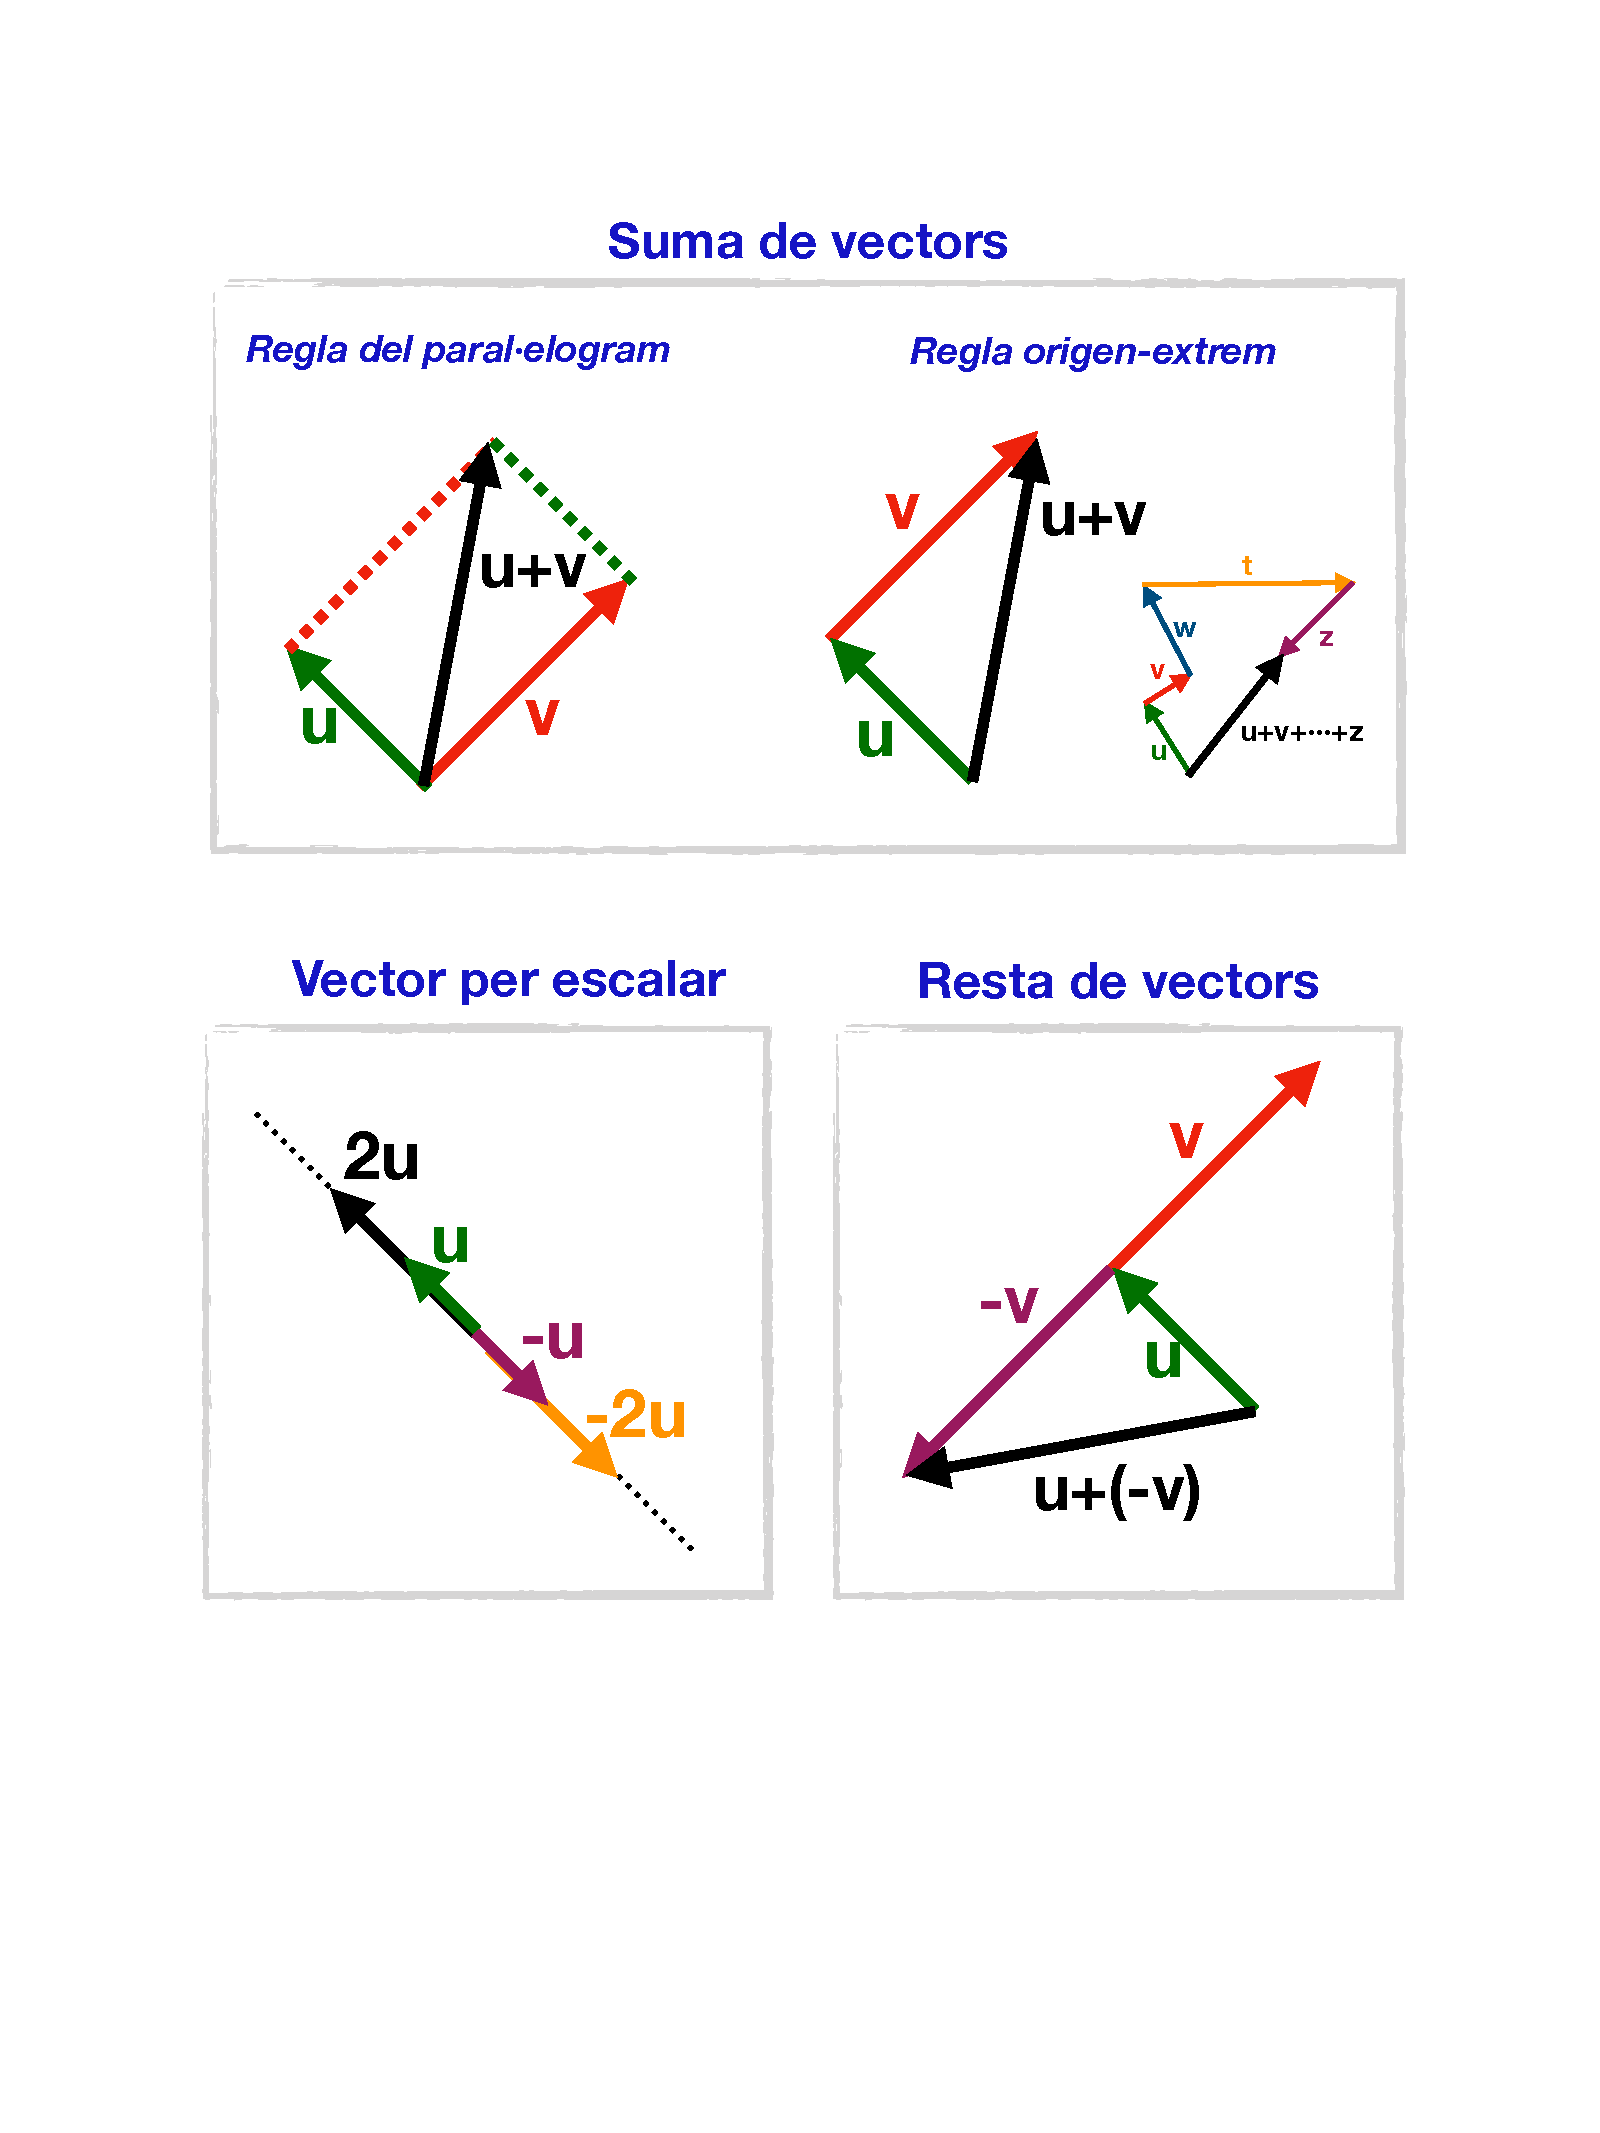
\includegraphics[width=0.75\textwidth]{img-sol/p110-extra}
\end{center}
\vso

\heading{Objectius del tema:}

\vspace{0.25cm}
{
	\fontsize{10.5}{12.8}\selectfont
	 3. Fer servir l’operació del producte escalar i les seves conseqüències. Entendre els conceptes de base ortogonal i ortonormal. Distingir i manejar-se amb precisió en el pla euclidià i en el pla mètric, utilitzant en ambdós casos les seves eines i propietats.
	 
3.1. Empra amb assiduïtat les conseqüències de la definició de producte escalar per normalitzar vectors, calcular el cosinus d’un angle, estudiar l’ortogonalitat de dos vectors o la projecció d’un vector sobre un altre.

3.2. Calcula l’expressió analítica del producte escalar, del mòdul i del cosinus de l’angle.

}
}

\newcommand{\pagecxxiv}{
	\heading{Demostració fórmula distància punt -- recta}
	
	\begin{center}
		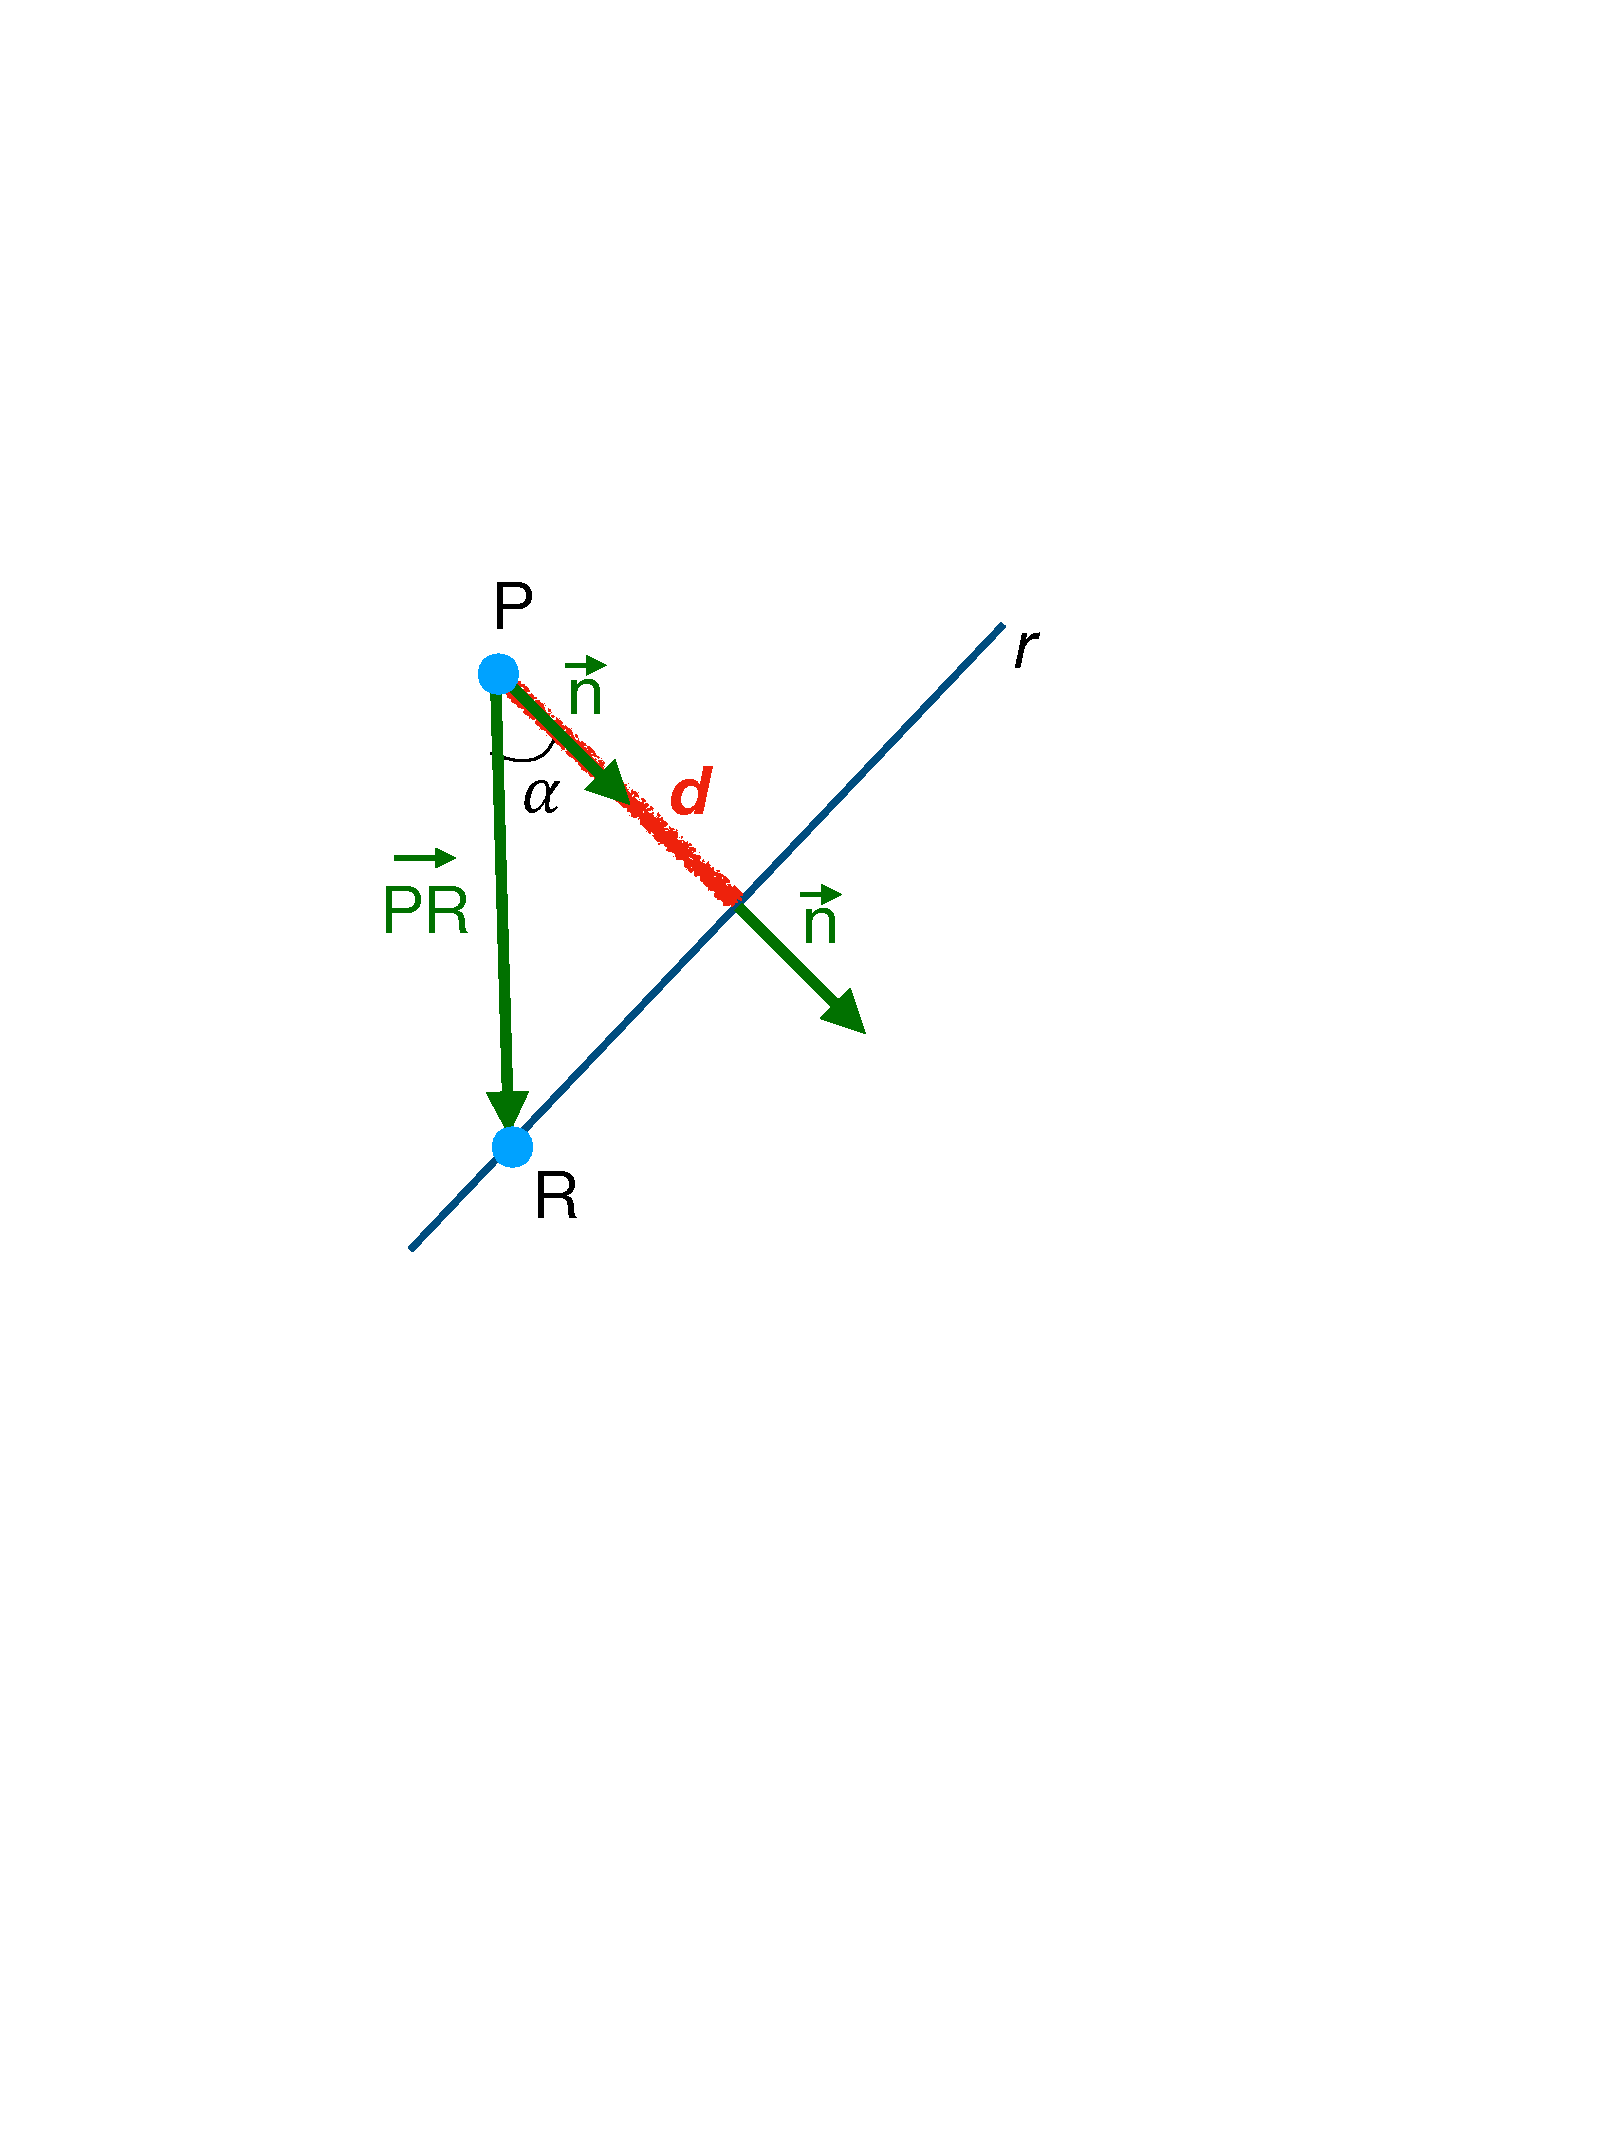
\includegraphics[width=0.4\textwidth]{img-sol/dem-dist-pr}
	\end{center}

	{
	\large
	
	Suposem que la recta $r$ vengui donada en forma general $Ax+By+C=0$. Recordem que el vector normal a la recta és $\vec n = (A,B)$.
	
	Si $R$ és un punt qualsevol de la recta i $\vec n$ és el seu vector normal, observam de l'esquema de la figura que la distància s'obté per trigonometria
	\[
		d = |\overrightarrow{PR}| \cos \alpha
	\]
	
	Per definició de producte escalar:
	\[
		\overrightarrow{PR} \cdot \vec n = |\overrightarrow{PR}|\, |\vec n| \, \cos \alpha
	\]
	
	Si aïllam $\cos \alpha$ i ho reemplaçam en la fórmula anterior, trobam:
	\[
		d = \dfrac{	\overrightarrow{PR} \cdot \vec n}{ |\vec n| } = \dfrac{
		(R_x-P_x, R_y-P_y)\cdot (A,B)}{\sqrt{A^2+B^2}}
	\]
	
	Si desenvolupam $(R_x-P_x, R_y-P_y)\cdot (A,B) = AR_x+B R_y - (AP_x+B P_y)=-C-(A P_x+B P_y)$. Aquí hem utilitzat el fet que el punt $R$ pertany a la recta i, per tant, compleix la seva equació $A R_x+B R_y+C=0$.
	
	Finalment
	
		\[d =  \dfrac{|A P_x+ B P_y +C|}{\sqrt{A^2+B^2}} \]
	
	el valor absolut $|\;|$ és per assegurar que les distàncies surtin positives.
	}
}

%%% Llocs o circumferencia
\newcommand{\pagecxxxi}{

\heading{Mètode de completar quadrats}

Quan tenim una identitat notable és evident que 

\[ x^2 - 2x + 1 = (x-1)^2 \]

Però, que passaria si només tinguessim $x^2-2x$?

\[ x^2 - 2x = \underbrace{ x^2 - 2x \mathbf{ + 1} } \mathbf{- 1 } = (x-1)^2 - 1\]

Com veim acabam de completar el quadrat de l'expressió.

\vso

\heading{Aplicació a la circumferència}

Ens donen l'equació general de la circumferència $x^2+y^2-4x+6y=3$ i en volem saber el centre i el radi. Per això, és convenient passar l'equació a forma canònica. Com ho feim? Completam quadrats!

Primer ajuntam les $x$ i els termes amb $y$

\[ \underbrace{x^2-4x}+\underbrace{y^2+6y}=3 \]

Completam quadrats de cada part

\[
	  \underbrace{x^2-4x+4}-4+\underbrace{y^2+6y+9}-9=3
\]

\[
	(x-2)^2 -4+(y+3)^2-9=3
\]

\[
	(x-2)^2 + (y+3)^2 = 16
\]

D'aquí fàcilment identificam el centre $O=(2,-3)$ i el radi $R=\sqrt{16}=4$.



}

%%% Demostracio ellipse
\newcommand{\pagecxxxii}{
	\heading{Exemple construcció el·lipse}
	\vspace{0.5cm}
	
	\begin{minipage}{0.5\textwidth}

\textbf{DADES}: Volem trobar l'equació de l'el·lipse que té focus a $F(4,0)$ i $F'(-4,0)$ i té semieix major $a=5$. 
\vso

El semieix menor es troba de $b=\sqrt{5^2-4^2}=3$.

Per a qualsevol punt $P(x,y)$ sobre l'el·lipse, es compleix que 
\[
d(P,F) + d(P,F')=2a=10
\]
			
\end{minipage}
\hspace{0.5cm}
\begin{minipage}{0.43\textwidth}
	
	\begin{center}	
		
		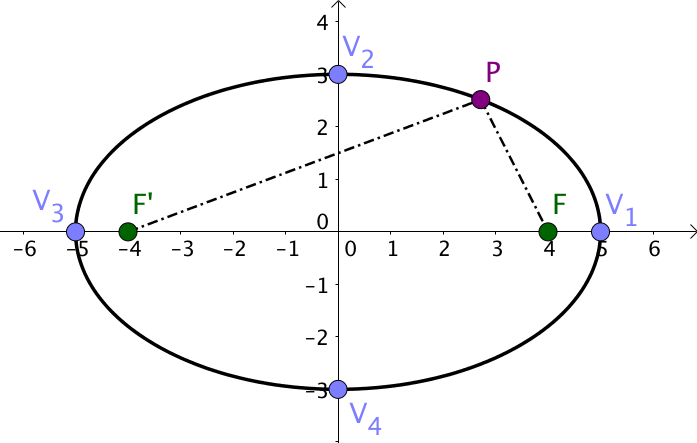
\includegraphics[width=0.9\textwidth]{img-sol/construccio-ellipse}
		
		\ggblink{https://www.geogebra.org/m/yEZzBKCS}
		
		
	\end{center}
\end{minipage}		

	Expressam les distàncies en components
	\[
		\sqrt{(x-4)^2+y^2} + \sqrt{(x+4)^2+y^2}=10
	\]	
	Aïllam la primera arrel i elevam al quadrat els dos membres
	\[
		(x-4)^2+y^2 = 100 +(x+4)^2+y^2 - 20\sqrt{(x+4)^2+y^2}
	\]	
	Tornam a aïllar l'arrel i elevam al quadrat un altre pic
	\[
		-16 x - 100  = - 20\sqrt{(x+4)^2+y^2}
	\]
	\[
		256 x^2 +3200 x + 10000  = 400 \left( (x+4)^2+y^2 \right)
	\]
	Simplificant els quadrats d'aquesta expressió trobam $144x^2+400y^2=3600$, que si dividim tot entre 3600 arribam a
	\[
		\dfrac{x^2}{25}+\dfrac{y^2}{9}=1
	\]
	
	
	
	
	
}


%%% Demostracio hiperbola
\newcommand{\pagecxxxiii}{
	\heading{Exemple construcció hipèrbola}
 \vspace{0.5cm}

	\begin{minipage}{0.5\textwidth}
	
	\textbf{DADES}: Volem trobar l'equació de la hipèrbola que té focus a $F(5,0)$ i $F'(-5,0)$ i té semieix major $a=4$. 
	\vso
	
	El semieix menor es troba de $b=\sqrt{5^2-4^2}=3$.
	
	Per a qualsevol punt $P(x,y)$ sobre la hipèrbola, es compleix que 
	\[
	d(P,F) - d(P,F')=\pm 2a= \pm 8
	\]
	
\end{minipage}
\hspace{0.5cm}
\begin{minipage}{0.43\textwidth}
	
	\begin{center}	
		
		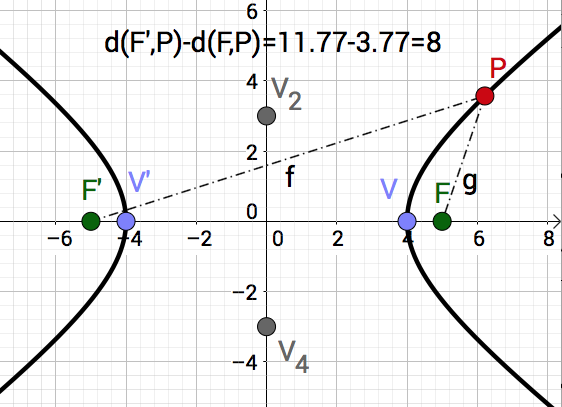
\includegraphics[width=0.9\textwidth]{img-sol/construccio-hiperbola}
		
		\ggblink{https://www.geogebra.org/m/CdRCjv8S}	
		
		
	\end{center}
\end{minipage}		

Expressam les distàncies en components
\[
\sqrt{(x-5)^2+y^2} - \sqrt{(x+5)^2+y^2}=\pm 8
\]	
Aïllam la primera arrel i elevam al quadrat els dos membres
\[
(x-5)^2+y^2 = 64 +(x+5)^2+y^2 + 16\sqrt{(x+5)^2+y^2}
\]	
Tornam a aïllar l'arrel i elevam al quadrat un altre pic
\[
-20 x - 64  =  16\sqrt{(x+5)^2+y^2}
\]
\[
400 x^2 +2560x + 4096  = 256 \left( (x+5)^2+y^2 \right)
\]
Simplificant els quadrats d'aquesta expressió trobam $144x^2-256y^2=2304$, que si dividim tot entre 2304 arribam a
\[
\dfrac{x^2}{16}-\dfrac{y^2}{9}=1
\]

}


%%% Demostracio parabola en general
\newcommand{\pagecxxxiv}{
	\heading{Exemple construcció paràbola obliqua}
 \vspace{0.5cm}

\begin{minipage}{0.5\textwidth}
	
	\textbf{DADES}: Volem trobar l'equació de la paràbola que té focus a $F(2,1)$ i recta directriu $r:\; y=x-5$. 
	\vso
	
	Per a qualsevol punt $A(x,y)$ sobre la paràbola, es compleix que 
	\[
	d(A,F)= d(A,r)
	\]
	
\end{minipage}
\hspace{0.5cm}
\begin{minipage}{0.43\textwidth}
	
	\begin{center}	
		
			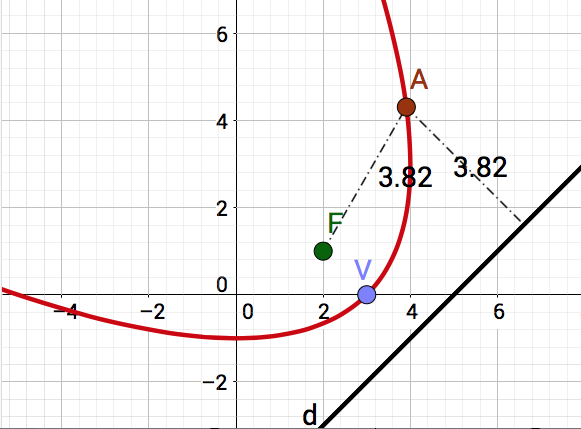
\includegraphics[width=0.9\textwidth]{img-sol/construccio-parabola}
		
			\ggblink{https://www.geogebra.org/m/b6JmdezZ}
		
		
	\end{center}
\end{minipage}	

Expressam les distàncies en components
\[
\sqrt{(x-2)^2+(y-1)^2} = \dfrac{|x-y-5|}{\sqrt{2}}
\]
Elevam al quadrat
\[
(x-2)^2+(y-1)^2 = \dfrac{(x-y-5)^2}{2}
\]
Multiplicam per tot i desenvolupam els quadrats:
\[
	2\left[ x^2-2x+4 +y^2-2y+1 \right] = x^2+y^2 -2xy -10x+10y+25
\]
Simplificant, arribam a l'equació de la paràbola obliqua:
\[
	x^2+y^2+2xy+2x-14y-15=0
\] 
}



%%% estadistica 1d
\newcommand{\pagecxlii}{
	
	\heading{Distribucions marginals}
	
	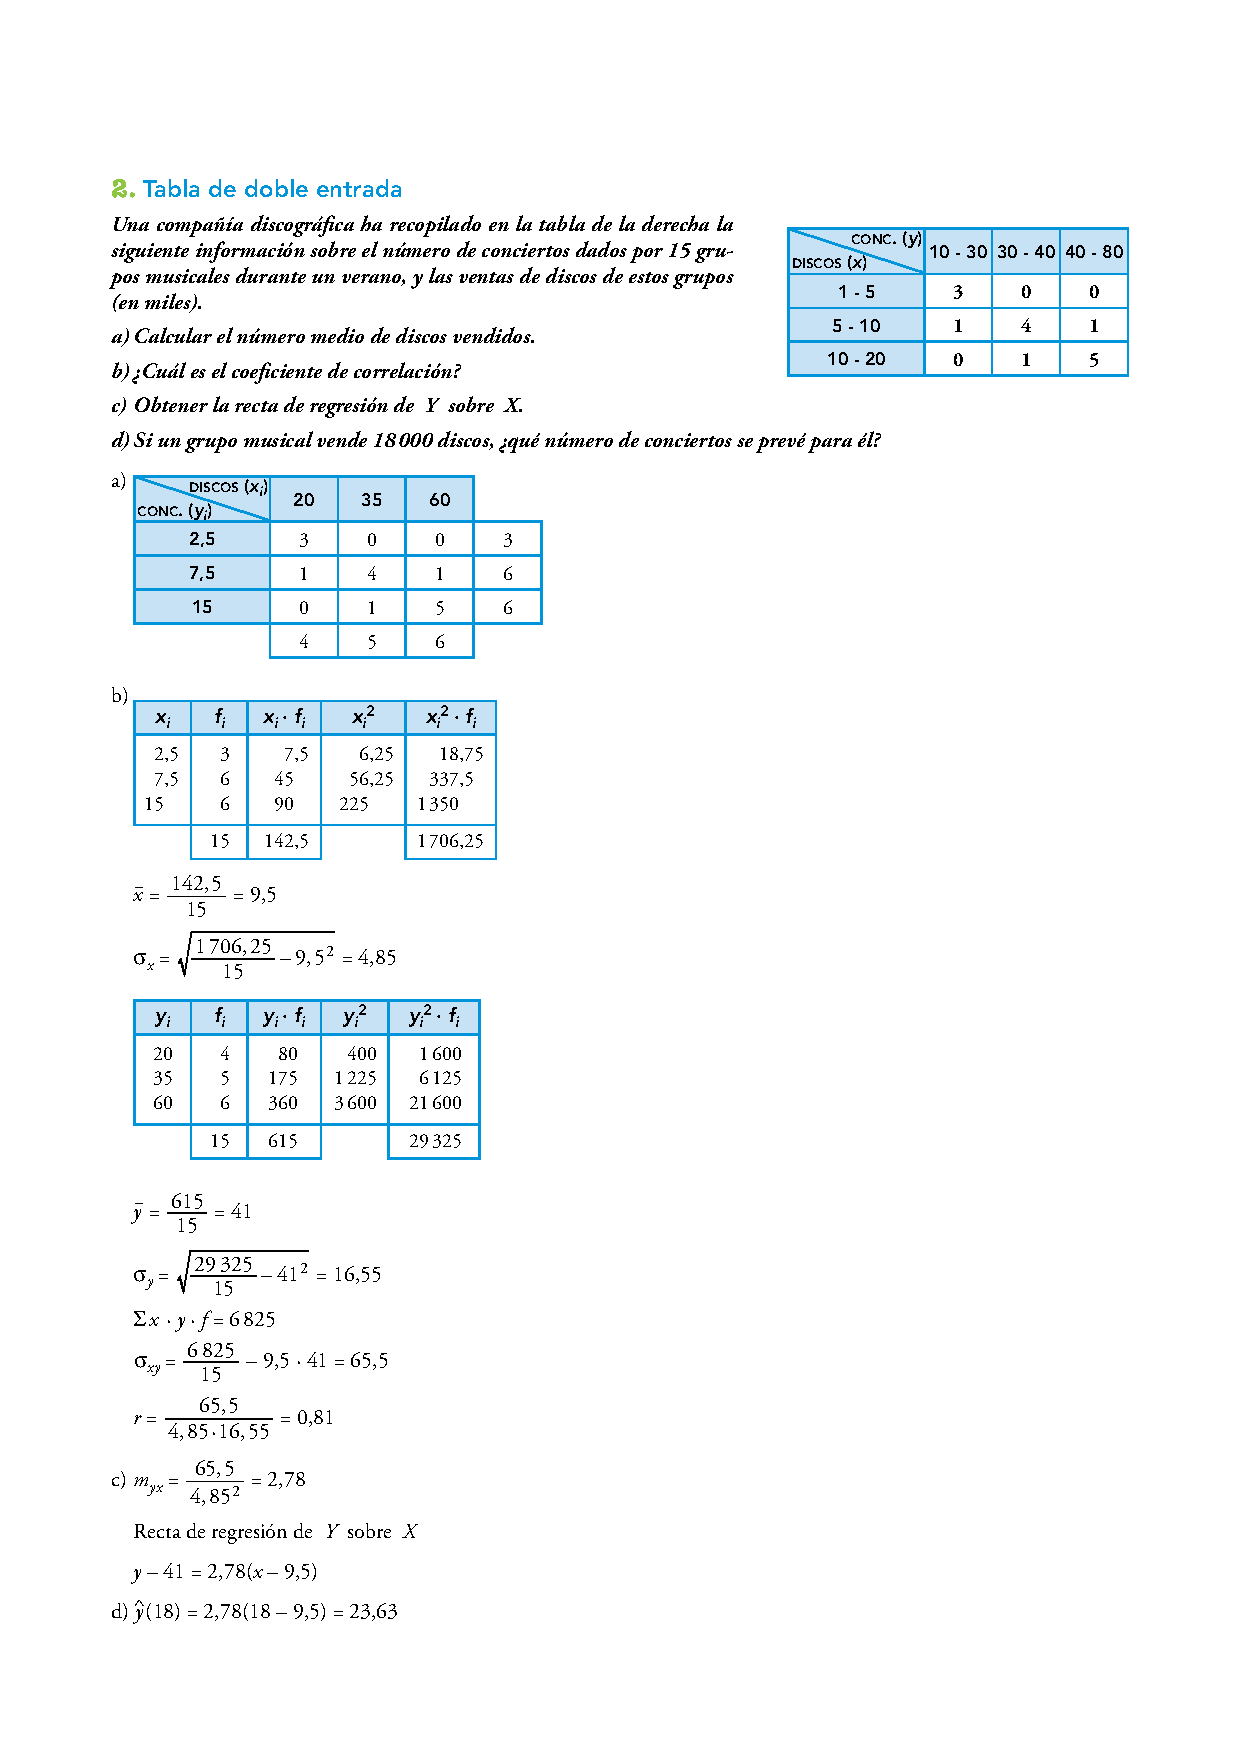
\includegraphics[width=\textwidth]{img-sol/p147-extra}
}


%%% estadistica nuvols i bimbolles
\newcommand{\pagecxlv}{
	
	\heading{Núvols de punts}
	
	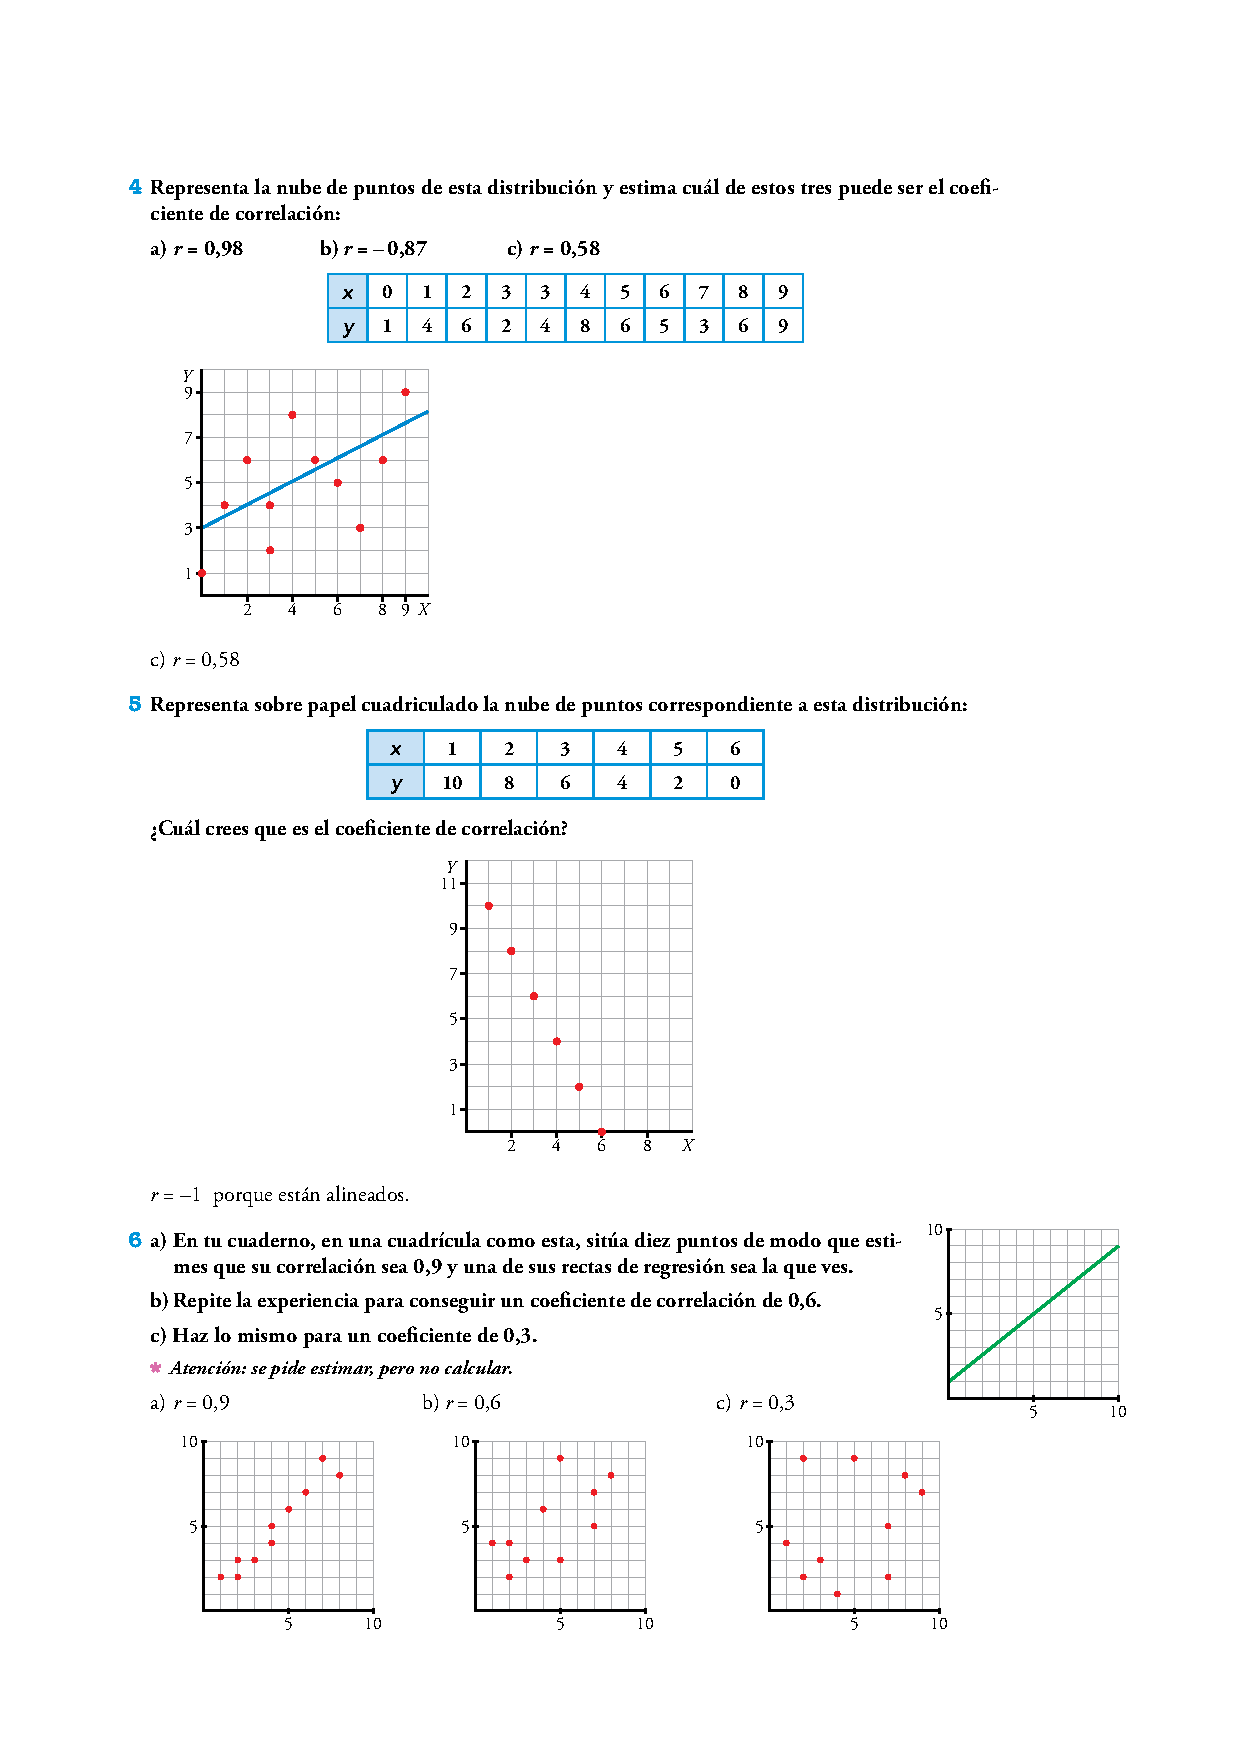
\includegraphics[width=\textwidth]{img-sol/p145-extra}
}


%%% estadistica: coeficent amb dades agrupades
\newcommand{\pagecxlvii}{
	
	\heading{Càlcul de $r$ amb dades agrupades}
	
	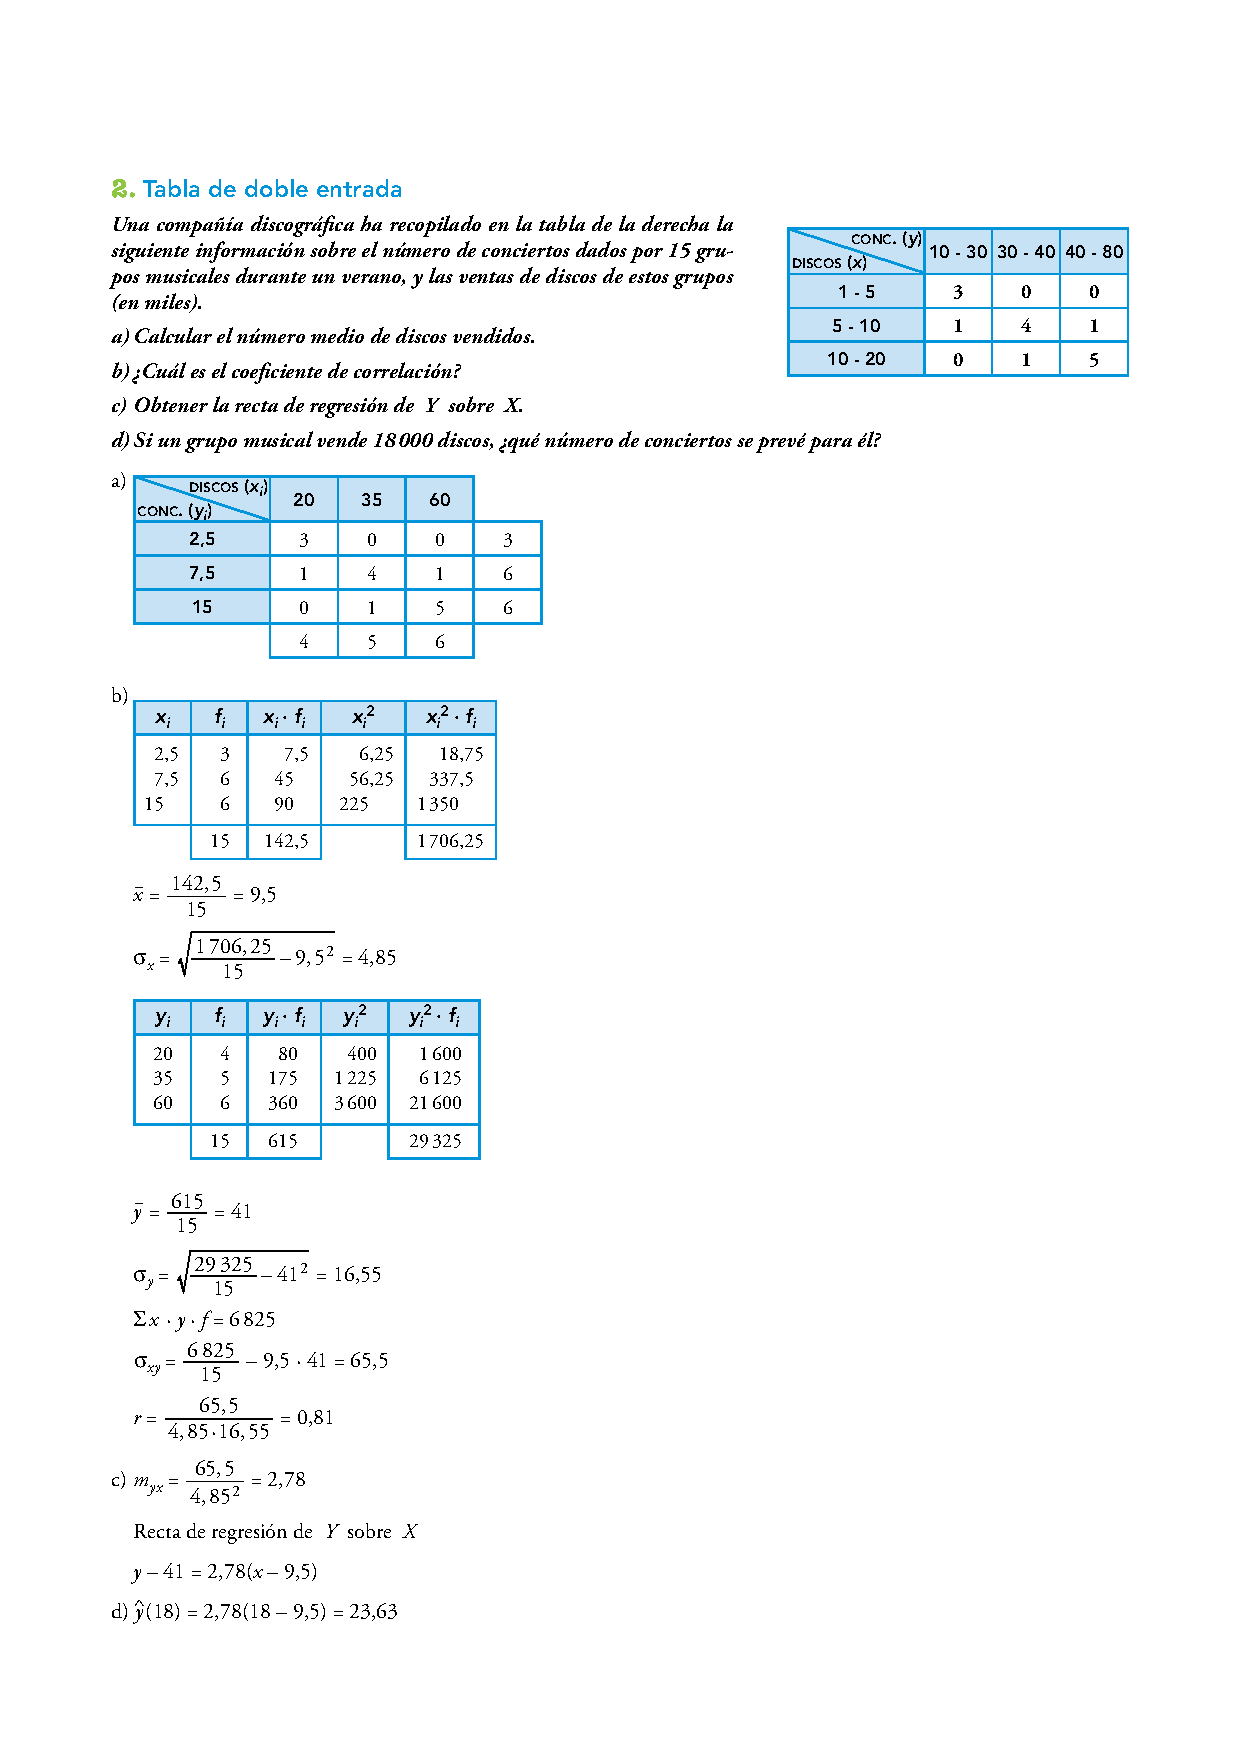
\includegraphics[width=\textwidth]{img-sol/p147-extra}
}


\newcommand{\pagecxlviii}{
	
	\heading{Recta X sobre Y}
	
	Si volem fer una predicció conegut el valor de $y$  trobar el valor de $x$, podem utilitzar l'equació de la recta de regressió $y=\bar y + \dfrac{\sigma_{xy}}{\sigma_x^2} (x-\bar x)$ i aïllar el valor de $x$.
	
	El més lògic, però és utilitzar la recta de regressió X sobre Y
	\[ x=\bar x + \dfrac{\sigma_{xy}}{\sigma_y^2} (y-\bar y) \]
	que ja ens proporcionarà directament el valor de $x$ conegut $y$.
	
	Cal assenyalar que quan $|r|\rightarrow 1$, les dues prediccions seran pràcticament iguals. Per correlacions febles, obtindrem valors molt distints, cosa que indica que la predicció és poc fiable.
}


\newcommand{\displaynotes}{
\vspace*{\fill}
\heading{Notes:}

\begin{flushright}
\begin{minipage}{0.74\paperwidth}
	\dotfill \par \vspace{0.25cm}
	\dotfill \par \vspace{0.25cm}
\dotfill \par \vspace{0.25cm}
\end{minipage}
\end{flushright}
\newpage
}
\newenvironment{pagesol}[2][]{
	\vspace*{-1.5cm}
	\begin{center}
		\ifodd#2
			\includegraphics[page=#2, scale=0.8, trim={1cm 2cm 1cm 1.8cm}, clip, frame]{./output-student/llibre-1bat-student.pdf}
		\else
			\includegraphics[page=#2, scale=0.8, trim={1cm 2cm 1cm 1.8cm}, clip, frame]{./output-student/llibre-1bat-student.pdf}
		\fi
	\end{center}
		\begin{minipage}{0.75\paperwidth}
			\begin{multicols}{2}
		}{
		\end{multicols}
		\end{minipage}
}

\newenvironment{pageandsol}[2][]{
\def\nonotes{#1}
\includepdf[pages=#2]{./output-student/llibre-1bat-student.pdf}
\newpage

\heading{Solucions de la pàgina #2:}
\normalfont
	\vspace{0.25cm}
}{
\vspace{0.25cm}

}

\newenvironment{pageandsolTwo}[2][]{
\includepdf[pages=#2]{./output-student/llibre-1bat-student.pdf}
\newpage

\heading{Solucions de la pàgina #2:}
\normalfont
	\vspace{0.25cm}
  \begin{multicols}{2}
}{
\end{multicols} 
 \vspace{0.25cm}

}

\setlength{\columnseprule}{0.4pt}
\begin{document}
	\thispagestyle{empty}
	\pagestyle{empty}

	\includepdf[pages=1]{./output-student/llibre-1bat-student.pdf}

	\includepdf[pages=2]{./output-student/llibre-1bat-student.pdf}

	\includepdf[pages=3]{./output-student/llibre-1bat-student.pdf}

	\includepdf[pages=4]{./output-student/llibre-1bat-student.pdf}

	\includepdf[pages=5]{./output-student/llibre-1bat-student.pdf}

	\includepdf[pages=6]{./output-student/llibre-1bat-student.pdf}

	\includepdf[pages=7]{./output-student/llibre-1bat-student.pdf}

	\includepdf[pages=8]{./output-student/llibre-1bat-student.pdf}

	\includepdf[pages=9]{./output-student/llibre-1bat-student.pdf}

\clearemptydoublepage\normalsize
  \begin{pageandsol}{10}
  \begin{enumerate}
\item[\fontfamily{phv}\selectfont\large\color{blue}\textbf{1. }] 

 \begin{tasks}[label-format=\bfseries\large](3)
	 \task $0.\hat 6$
	 \task $0.75$
	 \task $0.2\hat 3$
	 \task $0.24$
	 \task $0.875$
	 \task $0.\widehat {81}$
\end{tasks}

\mbox{}\vspace{0.25cm}
\item[\fontfamily{phv}\selectfont\large\color{blue}\textbf{2. }] 

 \begin{tasks}[label-format=\bfseries\large](3)
	 \task $233/99$
	 \task $431821/3300$
	 \task $1$
\end{tasks}

\mbox{}\vspace{0.25cm}
 \end{enumerate}

  \end{pageandsol}

\vspace{0.25cm} \hrule \vspace{0.25cm}
\pagex

\displaynotes


\clearemptydoublepage\normalsize
  \begin{pageandsol}{11}
  \begin{enumerate}
\item[\fontfamily{phv}\selectfont\large\color{blue}\textbf{5. }] 

 \begin{tasks}[label-format=\bfseries\large](3)
	 \task 5
	 \task 5
	 \task $\sqrt {10}-\pi $
\end{tasks}

\mbox{}\vspace{0.25cm}
\item[\fontfamily{phv}\selectfont\large\color{blue}\textbf{6. }] 

 \begin{tasks}[label-format=\bfseries\large](2)
	 \task 4
	 \task 2.2
	 \task 2
	 \task 9
\end{tasks}

\mbox{}\vspace{0.25cm}
\item[\fontfamily{phv}\selectfont\large\color{blue}\textbf{7. }] 

 \begin{tasks}[label-format=\bfseries\large](2)
	 \task $1\leq x<7$
	 \task $-3<x<5$
	 \task $2<x\leq 8$
	 \task $x<6$
\end{tasks}

\mbox{}\vspace{0.25cm}
\item[\fontfamily{phv}\selectfont\large\color{blue}\textbf{8. }] 

 \begin{tasks}[label-format=\bfseries\large](2)
	 \task $(2,5)$
	 \task $(4,+\infty )$
	 \task $[3,6)$
	 \task $(-\infty ,7]$
\end{tasks}

\mbox{}\vspace{0.25cm}
\item[\fontfamily{phv}\selectfont\large\color{blue}\textbf{9. }] 

 \begin{tasks}[label-format=\bfseries\large](3)
	 \task $(26,100]$
	 \task $[0,18]$
	 \task $(2,+\infty )$
	 \task $[100,1000)$
	 \task $(-\infty ,25)$
	 \task $[0,+\infty )$
	 \task $(1,9)$
\end{tasks}

\mbox{}\vspace{0.25cm}
 \end{enumerate}

  \end{pageandsol}


\displaynotes


\clearemptydoublepage\normalsize
  \begin{pageandsol}{12}
  \begin{enumerate}
\item[\fontfamily{phv}\selectfont\large\color{blue}\textbf{10. }] 

 \begin{tasks}[label-format=\bfseries\large](3)
	 \task $(-4,6)$
	 \task $(-14/3,2/3)$
	 \task $(-10.001,-9.999)$
\end{tasks}

\mbox{}\vspace{0.25cm}
\item[\fontfamily{phv}\selectfont\large\color{blue}\textbf{11. }] 

 \begin{tasks}[label-format=\bfseries\large](3)
	 \task $(5.5,1.5)$
	 \task $(-5.5,1.5)$
	 \task $(-0.5,2.5)$
\end{tasks}

\mbox{}\vspace{0.25cm}
\item[\fontfamily{phv}\selectfont\large\color{blue}\textbf{12. }] 

 \begin{tasks}[label-format=\bfseries\large](3)
	 \task $x=$ 5 \, i \, --5
	 \task $x=$ 4
	 \task $x=$ --10 \, i \, 4
\end{tasks}

\mbox{}\vspace{0.25cm}
\item[\fontfamily{phv}\selectfont\large\color{blue}\textbf{13. }] 

 \begin{tasks}[label-format=\bfseries\large](1)
	 \task $(-1,1)$
	 \task $(-\infty ,-1]\cup [1,+\infty ]$
	 \task $(-\infty ,2)\cup (4,+\infty )$
	 \task $(-\infty ,2]\cup [4,+\infty )$
\end{tasks}

\mbox{}\vspace{0.25cm}
\item[\fontfamily{phv}\selectfont\large\color{blue}\textbf{14. }] 

$-3$ \, i \, $9$. $-5.5$ \, i \, $1.5$. $9-(-5.5)=14.5$
\mbox{}\vspace{0.25cm}

\item[\fontfamily{phv}\selectfont\large\color{blue}\textbf{15. }] 

$[-3, 8)$
\mbox{}\vspace{0.25cm}

\item[\fontfamily{phv}\selectfont\large\color{blue}\textbf{16. }] 

$[5,11]$
\mbox{}\vspace{0.25cm}

\item[\fontfamily{phv}\selectfont\large\color{blue}\textbf{17. }] 

 \begin{tasks}[label-format=\bfseries\large](2)
	 \task $A\cap B=\emptyset $;\par $A\cup B=[-11,-9] \cup (-1,6)$;\par $A-B=A$
	 \task $A\cap B=B$;\, $A\cup B=A$;\par $A-B=[-5,3]\cup [4,5]$
\end{tasks}

\mbox{}\vspace{0.25cm}
\item[\fontfamily{phv}\selectfont\large\color{blue}\textbf{18. }] 

 \begin{tasks}[label-format=\bfseries\large](3)
	 \task $\sqrt [{6}]{5} $
	 \task $\sqrt [{8}]{8} $
	 \task $\sqrt [{8}]{x^{7} } $
\end{tasks}

\mbox{}\vspace{0.25cm}
\item[\fontfamily{phv}\selectfont\large\color{blue}\textbf{19. }] 

 \begin{tasks}[label-format=\bfseries\large](3)
	 \task $2\,\sqrt [{}]{2} $
	 \task $9\,\sqrt [{}]{3} $
	 \task $\sqrt [{3}]{6} $
	 \task $2\,\sqrt [{4}]{2} $
	 \task $\sqrt [{3}]{3} $
	 \task $\sqrt [{3}]{49} $
	 \task $\sqrt [{8}]{7} $
	 \task $\sqrt {2} $
\end{tasks}

\mbox{}\vspace{0.25cm}
\item[\fontfamily{phv}\selectfont\large\color{blue}\textbf{20. }] 

 \begin{tasks}[label-format=\bfseries\large](2)
	 \task $\sqrt [{4}]{2^{3} } =\sqrt [{12}]{2^{9} } $
	 \task $\sqrt {7} =\sqrt [{16}]{7^{8} } $
	 \task $\sqrt [{4}]{a^{6} } =\sqrt {a^{3} } $
	 \task $\sqrt [{6}]{5^{12} } =\sqrt [{3}]{5^{6} } =5^{2} $
\end{tasks}

\mbox{}\vspace{0.25cm}
 \end{enumerate}

  \end{pageandsol}


\displaynotes


\clearemptydoublepage\normalsize
  \begin{pageandsol}{13}
  \begin{enumerate}
\item[\fontfamily{phv}\selectfont\large\color{blue}\textbf{21. }] 

 \begin{tasks}[label-format=\bfseries\large](2)
	 \task $\sqrt [{3}]{5/4} $
	 \task $\sqrt [{12}]{2^{3} \cdot 3} $
	 \task $\sqrt [{12}]{5^{7} } $
	 \task $2^{3} $
	 \task $2^{4} \cdot \sqrt [{5}]{2^{4} } $
	 \task $\sqrt [{}]{5} $
	 \task 3
	 \task $5^{2} $
\end{tasks}

\mbox{}\vspace{0.25cm}
\item[\fontfamily{phv}\selectfont\large\color{blue}\textbf{22. }] 

 \begin{tasks}[label-format=\bfseries\large](3)
	 \task  $15\,\sqrt [{}]{11} $
	 \task $6\,\sqrt [{3}]{2} $
	 \task $-\sqrt [{}]{6} /5$
	 \task $-14\,\sqrt [{4}]{2} /3$
	 \task $41\,\sqrt [{}]{3} /15$
	 \task $13\,\sqrt [{}]{2} /5$
\end{tasks}

\mbox{}\vspace{0.25cm}
\item[\fontfamily{phv}\selectfont\large\color{blue}\textbf{23. }] 

$(2+a)^{2} +4(2+a)\sqrt {a} +4a$
\mbox{}\vspace{0.25cm}

\item[\fontfamily{phv}\selectfont\large\color{blue}\textbf{24. }] 

 \begin{tasks}[label-format=\bfseries\large](2)
	 \task $\frac {\sqrt [{3}]{3^{2} } }{3} $
	 \task $\frac {3}{4} \,\sqrt [{4}]{2^{3} }$
	 \task $3(\sqrt {2+1} )$
	 \task $3+2\sqrt {2} $
	 \task $(\sqrt {10} -\sqrt {6} )/2$
	 \task $-(9+4\sqrt {5} )$
\end{tasks}

\mbox{}\vspace{0.25cm}
\item[\fontfamily{phv}\selectfont\large\color{blue}\textbf{25. }] 

 \begin{tasks}[label-format=\bfseries\large](2)
	 \task $3\sqrt {6}$
	 \task $\frac {\sqrt [{4}]{2^{3} } }{2} $
	 \task $\frac {\sqrt {3} }{2} $
	 \task 35
	 \task $2^{-64/15} $
	 \task $33/4-5\sqrt {2} $
\end{tasks}

\mbox{}\vspace{0.25cm}
 \end{enumerate}

  \end{pageandsol}


\displaynotes


\clearemptydoublepage\normalsize
  \begin{pageandsol}{14}
  \begin{enumerate}
\item[$\bullet$] {\fontfamily{phv}\selectfont\large\color{blue}\textbf{Autoavaluació: }} 


\mbox{}\vspace{0.25cm}

\item[\fontfamily{phv}\selectfont\large\color{blue}\textbf{1. }] 

$x=-10$ \, i \, $x=4$
\mbox{}\vspace{0.25cm}

\item[\fontfamily{phv}\selectfont\large\color{blue}\textbf{2. }] 

$\sqrt [8]{x^3}$
\mbox{}\vspace{0.25cm}

\item[\fontfamily{phv}\selectfont\large\color{blue}\textbf{3. }] 

$13+4\sqrt {3}$
\mbox{}\vspace{0.25cm}

\item[\fontfamily{phv}\selectfont\large\color{blue}\textbf{4. }] 

$\dfrac {4\sqrt {5}}{5}$
\mbox{}\vspace{0.25cm}

\item[\fontfamily{phv}\selectfont\large\color{blue}\textbf{5. }] 

$\frac {13}{3}\sqrt [3]{2}$
\mbox{}\vspace{0.25cm}

\item[\fontfamily{phv}\selectfont\large\color{blue}\textbf{6. }] 

$\dfrac {16-5\sqrt {15}}{-7}$
\mbox{}\vspace{0.25cm}

\item[\fontfamily{phv}\selectfont\large\color{blue}\textbf{7. }] 

$(-1,\,6]$
\mbox{}\vspace{0.25cm}

 \end{enumerate}

  \end{pageandsol}


\displaynotes


	\includepdf[pages=15]{./output-student/llibre-1bat-student.pdf}
\newpage
\pagexv
\newpage

\clearemptydoublepage\normalsize
  \begin{pageandsol}{16}
  \begin{enumerate}
\item[\fontfamily{phv}\selectfont\large\color{blue}\textbf{1. }] 

 \begin{tasks}[label-format=\bfseries\large](1)
	 \task $4x^2-20xy+25y^2$
	 \task $9x^2 +2xy+y^2/9$
	 \task $625-250+25/x^2$
	 \task $9a^2-6ab+b^2$
	 \task $a^4+2a^2b^2+b^4$
	 \task $9y^2/25 - 12/5+4/y^2$
\end{tasks}

\mbox{}\vspace{0.25cm}
\item[\fontfamily{phv}\selectfont\large\color{blue}\textbf{2. }] 

 \begin{tasks}[label-format=\bfseries\large](2)
	 \task $(a^2+3)^2$
	 \task $(3x-1)^2$
	 \task $(b-5)^2$
	 \task $(2y+3)^2$
	 \task $(a^2-1)^2$
	 \task $(y^2+3)^2$
\end{tasks}

\mbox{}\vspace{0.25cm}
\item[\fontfamily{phv}\selectfont\large\color{blue}\textbf{3. }] 

 \begin{tasks}[label-format=\bfseries\large](3)
	 \task $16x^4-9y^2$
	 \task $4x^4-64$
	 \task $-x^4+9x^2$
\end{tasks}

\mbox{}\vspace{0.25cm}
 \end{enumerate}

  \end{pageandsol}

\vspace{0.25cm} \hrule \vspace{0.25cm}
\pagexvi

\newpage


\clearemptydoublepage\normalsize
  \begin{pageandsol}{17}
  \begin{enumerate}
\item[\fontfamily{phv}\selectfont\large\color{blue}\textbf{4. }] 

 \begin{tasks}[label-format=\bfseries\large](1)
	 \task  $Q(x)=3x^{3}+4x^{2}-x+2$;\, $R(x)=-4$
	 \task $Q(x)=2x+2$;\, $R(x)=2x-1$
	 \task $Q(x)=a(x^{3}+ x^{2}+ x+ 1)$;\, $R(x)=a+b$
	 \task $Q(x)=x^{8}+ x^{6}+ x^{4}+ x^{2}+ 1$;\, $R(x)=0$ 
\end{tasks}

\mbox{}\vspace{0.25cm}
\item[\fontfamily{phv}\selectfont\large\color{blue}\textbf{5. }] 

 \begin{tasks}[label-format=\bfseries\large](1)
	 \task $Q=2x^2-4x-1$;\, $R=17x+11$
	 \task $Q=-2$;\, $R=-4x^2+x+10$
	 \task $Q=-2x^2+2$;\, $R=12x^2-5x-13$
	 \task $Q=-2x^2+3$;\, $R=-3x^2+8$
	 \task $Q=-6x^2$;\, $R=7x^2+1$ 
\end{tasks}

\mbox{}\vspace{0.25cm}
\item[\fontfamily{phv}\selectfont\large\color{blue}\textbf{6. }] 

 \begin{tasks}[label-format=\bfseries\large](1)
	 \task $Q=-3x-1$;\, $R=-1$
	 \task $Q=x^3+4x^2+8x+14$;\, $R=29$
	 \task $Q=4x^2-7x+7$;\, $R=-8$
	 \task $Q=x^2+3x$;\, $R=1$ 
\end{tasks}

\mbox{}\vspace{0.25cm}
 \end{enumerate}

  \end{pageandsol}


\displaynotes


\clearemptydoublepage\normalsize
  \begin{pageandsol}{18}
  \begin{enumerate}
\item[\fontfamily{phv}\selectfont\large\color{blue}\textbf{7. }] 

 \begin{tasks}[label-format=\bfseries\large](3)
	 \task $R=458$
	 \task $R=32$
	 \task $R=0$
\end{tasks}

\mbox{}\vspace{0.25cm}
\item[\fontfamily{phv}\selectfont\large\color{blue}\textbf{8. }] 

Per exemple $q(x)=p-r=x^6-4x^4-4x^2+x+1$ que donaria quocient 1.
\mbox{}\vspace{0.25cm}

\item[\fontfamily{phv}\selectfont\large\color{blue}\textbf{9. }] 

$D=d\cdot q + r$. Per exemple, si ens inventam $d=2x+1$, obtenim $D=2x^3-4x^2-7x-4$
\mbox{}\vspace{0.25cm}

\item[\fontfamily{phv}\selectfont\large\color{blue}\textbf{10. }] 

 \begin{tasks}[label-format=\bfseries\large](1)
	 \task $(x-3)^2$
	 \task $(x^2+4)^2$
	 \task $(x+\sqrt {5}y)^2$
	 \task NO
	 \task NO
	 \task $(x+6)(x-6)$
	 \task NO
	 \task $(\sqrt {5}x+\sqrt {11})(\sqrt {5}x-\sqrt {11})$
	 \task $(x^2+\sqrt {3}y)(x^2-\sqrt {3}y)$
\end{tasks}

\mbox{}\vspace{0.25cm}
\item[\fontfamily{phv}\selectfont\large\color{blue}\textbf{11. }] 

 \begin{tasks}[label-format=\bfseries\large](1)
	 \task $x(x-8)$
	 \task $(4x+3)(x-1)$
	 \task $x(x+2)(x-2)$
	 \task $x(x^2+25)$
	 \task $3x(x+1)^2$
	 \task $(x+2)(x-2)(x^2+4)$
	 \task $(2x-1)^2$
	 \task $x^3(x-2)$
\end{tasks}

\mbox{}\vspace{0.25cm}
 \end{enumerate}

  \end{pageandsol}


\displaynotes


\clearemptydoublepage\normalsize
  \begin{pageandsol}{19}
  \begin{enumerate}
\item[\fontfamily{phv}\selectfont\large\color{blue}\textbf{12. }] 

 \begin{tasks}[label-format=\bfseries\large](1)
	 \task  $3(x+2)\cdot (x+1)$
	 \task $x^{3}\cdot (x+3)\cdot (x-3)$
	 \task $4(x+3)\cdot (x+1)\cdot (x-1)$
	 \task $-2(x+1)^{2}\cdot (x-3)$
	 \task $x\cdot (x^{3}-x^{2}+8x-4)$
	 \task ($x+1)^{2}\cdot (x-2)$
	 \task $2(x+1)\cdot (x-2)\cdot (x-5)$
	 \task $x^{2}\cdot (x+1)\cdot (x-3)$
	 \task $(x+4)\cdot (x+1)\cdot (x-2)$ 
\end{tasks}

\mbox{}\vspace{0.25cm}
\item[\fontfamily{phv}\selectfont\large\color{blue}\textbf{13. }] 

Per a qualsevol valor de $m$
\mbox{}\vspace{0.25cm}

\item[\fontfamily{phv}\selectfont\large\color{blue}\textbf{14. }] 

 \begin{tasks}[label-format=\bfseries\large](3)
	 \task $\dfrac {x}{(x+1)(x-2)}$
	 \task $\dfrac {x-1}{(x-2)(x+4)}$
	 \task Igual
\end{tasks}

\mbox{}\vspace{0.25cm}
 \end{enumerate}

  \end{pageandsol}


\displaynotes


\clearemptydoublepage\normalsize
  \begin{pageandsol}{20}
  \begin{enumerate}
\item[\fontfamily{phv}\selectfont\large\color{blue}\textbf{15. }] 

 \begin{tasks}[label-format=\bfseries\large](2)
	 \task $\dfrac {x(x+2)}{x^2+5}$
	 \task $\dfrac {a-5}{7a+4}$
	 \task $\dfrac {x+3y}{4}$
	 \task $\dfrac {2ab+3}{(a+1)(a-1)}$
\end{tasks}

\mbox{}\vspace{0.25cm}
\item[\fontfamily{phv}\selectfont\large\color{blue}\textbf{16. }] 

 \begin{tasks}[label-format=\bfseries\large](3)
	 \task $x(x+1)$
	 \task $x^2(x+1)(x-1)$
	 \task $(x-1)^2 (x-2)$
\end{tasks}

\mbox{}\vspace{0.25cm}
\item[\fontfamily{phv}\selectfont\large\color{blue}\textbf{17. }] 

 \begin{tasks}[label-format=\bfseries\large](1)
	 \task  $\dfrac {x-1}{3x(x+2)} $
	 \task $\dfrac {2(x+5)}{(x+1)^{2} } $
	 \task $\dfrac {x-1}{x(x+2)} $
	 \task \textit {No es pot}
	 \task $\dfrac {(x^{2} +x+1)(x-1)}{x^{} } $
	 \task $\dfrac {1}{x+2} $
	 \task $\dfrac {x+2}{x-1} $
	 \task $\dfrac {2(x^{4} -x^{3} +x^{2} -x+1)}{x} $
\end{tasks}

\mbox{}\vspace{0.25cm}
\item[\fontfamily{phv}\selectfont\large\color{blue}\textbf{18. }] 

 \begin{tasks}[label-format=\bfseries\large](2)
	 \task $\dfrac {-2x+6}{3x(x-4)}$
	 \task $\dfrac {-4x^2+3x-1}{(x-1)^2 (x+1)}$
\end{tasks}

\mbox{}\vspace{0.25cm}
 \end{enumerate}

  \end{pageandsol}


\displaynotes


\clearemptydoublepage\normalsize
  \begin{pageandsol}{21}
  \begin{enumerate}
\item[\fontfamily{phv}\selectfont\large\color{blue}\textbf{19. }] 

 \begin{tasks}[label-format=\bfseries\large](2)
	 \task $\dfrac {6x^2+2x+4}{x(x^2+1)}$
	 \task $\dfrac {4x-5}{(x-2)(x+1)}$
	 \task $\dfrac {-1}{(x+3)(x-1)}$
	 \task $\dfrac {x+3}{x^2+3}$
\end{tasks}

\mbox{}\vspace{0.25cm}
\item[\fontfamily{phv}\selectfont\large\color{blue}\textbf{20. }] 

 \begin{tasks}[label-format=\bfseries\large](2)
	 \task $-\dfrac {(4x^2+x+1)}{x^3}$
	 \task $-\dfrac {(7x+2)}{x(x+3)}$
\end{tasks}

\mbox{}\vspace{0.25cm}
\item[\fontfamily{phv}\selectfont\large\color{blue}\textbf{21. }] 

 \begin{tasks}[label-format=\bfseries\large](2)
	 \task  $\dfrac {-4x}{(x+1)(x-1)} $
	 \task $\dfrac {-2}{x+1} $
	 \task $\dfrac {-1}{x-1} $
	 \task $\dfrac {-2t+3}{t(t+2)} $
	 \task 0
	 \task $\dfrac {1-x^{2} }{x^{2} } $
	 \task $\dfrac {3x^{2} +5}{x(x+1)^{2} } $
\end{tasks}

\mbox{}\vspace{0.25cm}
\item[\fontfamily{phv}\selectfont\large\color{blue}\textbf{22. }] 

 \begin{tasks}[label-format=\bfseries\large](1)
	 \task $\dfrac {-(a+y)(x+y)(a+x-y)}{(a-y)(x-y)(a+x+y)}$
	 \task $\dfrac {(2x+3y)(2y-x)}{(3x+y)(5x+3y)}$
	 \task $\dfrac {(x-2)(x^2+x-1)}{x^2-3x-2}$
\end{tasks}

\mbox{}\vspace{0.25cm}
\item[\fontfamily{phv}\selectfont\large\color{blue}\textbf{23. }] 

a) $1, –1, 2, –2$;\, Arrel $x = 1$.\par b) $1, –1, 3, –3$;\, Arrels: $–3$ \, i \, $–1$. \par c) $1, –1, 3, –3, 9, –9$;\, Arrels: 2 \, i \, 1;\, \par d) $0, 1, –1, 2, –2, 3, –3, 6, –6$;\, Arrels 0 \, i \, $–2$.
\mbox{}\vspace{0.25cm}

 \end{enumerate}

  \end{pageandsol}


\displaynotes


\clearemptydoublepage\normalsize
  \begin{pageandsol}{22}
  \begin{enumerate}
\item[\fontfamily{phv}\selectfont\large\color{blue}\textbf{24. }] 

 \begin{tasks}[label-format=\bfseries\large](1)
	 \task $x=-\dfrac {75}{17}$ \, i \, $x=0$
	 \task $x=\frac {2\pm 2\sqrt {37}}{3}$
	 \task $x=\pm 1$
	 \task $x=\pm \sqrt {\dfrac {3\pm \sqrt {24}}{10}}$
\end{tasks}

\mbox{}\vspace{0.25cm}
\item[\fontfamily{phv}\selectfont\large\color{blue}\textbf{25. }] 

 \begin{tasks}[label-format=\bfseries\large](2)
	 \task  $x=1,\,2,\,-2$
	 \task $x=0,\,5,\,-5$
	 \task $x=1,\,-2$
	 \task $x=\pm 2,\,3,\,-1$
	 \task $x=1,\,3,\,5,\,-4$
	 \task $x=1$
	 \task $x=-2,\,-1,\,2$
	 \task $x=-3,\,-1,\,2$
	 \task $x=-2,\,2,\,4$
	 \task $x=-3,\,-2,\,1$
	 \task $x=-3,\,3,\,-2,\,2$
	 \task $x=-1,\,0,\,5$ 
\end{tasks}

\mbox{}\vspace{0.25cm}
\item[\fontfamily{phv}\selectfont\large\color{blue}\textbf{26. }] 

No pot tenir terme independent, és a dir, $a_0=0$.
\mbox{}\vspace{0.25cm}

\item[\fontfamily{phv}\selectfont\large\color{blue}\textbf{27. }] 

La suma de tots els coeficients ha d'ésser zero, és a dir, $a_n + a_{n-1}+\cdots +a_1+a_0=0$.
\mbox{}\vspace{0.25cm}

\item[\fontfamily{phv}\selectfont\large\color{blue}\textbf{28. }] 

El nombre és 12. $2x+7+3/2x=6x-23$
\mbox{}\vspace{0.25cm}

\item[\fontfamily{phv}\selectfont\large\color{blue}\textbf{29. }] 

Les dimensions són 30 m \, i \, 24 m. Planteig: $\dfrac {36}{54}=\dfrac {x}{36}$. 
\mbox{}\vspace{0.25cm}

\item[\fontfamily{phv}\selectfont\large\color{blue}\textbf{30. }] 

 \begin{tasks}[label-format=\bfseries\large](3)
	 \task $x=6$
	 \task $x=2$
	 \task $x=3$
\end{tasks}

\mbox{}\vspace{0.25cm}
 \end{enumerate}

  \end{pageandsol}


\displaynotes


\clearemptydoublepage\normalsize
  \begin{pageandsol}{23}
  \begin{enumerate}
\item[\fontfamily{phv}\selectfont\large\color{blue}\textbf{31. }] 

 \begin{tasks}[label-format=\bfseries\large](2)
	 \task  $x= \dfrac {2}{3},\,-\dfrac {1}{2}$
	 \task $x=2,\,\dfrac {1}{7}$
	 \task $x=2,\,-\dfrac {3}{5}$
	 \task $\dfrac {1\pm \sqrt {41}}{4}$
\end{tasks}

\mbox{}\vspace{0.25cm}
\item[\fontfamily{phv}\selectfont\large\color{blue}\textbf{32. }] 

 \begin{tasks}[label-format=\bfseries\large](3)
	 \task $x=-\dfrac {11}{17}$
	 \task $x=S.S.$
	 \task $x=S.S.$
\end{tasks}

\mbox{}\vspace{0.25cm}
\item[\fontfamily{phv}\selectfont\large\color{blue}\textbf{33. }] 

 \begin{tasks}[label-format=\bfseries\large](2)
	 \task  $x=4$
	 \task $x=4$
	 \task $x=9$
	 \task $x=7$
	 \task $x=2$
	 \task $x=38414$
	 \task $x=10$
	 \task $x=3$
	 \task $x=11$
	 \task $x=29$
	 \task $x=14$
	 \task $x=1$
\end{tasks}

\mbox{}\vspace{0.25cm}
 \end{enumerate}

  \end{pageandsol}


\displaynotes


\clearemptydoublepage\normalsize
  \begin{pageandsol}{24}
  \begin{enumerate}
\item[\fontfamily{phv}\selectfont\large\color{blue}\textbf{34. }] 

 \begin{tasks}[label-format=\bfseries\large](2)
	 \task  $x=1;\, y=16$
	 \task $x=6;\, y=8$
	 \task $x=10;\, y=2$
	 \task $x=4;\, y=7$
	 \task $x=3;\, y=1$
	 \task $x=-2;\, y=8$ 
\end{tasks}

\mbox{}\vspace{0.25cm}
\item[\fontfamily{phv}\selectfont\large\color{blue}\textbf{35. }] 

 \begin{tasks}[label-format=\bfseries\large](1)
	 \task  $x=-1;\, y=4$
	 \task $x=-\dfrac {3}{7};\, y=\dfrac {1}{7}$ \, i \, $x=0;\, y=1$
	 \task $x=-\dfrac {1}{2};\, y=-2$ \, i \, $x=\dfrac {1}{2};\, y=2$
	 \task $x=9;\, y=4$ 
\end{tasks}

\mbox{}\vspace{0.25cm}
\item[\fontfamily{phv}\selectfont\large\color{blue}\textbf{36. }] 

 \begin{tasks}[label-format=\bfseries\large](1)
	 \task  $x=7;\, y=2;\, z=11$
	 \task $x=4;\, y=-3;\, z=0$
	 \task $x=-1;\, y=4;\, z=4$
	 \task $x=8;\, y=4;\, z=-3$ 
\end{tasks}

\mbox{}\vspace{0.25cm}
\item[\fontfamily{phv}\selectfont\large\color{blue}\textbf{37. }] 

 \begin{tasks}[label-format=\bfseries\large](1)
	 \task  $x=1;\, y=-5;\, z=4$
	 \task $x=-1;\, y=-2;\, z=-2$
	 \task $x=15;\, y=2;\, z=1$
	 \task $x=3;\, y=4;\, z=9$ 
\end{tasks}

\mbox{}\vspace{0.25cm}
 \end{enumerate}

  \end{pageandsol}


\displaynotes


\clearemptydoublepage\normalsize
  \begin{pageandsol}{25}
  \begin{enumerate}
\item[\fontfamily{phv}\selectfont\large\color{blue}\textbf{38. }] 

 \begin{tasks}[label-format=\bfseries\large](1)
	 \task  $x=1;\, y=-2;\, z=3$
	 \task $x=4;\, y=2;\, z=-3$
	 \task $x=1;\, y=-1;\, z=0$
	 \task $x=2;\, y=\dfrac {1}{5};\, z=-1$ 
\end{tasks}

\mbox{}\vspace{0.25cm}
\item[\fontfamily{phv}\selectfont\large\color{blue}\textbf{39. }] 

 \begin{tasks}[label-format=\bfseries\large](1)
	 \task  $x=\dfrac {16}{15};\, y=\dfrac {8}{5};\, z=\dfrac {39}{15}$
	 \task $x=0;\, y=0;\, z=0$ 
\end{tasks}

\mbox{}\vspace{0.25cm}
\item[\fontfamily{phv}\selectfont\large\color{blue}\textbf{40. }] 

 \begin{tasks}[label-format=\bfseries\large](1)
	 \task  $x=1;\, y=1;\, z=1$
	 \task $x=1;\, y=1;\, z=1;\, t=1$
	 \task $x=1;\, y=1;\, z=2$
	 \task $x=\dfrac {5}{9};\, y=\dfrac {11}{3};\, z=\dfrac {31}{3}$ $x=0;\, y=0;\, z=1$
	 \task $x=1;\, y=1;\, z=1;\, t=1$ 
\end{tasks}

\mbox{}\vspace{0.25cm}
\item[\fontfamily{phv}\selectfont\large\color{blue}\textbf{41. }] 

Sistema compatible indeterminat:\par $x=\lambda ;\, y=0;\, z=\lambda -1$
\mbox{}\vspace{0.25cm}

 \end{enumerate}

  \end{pageandsol}


\displaynotes


\clearemptydoublepage\normalsize
  \begin{pageandsol}{26}
  \begin{enumerate}
\item[\fontfamily{phv}\selectfont\large\color{blue}\textbf{42. }] 

Els dos sistemes són incompatibles.
\mbox{}\vspace{0.25cm}

\item[\fontfamily{phv}\selectfont\large\color{blue}\textbf{44. }] 

Cotxe 12000 \euro{};\, Finca 48000 \euro{};\, Pis 240000 \euro{}
\mbox{}\vspace{0.25cm}

\item[\fontfamily{phv}\selectfont\large\color{blue}\textbf{45. }] 

$x-2y-2z=0$,\par $y-2z=0$,\par $x+y+z=45$.\par Solució: $x=30$, $y=10$, $z=5$ anys
\mbox{}\vspace{0.25cm}

\item[\fontfamily{phv}\selectfont\large\color{blue}\textbf{46. }] 

$x+y+z=18$,\par $-99x+99z=594$,\par $y=(x+z)/2$.\par Solució: $x=3$, $y=6$, $z=9$
\mbox{}\vspace{0.25cm}

\item[\fontfamily{phv}\selectfont\large\color{blue}\textbf{47. }] 

$x+y+z=100$,\par $y+z+t=73$,\par $x+z+t=74$,\par $x+y+t=98$.\par Solució: $x=42$, $y=41$, $z=17$ \, i \, $t=15$ anys.
\mbox{}\vspace{0.25cm}

 \end{enumerate}

  \end{pageandsol}


\displaynotes


\clearemptydoublepage\normalsize
  \begin{pageandsol}{27}
  \begin{enumerate}
\item[\fontfamily{phv}\selectfont\large\color{blue}\textbf{48. }] 

 \begin{tasks}[label-format=\bfseries\large](3)
	 \task $(-\infty ,-1)$
	 \task $[9/4,+\infty )$
	 \task $(-\infty ,x-10/7)$
	 \task $[-1/9,+\infty )$
	 \task $(-7/50,+\infty )$
\end{tasks}

\mbox{}\vspace{0.25cm}
\item[\fontfamily{phv}\selectfont\large\color{blue}\textbf{49. }] 

 \begin{tasks}[label-format=\bfseries\large](2)
	 \task $(-\infty ,-1)$
	 \task $[2,+\infty ]$
	 \task $(-\infty ,-1/7)$
	 \task $[0,+\infty )$
\end{tasks}

\mbox{}\vspace{0.25cm}
\item[\fontfamily{phv}\selectfont\large\color{blue}\textbf{50. }] 

 \begin{tasks}[label-format=\bfseries\large](2)
	 \task $[3/2,+\infty )$
	 \task $(-\infty ,-9]$
	 \task $(-\infty ,2/7]$
	 \task $(-\infty ,7/2]$
\end{tasks}

\mbox{}\vspace{0.25cm}
\item[\fontfamily{phv}\selectfont\large\color{blue}\textbf{51. }] 

 \begin{tasks}[label-format=\bfseries\large](1)
	 \task $(-\infty ,-3)\cup (3,+\infty )$
	 \task $\Re $
	 \task $(-5,5)$
	 \task $\emptyset $
	 \task $(-\infty ,-3)\cup (3,+\infty )$
	 \task $\Re $
\end{tasks}

\mbox{}\vspace{0.25cm}
 \end{enumerate}

  \end{pageandsol}


\displaynotes


\clearemptydoublepage\normalsize
  \begin{pageandsolTwo}{28}
  \begin{enumerate}
\item[\fontfamily{phv}\selectfont\large\color{blue}\textbf{52. }] 

 \begin{tasks}[label-format=\bfseries\large](1)
	 \task $[-1,0]$
	 \task*(2) $(-\infty ,0)\cup (5,+\infty )$
	 \task $[0,8]$
	 \task $[0,3]$
	 \task*(2) $(-\infty ,0)\cup (3/2,+\infty )$
	 \task $(0,2)$
\end{tasks}

\mbox{}\vspace{0.25cm}
\item[\fontfamily{phv}\selectfont\large\color{blue}\textbf{53. }] 

 \begin{tasks}[label-format=\bfseries\large](1)
	 \task $[-1,3]$
	 \task $[-4,2]$
	 \task*(2) $(-\infty ,-7)\cup (-2,+\infty )$
	 \task $x=3$
	 \task $\Re $
	 \task $\Re $
\end{tasks}

\mbox{}\vspace{0.25cm}
\item[\fontfamily{phv}\selectfont\large\color{blue}\textbf{54. }] 

Solució gràfica: \par \includegraphics [width=0.3\textwidth ]{img-sol/t2-55a} \par \includegraphics [width=0.3\textwidth ]{img-sol/t2-55b} \par \includegraphics [width=0.3\textwidth ]{img-sol/t2-55c} \par \includegraphics [width=0.4\textwidth ]{img-sol/t2-55d} 
\mbox{}\vspace{0.25cm}

\item[$\bullet$] {\fontfamily{phv}\selectfont\large\color{blue}\textbf{Autoavaluació: }} 


\mbox{}\vspace{0.25cm}

\item[\fontfamily{phv}\selectfont\large\color{blue}\textbf{1. }] 

$-3$
\mbox{}\vspace{0.25cm}

\item[\fontfamily{phv}\selectfont\large\color{blue}\textbf{2. }] 

$Q=x^3$;\, $R=1$
\mbox{}\vspace{0.25cm}

\item[\fontfamily{phv}\selectfont\large\color{blue}\textbf{3. }] 

No, si és de grau 4 pot tenir 4 arrels, que poden esser 4 reals, o be 2 arrels reals \, i \, 2 complexes o totes 4 complexes.
\mbox{}\vspace{0.25cm}

\item[\fontfamily{phv}\selectfont\large\color{blue}\textbf{4. }] 

$x \in [-2, 2]$
\mbox{}\vspace{0.25cm}

\item[\fontfamily{phv}\selectfont\large\color{blue}\textbf{5. }] 

$[-1, 15]$
\mbox{}\vspace{0.25cm}

\item[\fontfamily{phv}\selectfont\large\color{blue}\textbf{6. }] 

$x \geq 9/5$ 
\mbox{}\vspace{0.25cm}

\item[\fontfamily{phv}\selectfont\large\color{blue}\textbf{7. }] 

$x\in (1,2)$
\mbox{}\vspace{0.25cm}

\item[\fontfamily{phv}\selectfont\large\color{blue}\textbf{8. }] 

 \begin{tasks}[label-format=\bfseries\large](4)
	 \task F
	 \task V
	 \task F
	 \task F
\end{tasks}

\mbox{}\vspace{0.25cm}
 \end{enumerate}

  \end{pageandsolTwo}


\newpage


	\includepdf[pages=29]{./output-student/llibre-1bat-student.pdf}
\newpage
\pagexxix
\newpage

\clearemptydoublepage\normalsize
  \begin{pageandsol}{30}
  \begin{enumerate}
\item[\fontfamily{phv}\selectfont\large\color{blue}\textbf{1. }] 

Si el triangle rectangle té hipotenusa $a$ \, i \, catets $b$ \, i \, $c$. Es compleix per trigonometria que $b=a\cos \alpha $ \, i \, $c=a\sin \alpha $. Si aplicam el teorema de Pitàgores a aquest triangle $a^2 = b^2 + c^2$, trobam que $a^2 = (a\cos \alpha )^2+ (a\sin \alpha )^2$. Finalment, simplificam dividint entre $a^2$ trobam $\sin ^2 \alpha + \cos ^2 \alpha = 1$.
\mbox{}\vspace{0.25cm}

 \end{enumerate}

  \end{pageandsol}

\vspace{0.25cm} \hrule \vspace{0.25cm}
\pagexxx

\newpage


\clearemptydoublepage\normalsize
  \begin{pageandsol}{31}
  \begin{enumerate}
\item[\fontfamily{phv}\selectfont\large\color{blue}\textbf{2. }] 

$\dfrac {\sin \alpha }{\cos \alpha }=\dfrac {\frac {CO}{H}}{\frac {CC}{H}}=\dfrac {CO}{CC}=\tg \alpha $
\mbox{}\vspace{0.25cm}

\item[\fontfamily{phv}\selectfont\large\color{blue}\textbf{3. }] 

a) Parteix de $\sin ^2 \alpha + \cos ^2 \alpha = 1$ \, i \, divideix tot entre $\cos ^2 \alpha $.\par b) Parteix de $\sin ^2 \alpha + \cos ^2 \alpha = 1$ \, i \, divideix tot entre $\sin ^2 \alpha $
\mbox{}\vspace{0.25cm}

\item[\fontfamily{phv}\selectfont\large\color{blue}\textbf{4. }] 

A 45 graus, resulta que CC=CO \, i \, per això $\sin 45 = \cos 45$.\par Com que la $\tg 45 = \dfrac {CO}{CC}=1$.
\mbox{}\vspace{0.25cm}

\item[\fontfamily{phv}\selectfont\large\color{blue}\textbf{5. }] 

$\frac {\pi }{3}$, $\frac {2}{3}\pi $, $\frac {5}{4}\pi $, $\frac {11}{6}\pi $
\mbox{}\vspace{0.25cm}

\item[\fontfamily{phv}\selectfont\large\color{blue}\textbf{6. }] 

$45^\circ $, $120^\circ $, $270^\circ $, $300^\circ $
\mbox{}\vspace{0.25cm}

\item[\fontfamily{phv}\selectfont\large\color{blue}\textbf{7. }] 

Els angles d'un triangle sumen $\pi $ radiants. Un angle recte són $\pi /2$ radiants.
\mbox{}\vspace{0.25cm}

\item[\fontfamily{phv}\selectfont\large\color{blue}\textbf{8. }] 

$\omega =v/R=2$ rad/s. En un minut   $2$ rad/s $\cdot 60 $s$ = 120 $ rad = 19.1 voltes
\mbox{}\vspace{0.25cm}

 \end{enumerate}

  \end{pageandsol}

\vspace{0.25cm} \hrule \vspace{0.25cm}
\pagexxxi

\newpage


\clearemptydoublepage\normalsize
  \begin{pageandsol}{32}
  \begin{enumerate}
\item[\fontfamily{phv}\selectfont\large\color{blue}\textbf{9. }] 

6 m \, i \, 1.5 m
\mbox{}\vspace{0.25cm}

\item[\fontfamily{phv}\selectfont\large\color{blue}\textbf{10. }] 

 $\bullet $ \textbf {120 = 180--60} \par \par $\sin 120=\sin 60$\par $\cos 120=-\cos 60$\par $\tg 120=-\tg 60$\par \par $\bullet $ \textbf {135 = 180--45} \par \par $\sin 135=\sin 45$\par $\cos 135=-\cos 45$\par $\tg 135=-\tg 45$\par \par $\bullet $ \textbf {210 = 180+30} \par \par $\sin 210=-\sin 30$\par $\cos 210=-\cos 30$\par $\tg 210=\tg 30$\par \par $\bullet $ \textbf {315= 360--45} \par \par $\sin 315=-\sin 45$\par $\cos 315=\cos 45$\par $\tg 315=-\tg 45$\par \par $\bullet $ \textbf {390 = 30} \par \par $\sin 390=\sin 30$\par $\cos 390=\cos 30$\par $\tg 390=\tg 30$\par \par $\bullet $ \textbf {3000 = 120} \par \par $\sin 3000=\sin 120$\par $\cos 3000=\cos 120$\par $\tg 3000=\tg 120$\par \par $\bullet $ \textbf {--150 = 210} \par \par $\sin -150=\sin 210$\par $\cos -150=\cos 210$\par $\tg -150=\tg 210$\par \par 
\mbox{}\vspace{0.25cm}

 \end{enumerate}

  \end{pageandsol}


\newpage


\clearemptydoublepage\normalsize
  \begin{pageandsol}{33}
  \begin{enumerate}
\item[\fontfamily{phv}\selectfont\large\color{blue}\textbf{11. }] 

Una solució $\arcsin 0,6=36.87^\circ $ l'altre és $180-36.87 =143.13^\circ $
\mbox{}\vspace{0.25cm}

\item[\fontfamily{phv}\selectfont\large\color{blue}\textbf{12. }] 

Una solució $\arctg 4=75.96^\circ $ l'altre és $180+75.96 =255.96^\circ $
\mbox{}\vspace{0.25cm}

\item[\fontfamily{phv}\selectfont\large\color{blue}\textbf{13. }] 

Una solució $\arccos 0.75=41.41^\circ $ l'altre és $360-41.41 =318.59^\circ $
\mbox{}\vspace{0.25cm}

\item[\fontfamily{phv}\selectfont\large\color{blue}\textbf{14. }] 

 \begin{tasks}[label-format=\bfseries\large](1)
	 \task $\hat C=33$;\, $b=26,8$;\, $c=17,4$
	 \task $\hat B=67$;\, $b=66,3$;\, $c=28,1$
	 \task $\hat C=39$;\, $\hat B=51$;\, $a=396,7$
	 \task $\hat B=58$;\, $b=56,01$;\, $a=66,05$
\end{tasks}

\mbox{}\vspace{0.25cm}
\item[\fontfamily{phv}\selectfont\large\color{blue}\textbf{15. }] 

$a=3,46$;\, $b=1,73$
\mbox{}\vspace{0.25cm}

\item[\fontfamily{phv}\selectfont\large\color{blue}\textbf{16. }] 

$\alpha =25,5^\circ $
\mbox{}\vspace{0.25cm}

\item[\fontfamily{phv}\selectfont\large\color{blue}\textbf{17. }] 

 $a=25$;\, $c=20$;\, $\hat B=36,87^\circ $;\, $\hat C=53,13^\circ $
\mbox{}\vspace{0.25cm}

 \end{enumerate}

  \end{pageandsol}


\displaynotes


\clearemptydoublepage\normalsize
  \begin{pageandsol}{34}
  \begin{enumerate}
\item[\fontfamily{phv}\selectfont\large\color{blue}\textbf{18. }] 

$\tg \alpha = 5/100$, $\alpha = 2.86^\circ $. $s=\frac {h}{\tg \alpha } = \frac { 100}{\tg 2.86}=2000$ m. Hem caminat 2 km.
\mbox{}\vspace{0.25cm}

\item[\fontfamily{phv}\selectfont\large\color{blue}\textbf{20. }] 

Costats: a = 5.22163 m b = 7.03508 m c = 8 m \par Angles: A = 40 B = 60 C = 80
\mbox{}\vspace{0.25cm}

\item[\fontfamily{phv}\selectfont\large\color{blue}\textbf{21. }] 

Té dues solucions:\par \includegraphics [width=0.4\textwidth ]{img-sol/t3-21a} \par \includegraphics [width=0.4\textwidth ]{img-sol/t3-21b}
\mbox{}\vspace{0.25cm}

\item[\fontfamily{phv}\selectfont\large\color{blue}\textbf{22. }] 

Solució única:\par \includegraphics [width=0.4\textwidth ]{img-sol/t3-22}
\mbox{}\vspace{0.25cm}

 \end{enumerate}

  \end{pageandsol}


\displaynotes


\clearemptydoublepage\normalsize
  \begin{pageandsolTwo}{35}
  \begin{enumerate}
\item[\fontfamily{phv}\selectfont\large\color{blue}\textbf{23. }] 

En primer lloc trobam dos costats a partir del radi: $a=4\sqrt {2}\sin 60=2\sqrt {6}$ \, i \, $b=4\sqrt {2} \sin 45 = 4$.\par \includegraphics [width=0.4\textwidth ]{img-sol/t3-23}
\mbox{}\vspace{0.25cm}

\item[\fontfamily{phv}\selectfont\large\color{blue}\textbf{24. }] 

En primer lloc resolem el triangle:\par \includegraphics [width=0.4\textwidth ]{img-sol/t3-24}\par Després calculam l'altura del triangle $h=31.1\sin 30=20.31\sin 50=15.6$ m
\mbox{}\vspace{0.25cm}

\item[\fontfamily{phv}\selectfont\large\color{blue}\textbf{25. }] 

En primer lloc resolem el triangle:\par \includegraphics [width=0.4\textwidth ]{img-sol/t3-25}\par Després calculam l'altura del triangle $h=73.23\sin 36=57.92\sin 48=43.04$ m
\mbox{}\vspace{0.25cm}

\item[\fontfamily{phv}\selectfont\large\color{blue}\textbf{26. }] 

La tangent de l'angle es redueix a la meitat: $\tg \alpha ' = \frac {1}{2}\tg \alpha =\frac {1}{2}\tg 42=0.4502$, el nou angle és $\alpha '=\arctg 0.4502=24.24^\circ $. Evidentment no és la meitat de 42${}^\circ $.
\mbox{}\vspace{0.25cm}

\item[\fontfamily{phv}\selectfont\large\color{blue}\textbf{27. }] 

En primer lloc resolem el triangle:\par \includegraphics [width=0.4\textwidth ]{img-sol/t3-27}\par Les distàncies de cadascú a l'estel són 115 m \, i \, 92.4 m. Després l'altura del triangle $h=114.98\sin 38=92.406\sin 50=70.79$ m
\mbox{}\vspace{0.25cm}

\item[\fontfamily{phv}\selectfont\large\color{blue}\textbf{28. }] 

L'angle del triangle és $180-42=138$. En primer lloc resolem el triangle:\par \includegraphics [width=0.4\textwidth ]{img-sol/t3-28}\par L'altre cable mesura 128.87 m. La distància del globus al terra $h=128.87\sin 42=86.23$ m
\mbox{}\vspace{0.25cm}

 \end{enumerate}

  \end{pageandsolTwo}


\newpage


\clearemptydoublepage\normalsize
  \begin{pageandsolTwo}{36}
  \begin{enumerate}
\item[\fontfamily{phv}\selectfont\large\color{blue}\textbf{29. }] 

$\hat A=28.52^\circ $, $\hat B=32.82^\circ $, $\hat C=118.66^\circ $
\mbox{}\vspace{0.25cm}

\item[\fontfamily{phv}\selectfont\large\color{blue}\textbf{30. }] 

Triangle:\par \includegraphics [width=0.4\textwidth ]{img-sol/t3-30}
\mbox{}\vspace{0.25cm}

\item[\fontfamily{phv}\selectfont\large\color{blue}\textbf{31. }] 

$\hat A=21.79^\circ $, $\hat B=38.21^\circ $, $\hat C=120^\circ $
\mbox{}\vspace{0.25cm}

\item[\fontfamily{phv}\selectfont\large\color{blue}\textbf{32. }] 

Solució 1:\par \includegraphics [width=0.4\textwidth ]{img-sol/t3-32a} \par Solució 2:\par \includegraphics [width=0.4\textwidth ]{img-sol/t3-32b} 
\mbox{}\vspace{0.25cm}

\item[\fontfamily{phv}\selectfont\large\color{blue}\textbf{33. }] 

El radi de la circumferència $R=L/2\pi =5.57$ cm. El costat de l'heptàgon és $c=4.83$ cm \, i \, l'apotema $a_p=5.02$ \, i \, l'àrea $A=84.9$ cm$^2$.\par \includegraphics [width=0.3\textwidth ]{img-sol/t3-33}
\mbox{}\vspace{0.25cm}

\item[\fontfamily{phv}\selectfont\large\color{blue}\textbf{34. }] 

Les distàncies en km recorregudes per cada vaixell són: $15\cdot 5 \, h \cdot 1.85=157.25$ km \, i \, $26\cdot 3.5 \,h \cdot 1.85=168.35$ km. A les 15:00 es troben separats per 291.43 km que és superior a l'abast de le radi.\par \includegraphics [width=0.4\textwidth ]{img-sol/t3-34}
\mbox{}\vspace{0.25cm}

\item[\fontfamily{phv}\selectfont\large\color{blue}\textbf{35. }] 

 \begin{tasks}[label-format=\bfseries\large](1)
	 \task*(2)  $A=24.52$;\, $C=125.38$;\, $c=9.78$
	 \task*(2) $B=75$;\, $a=14.64$;\, $c=17.93$
	 \task No existeix cap triangle
	 \task $A=77.36$;\, $B=C=51.32$
	 \task*(2) Solució 1: $B=62.1$;\, $C=72.9$;\, $c=54.1$. Solució 2: $B=17.1$;\, $C=117.9$;\, $c=50$.
\end{tasks}

\mbox{}\vspace{0.25cm}
 \end{enumerate}

  \end{pageandsolTwo}


\displaynotes


\clearemptydoublepage\normalsize
  \begin{pageandsolTwo}{37}
  \begin{enumerate}
\item[\fontfamily{phv}\selectfont\large\color{blue}\textbf{36. }] 

El costat del polígon és $c=3.53$ cm \, i \, l'apotema $a_p=2,43$ \, i \, l'àrea $A=21.4$ cm$^2$.\par \includegraphics [width=0.3\textwidth ]{img-sol/t3-36}
\mbox{}\vspace{0.25cm}

\item[\fontfamily{phv}\selectfont\large\color{blue}\textbf{37. }] 

Construïm el triangle rectangle de la figura. Té de catets $c=5-3=2$ \, i \, $b=\dfrac {3}{\tg 21} - \dfrac {5}{\tg 43}=2.453$. La distància és la hipotenusa del triangle $a=\sqrt {b^2+c^2}=3.165$ km  \par \includegraphics [width=0.4\textwidth ]{img-sol/t3-37} 
\mbox{}\vspace{0.25cm}

\item[\fontfamily{phv}\selectfont\large\color{blue}\textbf{38. }] 

Perímetre: 457.16 m. Àrea: 8030,1 m$^2$.  \par \includegraphics [width=0.42\textwidth ]{img-sol/t3-38} 
\mbox{}\vspace{0.25cm}

\item[\fontfamily{phv}\selectfont\large\color{blue}\textbf{39. }] 

Del triangle rectangle d'abaix trobam la base com $b=250\cos 30=216.51$ m. Del triangle rectangle complet $\tg 40 = \dfrac {H}{216.51}$, aïllam $H=181.67$ m.
\mbox{}\vspace{0.25cm}

\item[\fontfamily{phv}\selectfont\large\color{blue}\textbf{40. }] 

 \begin{tasks}[label-format=\bfseries\large](3)
	 \task 100 m
	 \task 86.60 m
	 \task 90$^\circ $
\end{tasks}

\mbox{}\vspace{0.25cm}
\item[\fontfamily{phv}\selectfont\large\color{blue}\textbf{41. }] 

Primer trobam els angles que falten. Es un triangle d'angles 80, 60, 40. Aplicam el teorema del sinus: $\dfrac {h}{\sin 80}=\dfrac {15}{\sin 40}$. Aïllam $h =22.98$ m.
\mbox{}\vspace{0.25cm}

\item[\fontfamily{phv}\selectfont\large\color{blue}\textbf{42. }] 

$d(B, E) = 67.59$;\, $h = 56,7135$ m
\mbox{}\vspace{0.25cm}

\item[\fontfamily{phv}\selectfont\large\color{blue}\textbf{43. }] 

Des de $B$ les altres dues ciutats es veuen amb un angle de 49.11$^\circ $. \par \includegraphics [width=0.43\textwidth ]{img-sol/t3-43}
\mbox{}\vspace{0.25cm}

\item[\fontfamily{phv}\selectfont\large\color{blue}\textbf{44. }] 

$d=35,49$ km
\mbox{}\vspace{0.25cm}

 \end{enumerate}

  \end{pageandsolTwo}


\newpage


\clearemptydoublepage\normalsize
  \begin{pageandsol}{38}
  \begin{enumerate}
\item[\fontfamily{phv}\selectfont\large\color{blue}\textbf{45. }] 

Del triangle $\widehat {CAD}$ troba $\overline {AD}=74.16$ km, del triangle $\widehat {CBD}$ troba $\overline {BD}=52.05$ km pel teorema del sinus \, i \, finalment del triangle $\widehat {ADB}$ troba $\overline {AB}=24$ km pel teorema del cosinus.
\mbox{}\vspace{0.25cm}

\item[\fontfamily{phv}\selectfont\large\color{blue}\textbf{46. }] 

cim A=827 m, cim B=751 m, distància entre cims AB=1687.3 m
\mbox{}\vspace{0.25cm}

\item[\fontfamily{phv}\selectfont\large\color{blue}\textbf{47. }] 

Es trobava a 17.32 m de l'Abadia de Westminster \, i \, a 32.68 m del Big Ben. L'altura del Big Ben és 32.68 m ja que es veu amb un angle de 45$^\circ $. \par \includegraphics [width=0.4\textwidth ]{img-sol/t3-47}
\mbox{}\vspace{0.25cm}

 \end{enumerate}

  \end{pageandsol}


\displaynotes


\clearemptydoublepage\normalsize
  \begin{pageandsol}{39}
  \begin{enumerate}
\item[\fontfamily{phv}\selectfont\large\color{blue}\textbf{49. }] 

15=45-30;\, $\sin 15=\sin 45\cos 30 - \cos 45 \sin 30= \dfrac {\sqrt {6}-\sqrt {2}}{4}$ \par $\cos 15=\cos 45\cos 30 + \sin 43 \sin 30= \dfrac {\sqrt {6}+\sqrt {2}}{4}$ \par $\tg 15=2-\sqrt {3}$ 
\mbox{}\vspace{0.25cm}

\item[\fontfamily{phv}\selectfont\large\color{blue}\textbf{50. }] 

30=90-60;\, $\sin 30=\sin 90\cos 60 - \cos 90 \sin 60= \cos 60 = \dfrac {1}{2}$ \par $\cos 30=\cos 90\cos 60 + \sin 90 \sin 60= \sin 60 =\dfrac {\sqrt {3}}{2}$ \par $\tg 60=\sqrt {3}$ 
\mbox{}\vspace{0.25cm}

\item[\fontfamily{phv}\selectfont\large\color{blue}\textbf{51. }] 

$\sin (90-\alpha )=\sin 90 \cos \alpha - \cos 90 \sin \alpha = \cos \alpha $,\par $\cos (90-\alpha )=\cos 90 \cos \alpha + \sin 90 \sin \alpha =\sin \alpha $ \, i \, $\tg (90-\alpha )= 1/\tg \alpha $
\mbox{}\vspace{0.25cm}

\item[\fontfamily{phv}\selectfont\large\color{blue}\textbf{52. }] 

$22.5 = 45/2$, $\sin 22.5= \dfrac {\sqrt {2-\sqrt {2}}}{2}$, $\cos 22.5= \dfrac {\sqrt {2+\sqrt {2}}}{2}$, $\tg 22.5= \sqrt {3-2\sqrt {2}}$\par $11.25 = 22.5/2$, $\sin 11.25= \frac {\sqrt {2-\sqrt {2+\sqrt {2}}}}{2}$, $\cos 11.25= \frac {\sqrt {2+\sqrt {2+\sqrt {2}}}}{2}$, $\tg 11.25= -1-\sqrt {2}+\sqrt {2(2+\sqrt {2})}$ 
\mbox{}\vspace{0.25cm}

\item[\fontfamily{phv}\selectfont\large\color{blue}\textbf{53. }] 

$45 = 90/2$, $\sin 45= \sqrt {\frac {1-\cos 90}{2}}=\frac {\sqrt {2}}{2}$, $\cos 45= \sqrt {\frac {1+\cos 90}{2}}=\dfrac {\sqrt {2}}{2}$,\par $\tg 45= \sqrt {\dfrac {1-\cos 90}{1+\cos 90}}=1$
\mbox{}\vspace{0.25cm}

\item[\fontfamily{phv}\selectfont\large\color{blue}\textbf{54. }] 

Treu factor comú $\cos \alpha $ \, i \, utilitza la relació fonamental.
\mbox{}\vspace{0.25cm}

\item[\fontfamily{phv}\selectfont\large\color{blue}\textbf{55. }] 

Desenvolupa el quadrat amb la identitat notable $(a+b)^2 = a^2 + b^2 + 2ab$. Empra la relació fonamental \, i \, la fórmula de $\sin 2\alf $.
\mbox{}\vspace{0.25cm}

\item[\fontfamily{phv}\selectfont\large\color{blue}\textbf{56. }] 

Utilitza les relacions de l'angle oposat $\cos (-x)=\cos x$, $\sin (-x)=-\sin x$, $\tg (-x)=-\tg x$.
\mbox{}\vspace{0.25cm}

\item[\fontfamily{phv}\selectfont\large\color{blue}\textbf{57. }] 

Expressa $\tg \alf $ \, i \, $\cotg \alf $ com a quocients de sinus \, i \, cosinus. Després realitza la suma de fraccions amb el mínim comú múltiple. Finalment utilitza la relació fonamental.
\mbox{}\vspace{0.25cm}

\item[\fontfamily{phv}\selectfont\large\color{blue}\textbf{58. }] 

Escriu $\sin (3\alf ) = \sin (\alf +2\alf )$. Aplica la fórmula de la suma d'angles \, i \, tot seguit les fórmules de l'angle doble. Finalment opera, simplifica \, i \, treu factor comú $\sin \alf $.
\mbox{}\vspace{0.25cm}

\item[\fontfamily{phv}\selectfont\large\color{blue}\textbf{59. }] 

Escriu $\cos (4\alf ) = \cos (2\alf +2\alf )$. Aplica la fórmula de la suma d'angles \, i \, tot seguit les fórmules de l'angle doble. Finalment opera \, i \, simplifica.
\mbox{}\vspace{0.25cm}

 \end{enumerate}

  \end{pageandsol}


\newpage


\clearemptydoublepage\normalsize
  \begin{pageandsol}{40}
  \begin{enumerate}
\item[\fontfamily{phv}\selectfont\large\color{blue}\textbf{60. }] 

 \begin{tasks}[label-format=\bfseries\large](2)
	 \task 2
	 \task 1
	 \task 1
	 \task $\cotg x$
\end{tasks}

\mbox{}\vspace{0.25cm}
\item[\fontfamily{phv}\selectfont\large\color{blue}\textbf{63. }] 

 \begin{tasks}[label-format=\bfseries\large](2)
	 \task $\sqrt {2}\sin a$
	 \task $-\sqrt {3}\sin a$
\end{tasks}

\mbox{}\vspace{0.25cm}
\item[\fontfamily{phv}\selectfont\large\color{blue}\textbf{65. }] 

 \begin{tasks}[label-format=\bfseries\large](1)
	 \task $x=120+n\cdot 360$ \, i \, $x=240+n\cdot 360$
	 \task $x=60+n 180$
	 \task $x=225+n\cdot 360$ \, i \, $x=315+n\cdot 360$
\end{tasks}

\mbox{}\vspace{0.25cm}
\item[\fontfamily{phv}\selectfont\large\color{blue}\textbf{66. }] 

 \begin{tasks}[label-format=\bfseries\large](1)
	 \task $x=30+n\cdot 60$
	 \task $x=67.5+n\cdot 90$
	 \task $x=67.5+n\cdot 90$
\end{tasks}

\mbox{}\vspace{0.25cm}
\item[\fontfamily{phv}\selectfont\large\color{blue}\textbf{67. }] 

 \begin{tasks}[label-format=\bfseries\large](1)
	 \task $x=n\cdot 60$ \, i \, $x=n\cdot 90$
	 \task $x=30+n\cdot 60$ \, i \, $x=n\cdot 180$
\end{tasks}

\mbox{}\vspace{0.25cm}
 \end{enumerate}

  \end{pageandsol}


\displaynotes


\clearemptydoublepage\normalsize
  \begin{pageandsol}{41}
  \begin{enumerate}
\item[\fontfamily{phv}\selectfont\large\color{blue}\textbf{68. }] 

 \begin{tasks}[label-format=\bfseries\large](1)
	 \task $x=90+n\cdot 360$ \, i \, $x=n\cdot 360$
	 \task $x=90+n\cdot 180$
	 \task $x=60+n\cdot 180$ \, i \, $x=120+n\cdot 180$
	 \task $x=90+n\cdot 180$ \, i \, $x=68.53+n\cdot 360$ \, i \, $x=291.47+n\cdot 360$
\end{tasks}

\mbox{}\vspace{0.25cm}
\item[\fontfamily{phv}\selectfont\large\color{blue}\textbf{69. }] 

 \begin{tasks}[label-format=\bfseries\large](1)
	 \task $x=90+n\cdot 180$ \, i \, $x=60+n\cdot 180$ \, i \, $x=120+n\cdot 180$
	 \task $x=n \cdot 180$ \, i \, $x=45+n\cdot 90$
\end{tasks}

\mbox{}\vspace{0.25cm}
\item[\fontfamily{phv}\selectfont\large\color{blue}\textbf{70. }] 

 \begin{tasks}[label-format=\bfseries\large](1)
	 \task Anomenam $c=\cos x$. Només si $c=0$;\, dóna $x=90+n\cdot 180$
	 \task Només si $c=\pm 1/\sqrt {3}$;\, dóna $x=54.73+n\cdot 180$ \, i \, $x=125.27+n\cdot 180$
	 \task Només prové solució de $c=0.5639$;\, dóna $x=55.67+n\cdot 360$ \, i \, $x=304.33+n\cdot 360$
\end{tasks}

\mbox{}\vspace{0.25cm}
\item[\fontfamily{phv}\selectfont\large\color{blue}\textbf{71. }] 

 \begin{tasks}[label-format=\bfseries\large](1)
	 \task $x=n\cdot 180$ \, i \, $x=90+n\cdot 360$
	 \task $x=90+n\cdot 180$ \, i \, $x=n\cdot 360$
	 \task $x=35.26+n\cdot 180$ \, i \, $x=144.74+n\cdot 180$
	 \task $x=15+n\cdot 180$ \, i \, $x=75+n\cdot 180$
\end{tasks}

\mbox{}\vspace{0.25cm}
\item[\fontfamily{phv}\selectfont\large\color{blue}\textbf{72. }] 

 \begin{tasks}[label-format=\bfseries\large](1)
	 \task Sumar les dues equacions \, i \, aplica identitat fonamental $x=1;\,y=90+n\cdot 180$
	 \task*(2) Suma les dues \, i \, aplica sinus d'una suma. Fes el mateix restant-les\par Arribes al sistema $\left \{\begin {array}{l} \sin (x+y)=1 \\ \sin (x-y)=1/2 \end {array} \right .$.\par Trobam $x=60+n\cdot 180;\,y=30+n'\cdot 180$ \, i \, $x=120+n\cdot 180;\,y=150+n'\cdot 180$ 
\end{tasks}

\mbox{}\vspace{0.25cm}
\item[\fontfamily{phv}\selectfont\large\color{blue}\textbf{73. }] 

 \begin{tasks}[label-format=\bfseries\large](1)
	 \task Substitució $x=n\pi ;\,y=(n-1)\pi $
	 \task $x=\frac {\pi }{4}+n\frac {\pi }{2};\,y=\frac {\pi }{4}-n\frac {\pi }{2}$
\end{tasks}

\mbox{}\vspace{0.25cm}
\item[\fontfamily{phv}\selectfont\large\color{blue}\textbf{74. }] 

 \begin{tasks}[label-format=\bfseries\large](1)
	 \task $x=90+(n+m)\cdot 90;\, y=(m-n)\cdot 90$
	 \task per a tot $n$ \, i \, $m$ enter.
	 \task No té solució perquè si elevam al quadrat \, i \, sumam $\sin ^2 (x-y)+\cos ^2 (x-y)=\frac {1}{2}$
	 \task quan la relació fonamental requereix que $\sin ^2 \alpha +\cos ^2 \alpha =1$
\end{tasks}

\mbox{}\vspace{0.25cm}
 \end{enumerate}

  \end{pageandsol}


\newpage


\clearemptydoublepage\normalsize
  \begin{pageandsol}{42}
  \begin{enumerate}
\item[$\bullet$] {\fontfamily{phv}\selectfont\large\color{blue}\textbf{Autoavaluació: }} 


\mbox{}\vspace{0.25cm}

\item[\fontfamily{phv}\selectfont\large\color{blue}\textbf{1. }] 

 \begin{tasks}[label-format=\bfseries\large](1)
	 \task $\sin (-750^\circ )=1/2$
	 \task $\tg 570^\circ =\frac {-1}{\sqrt 3}=-\frac {\sqrt 3}{3}$
	 \task $\cos 20\pi /3 = -1/2$
\end{tasks}

\mbox{}\vspace{0.25cm}
\item[\fontfamily{phv}\selectfont\large\color{blue}\textbf{2. }] 

$\sin (105)=\sin (60+45)=\frac {\sqrt {6}+\sqrt {2}}{4}$ \par $\cos (75)=\sin (30+45)=\frac {\sqrt {6}-\sqrt {2}}{4}$
\mbox{}\vspace{0.25cm}

\item[\fontfamily{phv}\selectfont\large\color{blue}\textbf{3. }] 

$c=17,32$, $\hat B=90^\circ $, $\hat C=60^\circ $
\mbox{}\vspace{0.25cm}

\item[\fontfamily{phv}\selectfont\large\color{blue}\textbf{4. }] 

Sí ho aconseguirà. Estan a 105,83 m.
\mbox{}\vspace{0.25cm}

\item[\fontfamily{phv}\selectfont\large\color{blue}\textbf{5. }] 

$\sin a=\frac {-1}{\sqrt 5}=-\frac {\sqrt 5}{5}$\par $\cos a=\frac {-2}{\sqrt 5}=-\frac {2\sqrt 5}{5}$;
\mbox{}\vspace{0.25cm}

\item[\fontfamily{phv}\selectfont\large\color{blue}\textbf{6. }] 

a) $x=\left \{\begin {array}{l} 120 + n 360 \\ 240 +n 360 \end {array}\right .$ \par b) $x=45 + n 180$
\mbox{}\vspace{0.25cm}

\item[\fontfamily{phv}\selectfont\large\color{blue}\textbf{7. }] 

a) $(60+360k,120–360k)$ \, i \, \par $(120+360k,60–360k)$;\, \par b) $(75+360k, 15–360k)$ \, i \, \par $(15+360k, 75–360k)$
\mbox{}\vspace{0.25cm}

\item[\fontfamily{phv}\selectfont\large\color{blue}\textbf{8. }] 

Substituir el $\sin (2a)$ pel seu valor \, i \, aplicar que $1–\cos 2a$ és el sinus al quadrat.
\mbox{}\vspace{0.25cm}

\item[\fontfamily{phv}\selectfont\large\color{blue}\textbf{9. }] 

Perímetre = $300\cdot \sin 36^\circ = 176,3355$ m.;\, \quad Àrea = 713,292 m$^2$.
\mbox{}\vspace{0.25cm}

\item[\fontfamily{phv}\selectfont\large\color{blue}\textbf{10. }] 

$8,63^\circ $
\mbox{}\vspace{0.25cm}

 \end{enumerate}

  \end{pageandsol}


\displaynotes


	\includepdf[pages=43]{./output-student/llibre-1bat-student.pdf}

	\includepdf[pages=44]{./output-student/llibre-1bat-student.pdf}

	\includepdf[pages=45]{./output-student/llibre-1bat-student.pdf}

	\includepdf[pages=46]{./output-student/llibre-1bat-student.pdf}

\clearemptydoublepage\normalsize
  \begin{pageandsolTwo}{47}
  \begin{enumerate}
\item[\fontfamily{phv}\selectfont\large\color{blue}\textbf{1. }] 

Nombres \, i \, conjugats:\par \includegraphics [width=0.44\textwidth ]{img-sol/t4-1a}\par Operacions:\par \includegraphics [width=0.44\textwidth ]{img-sol/t4-1b}
\mbox{}\vspace{0.25cm}

 \end{enumerate}

  \end{pageandsolTwo}

\vspace{0.25cm} \hrule \vspace{0.25cm}
\pagexlvii

\newpage


\clearemptydoublepage\normalsize
  \begin{pageandsol}{48}
  \begin{enumerate}
\item[\fontfamily{phv}\selectfont\large\color{blue}\textbf{2. }] 

 \begin{tasks}[label-format=\bfseries\large](2)
	 \task  $5 -9i$
	 \task $-6-15i$
	 \task $-13+11i$
	 \task 0
	 \task 13
	 \task $4 + 10i$
	 \task $2i$
	 \task $-4$
\end{tasks}

\mbox{}\vspace{0.25cm}
\item[\fontfamily{phv}\selectfont\large\color{blue}\textbf{3. }] 

 \begin{tasks}[label-format=\bfseries\large](2)
	 \task  $-{{1}\over {10}}-{{7\,i}\over {10}}$
	 \task $-{{11}\over {6}}+{{i}\over {2}}$
	 \task ${{2}\over {5}}-{{i}\over {5}}$
	 \task ${{34\,i}\over {5}}$
\end{tasks}

\mbox{}\vspace{0.25cm}
\item[\fontfamily{phv}\selectfont\large\color{blue}\textbf{5. }] 

Racionalitzant el nombre s'expressa com $\dfrac {3a-1}{10}+\dfrac {a+3}{10}i$. Si igualam les parts real \, i \, imaginària, això passa si $3a-1=a+3$, és a dir $a=2$
\mbox{}\vspace{0.25cm}

\item[\fontfamily{phv}\selectfont\large\color{blue}\textbf{6. }] 

 \begin{tasks}[label-format=\bfseries\large](1)
	 \task  $|z|=2$;\, $arg(z)=-30^\circ $
	 \task $|z|=\sqrt {8}$;\, $arg(z)=225 = - 135^\circ $
	 \task $|z|=2$;\, $arg(z)=-60^\circ $
	 \task $|z|=4$;\, $arg(z)=-90^\circ $
\end{tasks}

\mbox{}\vspace{0.25cm}
 \end{enumerate}

  \end{pageandsol}


\displaynotes


\clearemptydoublepage\normalsize
  \begin{pageandsol}{49}
  \begin{enumerate}
\item[\fontfamily{phv}\selectfont\large\color{blue}\textbf{7. }] 

 \begin{tasks}[label-format=\bfseries\large](2)
	 \task $|z|=\sqrt {18}$;\, $arg(z)=135^\circ $
	 \task $|z|=3$;\, $arg(z)=180^\circ $
	 \task $|z|=3$;\, $arg(z)=270^\circ $
	 \task $|z|=\sqrt {18}$;\, $arg(z)=-45^\circ $
\end{tasks}

\mbox{}\vspace{0.25cm}
\item[\fontfamily{phv}\selectfont\large\color{blue}\textbf{8. }] 

 \begin{tasks}[label-format=\bfseries\large](2)
	 \task $z=\frac {3}{4}(-\sqrt {3}+i)$;\, $arg(z)=150^\circ $
	 \task $z=\frac {1}{2}(1-i)$;\, $arg(z)=-45^\circ $
	 \task $z=\left [2_{-60^\circ }\right ]^7$;\, $arg(z)=-420^\circ =-60^\circ $
\end{tasks}

\mbox{}\vspace{0.25cm}
\item[\fontfamily{phv}\selectfont\large\color{blue}\textbf{9. }] 

 \begin{tasks}[label-format=\bfseries\large](4)
	 \task $1_{90^\circ }$
	 \task $1_{270^\circ }$
	 \task $4\sqrt {2}_{45^\circ }$
	 \task $4_{180^\circ }$
\end{tasks}

\mbox{}\vspace{0.25cm}
\item[\fontfamily{phv}\selectfont\large\color{blue}\textbf{10. }] 

 \begin{tasks}[label-format=\bfseries\large](4)
	 \task $5_{90^\circ }$
	 \task $7_{270^\circ }$
	 \task $5\sqrt {2}_{-45^\circ }$
	 \task $2_{30^\circ }$
\end{tasks}

\mbox{}\vspace{0.25cm}
\item[\fontfamily{phv}\selectfont\large\color{blue}\textbf{11. }] 

 \begin{tasks}[label-format=\bfseries\large](2)
	 \task  $2_{\,60^\circ }= 1 - \sqrt {3} i$
	 \task $3_{\,-45^\circ }= \frac {3\sqrt {2}}{2} - \frac {3\sqrt {2}}{2} i$
	 \task $1_{\,90^\circ }= \, i \, $
	 \task $5_{\,120^\circ }= -\frac {5}{2} + \, i \, \frac {5\sqrt {3}}{2}$
\end{tasks}

\mbox{}\vspace{0.25cm}
\item[\fontfamily{phv}\selectfont\large\color{blue}\textbf{12. }] 

 \begin{tasks}[label-format=\bfseries\large](1)
	 \task*(2) $\dfrac {\sqrt {2} i}{-2-2i}=\dfrac {\sqrt {2}_{90}}{2\sqrt {2}_{-135}}=\dfrac {1}{2}_{225}=\dfrac {1}{2} (\cos 225 + \, i \, \sin 255)=-\dfrac {1}{4}(1+i)$
	 \task*(2) $\left (\frac {1}{2} + \frac {\sqrt {3}i}{2}\right )^{30}=\left ( 1_{60^\circ } \right )^{30}= 1_{1800^\circ }=1$ 
\end{tasks}

\mbox{}\vspace{0.25cm}
\item[\fontfamily{phv}\selectfont\large\color{blue}\textbf{13. }] 

 \begin{tasks}[label-format=\bfseries\large](1)
	 \task $(\sqrt {3}+i)^{60}=(2_{30})^{60}=2^{60}_{1800}=2^{60}$
	 \task*(2) $(4-4i)^{-11}=(4\sqrt {2}_{-45^\circ })^{-11}=\frac {1}{2^{27}\sqrt {2}}_{495}=\frac {1}{2^{27}\sqrt {2}}_{135}=\frac {1}{2^{27}\sqrt {2}}(\cos 135 + \, i \, \sin 135)=\frac {1}{2^{28}} (-1+i)$
	 \task*(2) $\dfrac {(1-\sqrt {3} i)^{12}}{(-2-2i)^8}=\dfrac {(2_{-60^\circ })^{12}}{(2\sqrt {2}_{-135^\circ })^8}= \dfrac {2^{12}_{-720^\circ }}{2^{12}_{-1080^\circ }}=1_{360^\circ }=1$
\end{tasks}

\mbox{}\vspace{0.25cm}
\item[\fontfamily{phv}\selectfont\large\color{blue}\textbf{14. }] 

 \begin{tasks}[label-format=\bfseries\large](1)
	 \task $\cos (-\theta )=\cos \theta $
	 \task $\sin (-\theta )=-\sin \theta $
	 \task $\cos 3\theta =\cos ^3 \theta - 3\sin ^2 \theta \cos \theta $
	 \task $\sin 3\theta =3\sin \theta \cos ^2 \theta - \sin ^3\theta $
\end{tasks}

\mbox{}\vspace{0.25cm}
 \end{enumerate}

  \end{pageandsol}


\newpage


\clearemptydoublepage\normalsize
  \begin{pageandsolTwo}{50}
  \begin{enumerate}
\item[\fontfamily{phv}\selectfont\large\color{blue}\textbf{15. }] 

 \begin{tasks}[label-format=\bfseries\large](2)
	 \task*(3) $\sqrt {-3 i} \rightarrow $ $z=\pm \frac {\sqrt {6}}{2}(1-i)$ \par \includegraphics [width=0.3\textwidth ]{img-sol/t4-15a}
	 \task*(3) $\sqrt {-9}\rightarrow $ $z=\pm 3i$ \par \includegraphics [width=0.3\textwidth ]{img-sol/t4-15b}
	 \task*(3) $\sqrt {1+\sqrt {3} \,i}\rightarrow $ $z_1=\pm \frac {1}{2}(\sqrt {6}+i\sqrt {2})$ \par \includegraphics [width=0.3\textwidth ]{img-sol/t4-15c}
	 \task*(3) $\sqrt [3]{-27}\rightarrow $ $z_1=-3$;\, $z_2=\frac {3}{2}(1+i\sqrt {3})$;\, $z_3=\frac {3}{2}(1-i\sqrt {3})$ \par \includegraphics [width=0.3\textwidth ]{img-sol/t4-15d}
	 \task*(3) $\sqrt [3]{1-i}\rightarrow $ $z_1\approx 1.084-0.29i$;\, $z_2 \approx -0.29 +1.084i$;\, $z_3=-0.794-0.794i$ \par \includegraphics [width=0.3\textwidth ]{img-sol/t4-15e}
	 \task*(3) $\sqrt [4]{-81}\rightarrow $ $z=\pm \frac {3\sqrt {2}}{2}(1+i)$;\, $z=\pm \frac {3\sqrt {2}}{2}(1-i)$\par \includegraphics [width=0.3\textwidth ]{img-sol/t4-15f}
\end{tasks}

\mbox{}\vspace{0.25cm}
 \end{enumerate}

  \end{pageandsolTwo}


\displaynotes


\clearemptydoublepage\normalsize
  \begin{pageandsolTwo}{51}
  \begin{enumerate}
\item[\fontfamily{phv}\selectfont\large\color{blue}\textbf{16. }] 

 \begin{tasks}[label-format=\bfseries\large](1)
	 \task*(2) $\sqrt [5]{1} \rightarrow $ $z= 1$;\, $z \approx 0.309 \pm 0.9511i$;\, $z\approx -0.809\pm 0.5878 i$ \par \includegraphics [width=0.3\textwidth ]{img-sol/t4-16a}
	 \task*(2) $\sqrt [5]{-1} \rightarrow $ $z=-1 $;\, $z \approx 0.809\pm 0.588 i$;\, $z=-0.309 \pm 0.9511 i$ \par \includegraphics [width=0.3\textwidth ]{img-sol/t4-16b}
\end{tasks}

\mbox{}\vspace{0.25cm}
\item[\fontfamily{phv}\selectfont\large\color{blue}\textbf{17. }] 

 \begin{tasks}[label-format=\bfseries\large](1)
	 \task $x=\sqrt [3]{-27}$ exemple
	 \task*(2) $x=\sqrt [4]{-81}$ exercici anterior f)
	 \task*(2) $x=\sqrt [5]{-32}\rightarrow $ $z=-2$;\, $z\approx 1.618 \pm 1.1756 i$;\, $z=-0.618 \pm 1.9021 i$;\, \par \includegraphics [width=0.3\textwidth ]{img-sol/t4-17c}
	 \task*(2) $x=\sqrt [3]{8}\rightarrow $ $z=2$;\, $z=-1\pm \sqrt {3}i$;\par \includegraphics [width=0.3\textwidth ]{img-sol/t4-17d} 
\end{tasks}

\mbox{}\vspace{0.25cm}
\item[\fontfamily{phv}\selectfont\large\color{blue}\textbf{18. }] 

 \begin{tasks}[label-format=\bfseries\large](1)
	 \task $x^2=-1\rightarrow $ $z=\pm i$
	 \task*(2) $x^3=-8 \rightarrow $ $z=-2$;\, $z=1+\sqrt {3}i$;\, $z=1-\sqrt {3}i$
	 \task*(2) $x^4+16=0 \rightarrow $ $z=\pm 2$;\, $z=\pm 2i$
\end{tasks}

\mbox{}\vspace{0.25cm}
\item[\fontfamily{phv}\selectfont\large\color{blue}\textbf{19. }] 

 \begin{tasks}[label-format=\bfseries\large](1)
	 \task*(2) $\sqrt {1} \rightarrow $ $z=\pm 1$
	 \task*(2) $\sqrt [3]{1} \rightarrow $ $z=1$;\, $z=\frac {1}{2}(-1\pm \sqrt {3})$ \par \includegraphics [width=0.3\textwidth ]{img-sol/t4-19b}
	 \task*(2) $\sqrt {4} \rightarrow $ $z=\pm 1$;\, $z=\pm i$ \par \includegraphics [width=0.3\textwidth ]{img-sol/t4-19c}
\end{tasks}

\mbox{}\vspace{0.25cm}
 \end{enumerate}

  \end{pageandsolTwo}


\newpage


\clearemptydoublepage\normalsize
  \begin{pageandsolTwo}{52}
  \begin{enumerate}
\item[\fontfamily{phv}\selectfont\large\color{blue}\textbf{20. }] 

Dues arrels reals: $z=\dfrac {-3\pm \sqrt {13}}{2}$
\mbox{}\vspace{0.25cm}

\item[\fontfamily{phv}\selectfont\large\color{blue}\textbf{21. }] 

 \begin{tasks}[label-format=\bfseries\large](1)
	 \task*(2) $z=\sqrt [6]{-64}$;\, $z=\pm 2i$;\, $z=\pm (\sqrt {3}+i)$;\, $z=\pm (\sqrt {3}-i)$
	 \task*(2) $-3z^4+10z^3-10z+3=-(z-3)(z-1)(z+1)(3z-1)$ té solucions reals $z=3$;\, $z=\pm 1$;\, $z=1/3$
	 \task*(2) Identificam una progressió geomètrica de raó $z$: La seva suma\par $\dfrac {z^7-1}{z-1}=0$ implica que $z^7=1$;\, són les arrels setenes de 1 (1 no serveix): Totes les arrels són per tant complexes: $z=-0.9 \pm 0.434 i$;\, $z=-0.22\pm 0.975 i$;\, $z=0.623 \pm 0.782$
\end{tasks}

\mbox{}\vspace{0.25cm}
\item[\fontfamily{phv}\selectfont\large\color{blue}\textbf{22. }] 

 \begin{tasks}[label-format=\bfseries\large](2)
	 \task*(3) Veure exemple;\par \includegraphics [width=0.3\textwidth ]{img-sol/t4-22a}
	 \task*(3) $z=2i$;\, $z=-\sqrt {3}-i$;\, $z=\sqrt {3}-i$;\par \includegraphics [width=0.3\textwidth ]{img-sol/t4-22b}
	 \task*(3) $z=3i$;\, $z=-\frac {3}{2}(\sqrt {3}+i)$;\, $z=\frac {3}{2}(\sqrt {3}-i)$;\par \includegraphics [width=0.3\textwidth ]{img-sol/t4-22c}
	 \task*(3) $z=\pm (1.3066+0.5412 i)$;\, $z=\pm (0.5412-1.3055 i)$;\par \includegraphics [width=0.3\textwidth ]{img-sol/t4-22d} 
\end{tasks}

\mbox{}\vspace{0.25cm}
\item[$\bullet$] {\fontfamily{phv}\selectfont\large\color{blue}\textbf{Autoavaluació: }} 


\mbox{}\vspace{0.25cm}

 \end{enumerate}

  \end{pageandsolTwo}


\displaynotes


\clearemptydoublepage\normalsize
  \begin{pageandsol}{53}
  \begin{enumerate}
\item[\fontfamily{phv}\selectfont\large\color{blue}\textbf{1. }] 

 \begin{tasks}[label-format=\bfseries\large](2)
	 \task $-5-6i$
	 \task $-8-6i$
	 \task $10i$
	 \task $-2+i$
\end{tasks}

\mbox{}\vspace{0.25cm}
\item[\fontfamily{phv}\selectfont\large\color{blue}\textbf{2. }] 

$-46+63i$
\mbox{}\vspace{0.25cm}

\item[\fontfamily{phv}\selectfont\large\color{blue}\textbf{3. }] 

$z_1=5+2i$, $z_2=5-2i$
\mbox{}\vspace{0.25cm}

\item[\fontfamily{phv}\selectfont\large\color{blue}\textbf{4. }] 

 \begin{tasks}[label-format=\bfseries\large](2)
	 \task Real $k=-2$
	 \task Imaginari pur $k=-2$
\end{tasks}

\mbox{}\vspace{0.25cm}
\item[\fontfamily{phv}\selectfont\large\color{blue}\textbf{5. }] 

$x=\pm 2$
\mbox{}\vspace{0.25cm}

\item[\fontfamily{phv}\selectfont\large\color{blue}\textbf{6. }] 

$3\sqrt {2}$, $3\pi /4$
\mbox{}\vspace{0.25cm}

\item[\fontfamily{phv}\selectfont\large\color{blue}\textbf{7. }] 

$1+\sqrt {3}i$
\mbox{}\vspace{0.25cm}

\item[\fontfamily{phv}\selectfont\large\color{blue}\textbf{8. }] 

$-8i$
\mbox{}\vspace{0.25cm}

\item[\fontfamily{phv}\selectfont\large\color{blue}\textbf{9. }] 

$5(\cos (\pi /2) +i \sin (\pi /2)$
\mbox{}\vspace{0.25cm}

\item[\fontfamily{phv}\selectfont\large\color{blue}\textbf{10. }] 

$z_1=2_{110^\circ }$, $z_2=2_{230^\circ }$, $z_3=2_{350^\circ }$
\mbox{}\vspace{0.25cm}

 \end{enumerate}

  \end{pageandsol}


\displaynotes


\clearemptydoublepage\normalsize
  \begin{pageandsol}{54}
  \begin{enumerate}
\item[\fontfamily{phv}\selectfont\large\color{blue}\textbf{1. }] 

a) $a\sqrt {a}$ \quad \quad b) $\frac {3\sqrt {2}-4\sqrt {6}}{6}$
\mbox{}\vspace{0.25cm}

\item[\fontfamily{phv}\selectfont\large\color{blue}\textbf{2. }] 

a) $a\,\sqrt [20]{a}$ \quad \quad b)$\frac {2\sqrt {3}+3\sqrt {2}-6}{6}$
\mbox{}\vspace{0.25cm}

\item[\fontfamily{phv}\selectfont\large\color{blue}\textbf{3. }] 

$x^2 (x+1) (x-2) (3x-1)$
\mbox{}\vspace{0.25cm}

\item[\fontfamily{phv}\selectfont\large\color{blue}\textbf{4. }] 

2
\mbox{}\vspace{0.25cm}

\item[\fontfamily{phv}\selectfont\large\color{blue}\textbf{5. }] 

$x=3$ vàlida.
\mbox{}\vspace{0.25cm}

\item[\fontfamily{phv}\selectfont\large\color{blue}\textbf{6. }] 

$x=1$
\mbox{}\vspace{0.25cm}

\item[\fontfamily{phv}\selectfont\large\color{blue}\textbf{7. }] 

$(3, +\infty )$
\mbox{}\vspace{0.25cm}

\item[\fontfamily{phv}\selectfont\large\color{blue}\textbf{8. }] 

$x=38$: be, $y=18$: malament, $z=4$: no contestades. Planteig: $x+y+z=60$;\, $5x-2y-z=150$;\, $y+5z=x$
\mbox{}\vspace{0.25cm}

\item[\fontfamily{phv}\selectfont\large\color{blue}\textbf{9. }] 

S.C.I. $x=1$, $y=z-3$, $z=z$
\mbox{}\vspace{0.25cm}

 \end{enumerate}

  \end{pageandsol}


\displaynotes


\clearemptydoublepage\normalsize
  \begin{pageandsol}{55}
  \begin{enumerate}
\item[\fontfamily{phv}\selectfont\large\color{blue}\textbf{10. }] 

Els costats són 10.49 cm \, i \, 20.25 cm, el perímetre 61.48 cm. L'àrea 83.23 cm$^2$.
\mbox{}\vspace{0.25cm}

\item[\fontfamily{phv}\selectfont\large\color{blue}\textbf{11. }] 

Primer obtenim els costats resolent un sistema d'equacions $a=19$, $b=16$ \, i \, $c=13$. Després aplicam el Teorema del Cosinus per obtenir els angles $\hat A=42.54^\circ $, $\hat B=56.3^\circ $, $\hat C=81.17^\circ $
\mbox{}\vspace{0.25cm}

\item[\fontfamily{phv}\selectfont\large\color{blue}\textbf{12. }] 

Utilitzam el Teorema del Sinus. $\hat C= 56^\circ \, 19^\prime \, 31^{\prime \prime }$, $\hat B= 51^\circ \, 40^\prime \, 29^{\prime \prime }$ \, i \, $\bar {AC}=263.96$ m.
\mbox{}\vspace{0.25cm}

\item[\fontfamily{phv}\selectfont\large\color{blue}\textbf{13. }] 

$d=3557$ km sobre la superfície de la Terra.
\mbox{}\vspace{0.25cm}

\item[\fontfamily{phv}\selectfont\large\color{blue}\textbf{14. }] 

No existeix cap angle amb aquestes condicions. S'obtindria que $\cos a = 3/4$ \, i \, amb aquesta dada no es compleix que $\sin ^2 a +\cos ^2 a = 1$.
\mbox{}\vspace{0.25cm}

\item[\fontfamily{phv}\selectfont\large\color{blue}\textbf{15. }] 

En primer lloc trobam que $\sin \alpha = \frac {2\sqrt 5}{5}$ \, i \, $\cos \alpha = \frac {\sqrt 5}{5}$. a) $-3/5$ \quad b) $\frac {\sqrt 5}{5}$ \quad c) $\sqrt {\frac {5-\sqrt 5}{10}}$ \quad d) $-3$
\mbox{}\vspace{0.25cm}

\item[\fontfamily{phv}\selectfont\large\color{blue}\textbf{16. }] 

a) Utilitza que $sin^4 x = (1-\cos ^2 x)^2$ desenvolupa el quadrat \, i \, simplifica. b) Utilitza que $\cos ^2 \frac {\beta }{2} = \frac {1+\cos \beta }{2}$ 
\mbox{}\vspace{0.25cm}

\item[\fontfamily{phv}\selectfont\large\color{blue}\textbf{17. }] 

a) $x= 0^\circ + n\cdot 360^\circ $, $x=126.87^\circ + n\cdot 360^\circ $. b) $x= 90^\circ + n\cdot 180^\circ $, $x= 60^\circ + n\cdot 360^\circ $, $x= 300^\circ + n\cdot 360^\circ $.
\mbox{}\vspace{0.25cm}

\item[\fontfamily{phv}\selectfont\large\color{blue}\textbf{18. }] 

$x=30^\circ + n\cdot 180^\circ $, $y=30^\circ + k\cdot 180^\circ $.
\mbox{}\vspace{0.25cm}

\item[\fontfamily{phv}\selectfont\large\color{blue}\textbf{19. }] 

$-\frac {19}{10}+\frac {37}{10}i$
\mbox{}\vspace{0.25cm}

\item[\fontfamily{phv}\selectfont\large\color{blue}\textbf{20. }] 

$i$
\mbox{}\vspace{0.25cm}

\item[\fontfamily{phv}\selectfont\large\color{blue}\textbf{21. }] 

$z=5+2i$, $z=5-2i$
\mbox{}\vspace{0.25cm}

\item[\fontfamily{phv}\selectfont\large\color{blue}\textbf{22. }] 

 $z^*=3_{\, 300^\circ }$, $1/z=(1/3)_{\, 300^\circ }$, $z^2=9_{\, 120^\circ }$, $\sqrt [3]{z}$ té tres resultats = $(\sqrt {3})_{\, 20^\circ }$, $(\sqrt {3})_{\, 140^\circ }$ \, i \, $(\sqrt {3})_{\, 260^\circ }$.
\mbox{}\vspace{0.25cm}

 \end{enumerate}

  \end{pageandsol}


\displaynotes


	\includepdf[pages=56]{./output-student/llibre-1bat-student.pdf}

	\includepdf[pages=57]{./output-student/llibre-1bat-student.pdf}

	\includepdf[pages=58]{./output-student/llibre-1bat-student.pdf}
\newpage
\pagelviii
\newpage

\clearemptydoublepage\normalsize
  \begin{pageandsol}{59}
  \begin{enumerate}
\item[$\bullet$] {\fontfamily{phv}\selectfont\large\color{blue}\textbf{Avaluació inicial }} 

 \begin{tasks}(4) \task L$_{4}$ \task R$_3$ \task L$_2$ \task C$_4$ \task PI$_{2}$ \task E$_3$ \task C$_1$ \task E$_1$ \task L$_{1}$ \task PI$_4$ \task PI$_3$ \task R$_2$ \end{tasks} \par No tenen gràfica associada L$_3$, C$_2$, C$_3$, PI$_1$, R$_1$, R$_4$, E$_2$ \, i \, E$_4$. 
\mbox{}\vspace{0.25cm}

 \end{enumerate}

  \end{pageandsol}

\vspace{0.25cm} \hrule \vspace{0.25cm}
\pagelix

\displaynotes


\clearemptydoublepage\normalsize
  \begin{pageandsol}{60}
  \begin{enumerate}
\item[\fontfamily{phv}\selectfont\large\color{blue}\textbf{1. }] 

2, 3, 5, 8, 13, 21, 34, ...
\mbox{}\vspace{0.25cm}

\item[\fontfamily{phv}\selectfont\large\color{blue}\textbf{2. }] 

a) $a_n=3+5(n-1)$ o $a_1=3$ $a_n=a_{n-1}+3$ \par b) $a_n=n^3$ \par c) $a_n=8\cdot (1/2)^{n-1}$ o $a_1=8$ $a_n=a_{n-1}/2$]
\mbox{}\vspace{0.25cm}

\item[\fontfamily{phv}\selectfont\large\color{blue}\textbf{3. }] 

$a_n=10-3(n-1)$ \, i \, $a_{100}=-197$
\mbox{}\vspace{0.25cm}

\item[\fontfamily{phv}\selectfont\large\color{blue}\textbf{4. }] 

$d=(19-11)/2=4$ \, i \, $a_1=3$,   $a_n=3+4(n-1)$, $S_{100}=20100$
\mbox{}\vspace{0.25cm}

\item[\fontfamily{phv}\selectfont\large\color{blue}\textbf{5. }] 

$a_n=100\cdot (0.5)^{n-1}$, $a_{50}=1.776\cdot 10^{-13}$, $S_\infty =200$
\mbox{}\vspace{0.25cm}

\item[\fontfamily{phv}\selectfont\large\color{blue}\textbf{6. }] 

$r=3$ \, i \, $a_1=1$, $a_n=3^{n-1}$, $S_{30}=1.029\cdot 10^{14}$
\mbox{}\vspace{0.25cm}

\item[\fontfamily{phv}\selectfont\large\color{blue}\textbf{7. }] 

Són funcions 2 \, i \, 4. No són funcions 1 \, i \, 3, perquè per un mateix valor de $x$ trobam més d'un valor de $y$ ``La gràfica té plegaments''.
\mbox{}\vspace{0.25cm}

 \end{enumerate}

  \end{pageandsol}


\displaynotes


\clearemptydoublepage\normalsize
  \begin{pageandsol}{61}
  \begin{enumerate}
\item[\fontfamily{phv}\selectfont\large\color{blue}\textbf{8. }] 

 \begin{tasks}[label-format=\bfseries\large](1)
	 \task Dom $f=[-4,4]$
	 \task Dom $f=(-\infty ,3)]$
	 \task Dom $f=(-\infty ,-2)\cup (-2,2)\cup (2,+\infty )$ o també Dom $f=\Re -\{-2,2\}$
	 \task Dom $f=[-2,5]$
\end{tasks}

\mbox{}\vspace{0.25cm}
 \end{enumerate}

  \end{pageandsol}


\displaynotes


\clearemptydoublepage\normalsize
  \begin{pageandsolTwo}{62}
  \begin{enumerate}
\item[\fontfamily{phv}\selectfont\large\color{blue}\textbf{9. }] 

$\text {Dom }f=\Re -\{\pm 2\}$,\par $\text {Dom } g=(-\infty ,-2/3]\cup (3,+\infty )$,\par $\text {Dom } h=\Re -\{1\}$,\par $\text {Dom } i=\Re -\{\pm 1\}$,\par $\text {Dom } j=(-\infty ,-3]\cup (3,+\infty )$,\par $\text {Dom } k=\Re -\{\pm \sqrt {3}\}$,\par $\text {Dom } l=[-2,3)$, $\text {Dom } m=\Re - \{1\}$
\mbox{}\vspace{0.25cm}

\item[\fontfamily{phv}\selectfont\large\color{blue}\textbf{10. }] 

Dom $p=\Re $;\par Dom $q=\Re $;\par Dom $r=(-\infty ,-1]$;\par Dom $s=\Re $;\par Dom $f=\Re -\{-3\}$;\par Dom $g=\Re -\{0\}$;\par Dom $h=\Re $;\par Dom $j=\Re -\{-2,2\}$ 
\mbox{}\vspace{0.25cm}

\item[\fontfamily{phv}\selectfont\large\color{blue}\textbf{11. }] 

Si és senar $a=0$ \, i \, $c=0$. Si passa per $(1,-2)$ implica que $b=-3$
\mbox{}\vspace{0.25cm}

\item[\fontfamily{phv}\selectfont\large\color{blue}\textbf{12. }] 

Gràfica:\par \includegraphics [width=0.4\textwidth ]{img-sol/t5-12}
\mbox{}\vspace{0.25cm}

 \end{enumerate}

  \end{pageandsolTwo}


\displaynotes


\clearemptydoublepage\normalsize
  \begin{pageandsolTwo}{63}
  \begin{enumerate}
\item[\fontfamily{phv}\selectfont\large\color{blue}\textbf{13. }] 

a) Gràfica:\par \includegraphics [width=0.4\textwidth ]{img-sol/t5-13}\par b) El punt d'equilibri és quan l'oferta iguala la demanda. Això passarà per una oferta de 175 pisos un preu per pis de 910 \euro{}.
\mbox{}\vspace{0.25cm}

\item[\fontfamily{phv}\selectfont\large\color{blue}\textbf{14. }] 

Gràfica: \par \includegraphics [width=0.4\textwidth ]{img-sol/t5-14}
\mbox{}\vspace{0.25cm}

\item[\fontfamily{phv}\selectfont\large\color{blue}\textbf{15. }] 

L'objecte es llança des d'una altura de 5 m. Al cap d'1 s està a 8 m. Assoleix una altura màxima de 9 m als 2 s. Arriba al terra als 5 segons.\par \includegraphics [width=0.4\textwidth ]{img-sol/t5-15}
\mbox{}\vspace{0.25cm}

\item[\fontfamily{phv}\selectfont\large\color{blue}\textbf{16. }] 

a) \par \includegraphics [width=0.4\textwidth ]{img-sol/t5-16} \par b) $f(6)=14.8$ \, i \, $f(12)=5.2$ cèntims.
\mbox{}\vspace{0.25cm}

\item[\fontfamily{phv}\selectfont\large\color{blue}\textbf{17. }] 

\mbox {}\par \includegraphics [width=0.4\textwidth ]{img-sol/t5-17}
\mbox{}\vspace{0.25cm}

 \end{enumerate}

  \end{pageandsolTwo}


\displaynotes


\clearemptydoublepage\normalsize
  \begin{pageandsolTwo}{64}
  \begin{enumerate}
\item[\fontfamily{phv}\selectfont\large\color{blue}\textbf{18. }] 

\mbox {}\par \includegraphics [width=0.4\textwidth ]{img-sol/t5-18}
\mbox{}\vspace{0.25cm}

\item[\fontfamily{phv}\selectfont\large\color{blue}\textbf{19. }] 

\mbox {}\par \includegraphics [width=0.4\textwidth ]{img-sol/t5-19}
\mbox{}\vspace{0.25cm}

\item[\fontfamily{phv}\selectfont\large\color{blue}\textbf{20. }] 

Dom $f=[0,+\infty ]$. Tall eix OX $(2,0)$;\, Tall eix OY $(0,-20)$. No presenta simetries. La funció és negativa a $[0,2)$ \, i \, positiva a $(2,+\infty )$.
\mbox{}\vspace{0.25cm}

\item[\fontfamily{phv}\selectfont\large\color{blue}\textbf{21. }] 

$|x|=\left \{ \begin {array}{ll} -x & \text { si } x<0 \\ x & \text { si } x\ge 0 \end {array} \right .$
\mbox{}\vspace{0.25cm}

\item[\fontfamily{phv}\selectfont\large\color{blue}\textbf{22. }] 

\mbox {}\par \includegraphics [width=0.4\textwidth ]{img-sol/t5-22a}\par \includegraphics [width=0.4\textwidth ]{img-sol/t5-22b}
\mbox{}\vspace{0.25cm}

\item[\fontfamily{phv}\selectfont\large\color{blue}\textbf{23. }] 

\mbox {}\par \includegraphics [width=0.4\textwidth ]{img-sol/t5-23}
\mbox{}\vspace{0.25cm}

\item[\fontfamily{phv}\selectfont\large\color{blue}\textbf{24. }] 

\mbox {}\par \includegraphics [width=0.4\textwidth ]{img-sol/t5-24}
\mbox{}\vspace{0.25cm}

\item[\fontfamily{phv}\selectfont\large\color{blue}\textbf{25. }] 

\mbox {}\par \includegraphics [width=0.4\textwidth ]{img-sol/t5-25}
\mbox{}\vspace{0.25cm}

\item[\fontfamily{phv}\selectfont\large\color{blue}\textbf{26. }] 

\mbox {}\par \includegraphics [width=0.4\textwidth ]{img-sol/t5-26}
\mbox{}\vspace{0.25cm}

 \end{enumerate}

  \end{pageandsolTwo}


\newpage


\clearemptydoublepage\normalsize
  \begin{pageandsol}{65}
  \begin{enumerate}
\item[\fontfamily{phv}\selectfont\large\color{blue}\textbf{28. }] 

\mbox {}\par \includegraphics [width=0.4\textwidth ]{img-sol/t5-28}
\mbox{}\vspace{0.25cm}

\item[\fontfamily{phv}\selectfont\large\color{blue}\textbf{29. }] 

Són simètriques respecte l'eix OY.
\mbox{}\vspace{0.25cm}

\item[\fontfamily{phv}\selectfont\large\color{blue}\textbf{30. }] 

 \begin{tasks}[label-format=\bfseries\large](2)
	 \task*(3) \mbox {}\par \begin {tabular}{|c|c|c|c|c|c|c|} anys & 1 & 2 & 3 & 4 & 5 & 10 \\ \hline k\euro{} & 5.1 & 5.202 & 5.306 & 5.41 & 5.52 & 6.09 \end {tabular}
	 \task $C=5\cdot 1.02^x$ 
\end{tasks}

\mbox{}\vspace{0.25cm}
\item[\fontfamily{phv}\selectfont\large\color{blue}\textbf{31. }] 

$y=10\cdot \left (\frac {1}{3}\right )^x$, $x$ hores passades des de les 9 del matí. A les 3 del matí $y(-6)=7290$ \, i \, a les 12 del migdia $y(3)=0.37$ milions.
\mbox{}\vspace{0.25cm}

 \end{enumerate}

  \end{pageandsol}


\displaynotes


\clearemptydoublepage\normalsize
  \begin{pageandsol}{66}
  \begin{enumerate}
\item[\fontfamily{phv}\selectfont\large\color{blue}\textbf{32. }] 

 \begin{tasks}[label-format=\bfseries\large](2)
	 \task*(3) $f\circ h=2^{-3x+3}-3\,2^{-2x+2}+3\,2^{-x+1}-1$;\par $g\circ h=\sqrt {\frac {2^{-x+1}-2}{2^{-x+1}+7}}$;\par $g\circ j=\sqrt {\frac {\ln (x^5-1)-2}{\ln (x^5-1)+7}}$;\par $k\circ h=2^{2^{-x+1}}\cdot 30^{2^{-x+1}-1}$;\par $g\circ h \circ j=\sqrt {\frac {2^{-\ln (x^5-1)+1}-2}{2^{-\ln (x^5-1)+1}+7}}$;\par $m\circ j=\sqrt [4]{-5+2\ln (x^5-1)}$
	 \task*(3) Dom $f=\Re $;\, Dom $g=(-\infty ,-7)\cup [2,+\infty ]$;\, Dom $h=\Re $;\, Dom $j=(1,+\infty )$;\, Dom $k=\Re $;\, Dom $m=[5/2,+\infty ]$
\end{tasks}

\mbox{}\vspace{0.25cm}
\item[\fontfamily{phv}\selectfont\large\color{blue}\textbf{33. }] 

$p^{-1}=(3-x)/5$,\par $q^{-1}=\pm \sqrt {(x+1)/2}$,\par $r^{-1}=\sqrt [3]{6-x}$, $s^{-1}=-x$,\par $f^{-1}=(3x+4)/(2-x)$, $g^{-1}=-3/x$,\par $h^{-1}=(1\pm \sqrt {1+4x})/2$,\par $j^{-1}=\pm \sqrt {4x/(1+x)}$, \,\,$k^{-1}=4+\ln x$,\par $l^{-1}=1/\log _2 {x}$,\par $m^{-1}=\log x /(\log 2 - \log 3)$,\par $n^{-1}=\ln x / (\ln x -1)$,\par $a^{-1}=2+e^x$, $b^{-1}=3\cdot 10^x +1$,\par $c^{-1}=(1+4 e^x)/(1-2 e^x)$,\par $d^{-1}=\sqrt [3]{1+10^x}$ 
\mbox{}\vspace{0.25cm}

\item[\fontfamily{phv}\selectfont\large\color{blue}\textbf{34. }] 

La funció representada és la recta $y=-\frac {3}{5}x+3$. La seva inversa és $y=-\frac {5}{3}x+5$
\mbox{}\vspace{0.25cm}

 \end{enumerate}

  \end{pageandsol}


\displaynotes


\clearemptydoublepage\normalsize
  \begin{pageandsol}{67}
  \begin{enumerate}
\item[\fontfamily{phv}\selectfont\large\color{blue}\textbf{35. }] 

 \begin{tasks}[label-format=\bfseries\large](3)
	 \task $x=5$
	 \task $x=3$
	 \task $x=\frac {1}{2}$
	 \task $x=4$
	 \task $x=5$
	 \task $x=\frac {1}{16}$
\end{tasks}

\mbox{}\vspace{0.25cm}
\item[\fontfamily{phv}\selectfont\large\color{blue}\textbf{36. }] 

 \begin{tasks}[label-format=\bfseries\large](3)
	 \task $x=\pm \frac {1}{10}$
	 \task $x=\log _7 115\approx 2,438$
	 \task $x=\frac {\sqrt {7}}{3}\approx 0,882$
	 \task $x=-2+\log _3 172\approx 2,685$
	 \task $x=e^2\approx 7,389$
	 \task $x=\frac {3}{2}$
\end{tasks}

\mbox{}\vspace{0.25cm}
\item[\fontfamily{phv}\selectfont\large\color{blue}\textbf{37. }] 

 \begin{tasks}[label-format=\bfseries\large](1)
	 \task $x=15$ ($x=0$ no vàlida)
	 \task $x=2$
	 \task $x=100$ ($x=0$ no vàlida)
	 \task $x=2/(\log 2 - 1)$
	 \task $x=12/5$
	 \task $x=1$ \, i \, $x=-2$
\end{tasks}

\mbox{}\vspace{0.25cm}
 \end{enumerate}

  \end{pageandsol}


\displaynotes


\clearemptydoublepage\normalsize
  \begin{pageandsolTwo}{68}
  \begin{enumerate}
\item[\fontfamily{phv}\selectfont\large\color{blue}\textbf{38. }] 

 \begin{tasks}[label-format=\bfseries\large](2)
	 \task $y=\log _4 x$
	 \task $y=\ln x$
	 \task $y=\log _{1/4} x=-\log _4 x$
	 \task $y=\log _{1/e} x=-\ln x$
\end{tasks}

\mbox{}\vspace{0.25cm}
\item[\fontfamily{phv}\selectfont\large\color{blue}\textbf{39. }] 

\mbox {}\par \includegraphics [width=0.4\textwidth ]{img-sol/t5-39}
\mbox{}\vspace{0.25cm}

\item[\fontfamily{phv}\selectfont\large\color{blue}\textbf{40. }] 

Dom $f=(0,+\infty )$
\mbox{}\vspace{0.25cm}

\item[\fontfamily{phv}\selectfont\large\color{blue}\textbf{41. }] 

Punt de tall $A(e,1)$ \, i \, $B(1/e,1)$ \par \includegraphics [width=0.4\textwidth ]{img-sol/t5-41}
\mbox{}\vspace{0.25cm}

\item[\fontfamily{phv}\selectfont\large\color{blue}\textbf{42. }] 

Dom $f=(0,+\infty )$;\, Dom $g=\Re $;\, Dom $h=\Re $
\mbox{}\vspace{0.25cm}

\item[\fontfamily{phv}\selectfont\large\color{blue}\textbf{43. }] 

\mbox {}\par \includegraphics [width=0.4\textwidth ]{img-sol/t5-43}
\mbox{}\vspace{0.25cm}

\item[\fontfamily{phv}\selectfont\large\color{blue}\textbf{44. }] 

\mbox {}\par \includegraphics [width=0.4\textwidth ]{img-sol/t5-44}
\mbox{}\vspace{0.25cm}

\item[\fontfamily{phv}\selectfont\large\color{blue}\textbf{45. }] 

\mbox {}\par \includegraphics [width=0.4\textwidth ]{img-sol/t5-45}
\mbox{}\vspace{0.25cm}

\item[\fontfamily{phv}\selectfont\large\color{blue}\textbf{46. }] 

\mbox {}\par \includegraphics [width=0.4\textwidth ]{img-sol/t5-46}
\mbox{}\vspace{0.25cm}

 \end{enumerate}

  \end{pageandsolTwo}


\displaynotes


\clearemptydoublepage\normalsize
  \begin{pageandsol}{69}
  \begin{enumerate}
\item[$\bullet$] {\fontfamily{phv}\selectfont\large\color{blue}\textbf{Autoavaluació: }} 


\mbox{}\vspace{0.25cm}

\item[\fontfamily{phv}\selectfont\large\color{blue}\textbf{1. }] 

\textbf {-- 10.} Autoavaluació: 1a;\, 2d;\, 3d;\, 4b;\, 5c;\, 6b;\, 7b;\, 8a;\, 9c;\, 10c
\mbox{}\vspace{0.25cm}

 \end{enumerate}

  \end{pageandsol}


\displaynotes


	\includepdf[pages=70]{./output-student/llibre-1bat-student.pdf}

	\includepdf[pages=71]{./output-student/llibre-1bat-student.pdf}

	\includepdf[pages=72]{./output-student/llibre-1bat-student.pdf}
\newpage
\pagelxxii
\newpage

\clearemptydoublepage\normalsize
  \begin{pageandsol}{73}
  \begin{enumerate}
\item[\fontfamily{phv}\selectfont\large\color{blue}\textbf{1. }] 

$\limx {3^-} f_1(x)=-\infty $\par \begin {tabular}{|c|c|c|c|c|c|} \hline $x$ & 2 & 2,5 & 2,9 & 2,99 & 2,999 \\ \hline $f_1$ & -5 & -20 & -500 & $-5\cdot 10^4$& $-5\cdot 10^6$\\ \hline \end {tabular}\par $\limx {3^-} f_2(x)=+\infty $\par \begin {tabular}{|c|c|c|c|c|c|} \hline $x$ & 2 & 2,5 & 2,9 & 2,99 & 2,999 \\ \hline $f_2$ & 4 & 8& 40& 400& 4000 \\ \hline \end {tabular}\par $\limx {3^-} f_3(x)=8$\par \begin {tabular}{|c|c|c|c|c|c|} \hline $x$ & 2 & 2,5 & 2,9 & 2,99 & 2,999 \\ \hline $f_3$ & 4 & 5,66 & 7,46 & 7,94 & 7,99 \\ \hline \end {tabular} 
\mbox{}\vspace{0.25cm}

\item[\fontfamily{phv}\selectfont\large\color{blue}\textbf{2. }] 

 \begin{tasks}[label-format=\bfseries\large](1)
	 \task*(2)  $\limx {3} f(x)=\nexists $;\, $\limx {2} f(x)=1$;\, $\limx {+\infty } f(x)=0^-$;\, $\limx {-\infty } f(x)=+\infty $
	 \task*(2) $\limx {3} f(x)=0$;\, $\limx {2} f(x)=\nexists $;\, $\limx {+\infty } f(x)=-\infty $;\, $\limx {-\infty } f(x)=3$ 
\end{tasks}

\mbox{}\vspace{0.25cm}
\item[\fontfamily{phv}\selectfont\large\color{blue}\textbf{3. }] 

 \begin{tasks}[label-format=\bfseries\large](2)
	 \task $\limx {1^-} f=1$;\, $\limx {1^+} f=1$
	 \task $\limx {1^-} f=1/6$;\, $\limx {1^+} f=5/4$
	 \task $\limx {0^-} f=-\infty $;\, $\limx {0^+} f=0$
	 \task $\limx {5^-} f=10$;\, $\limx {5^+} f=10$
\end{tasks}

\mbox{}\vspace{0.25cm}
 \end{enumerate}

  \end{pageandsol}

\vspace{0.25cm} \hrule \vspace{0.25cm}
\pagelxxiii

\displaynotes


\clearemptydoublepage\normalsize
  \begin{pageandsol}{74}
  \begin{enumerate}
\item[\fontfamily{phv}\selectfont\large\color{blue}\textbf{4. }] 

 \begin{tasks}[label-format=\bfseries\large](2)
	 \task $+\infty $
	 \task $-\infty $
	 \task $-\infty $
	 \task $+\infty $
\end{tasks}

\mbox{}\vspace{0.25cm}
\item[\fontfamily{phv}\selectfont\large\color{blue}\textbf{5. }] 

 \begin{tasks}[label-format=\bfseries\large](3)
	 \task --1/6
	 \task 0
	 \task --9
	 \task 1
	 \task --12
	 \task $\mp \infty $
	 \task 98/5
\end{tasks}

\mbox{}\vspace{0.25cm}
\item[\fontfamily{phv}\selectfont\large\color{blue}\textbf{6. }] 

 \begin{tasks}[label-format=\bfseries\large](3)
	 \task $\infty $
	 \task --1/2
	 \task 1/6
	 \task $+\infty $
	 \task $-1/(2\sqrt {3})$
	 \task --1/4
\end{tasks}

\mbox{}\vspace{0.25cm}
 \end{enumerate}

  \end{pageandsol}


\displaynotes


	\includepdf[pages=75]{./output-student/llibre-1bat-student.pdf}
\newpage
\pagelxxv
\newpage

\clearemptydoublepage\normalsize
  \begin{pageandsol}{76}
  \begin{enumerate}
\item[\fontfamily{phv}\selectfont\large\color{blue}\textbf{7. }] 

 \begin{tasks}[label-format=\bfseries\large](2)
	 \task $-\infty $
	 \task $+\infty $
	 \task $9$
	 \task $0$
\end{tasks}

\mbox{}\vspace{0.25cm}
\item[\fontfamily{phv}\selectfont\large\color{blue}\textbf{8. }] 

 \begin{tasks}[label-format=\bfseries\large](3)
	 \task $-\infty $
	 \task $+\infty $
	 \task $+\infty $
	 \task 0
	 \task 0
\end{tasks}

\mbox{}\vspace{0.25cm}
\item[\fontfamily{phv}\selectfont\large\color{blue}\textbf{9. }] 

 \begin{tasks}[label-format=\bfseries\large](2)
	 \task $1$
	 \task $+\infty $
	 \task $0$
	 \task $2$
\end{tasks}

\mbox{}\vspace{0.25cm}
\item[\fontfamily{phv}\selectfont\large\color{blue}\textbf{10. }] 

 \begin{tasks}[label-format=\bfseries\large](3)
	 \task $-\infty $
	 \task 0
	 \task $-3$
	 \task 0
	 \task $-1$
	 \task $-\infty $
	 \task $0$
	 \task $-\infty $
\end{tasks}

\mbox{}\vspace{0.25cm}
 \end{enumerate}

  \end{pageandsol}


\displaynotes


\clearemptydoublepage\normalsize
  \begin{pageandsol}{77}
  \begin{enumerate}
\item[\fontfamily{phv}\selectfont\large\color{blue}\textbf{11. }] 

 \begin{tasks}[label-format=\bfseries\large](3)
	 \task $+\infty $
	 \task $0$
	 \task $0$
	 \task $1$
	 \task $+\infty $
	 \task $e^2$
	 \task $+\infty $
\end{tasks}

\mbox{}\vspace{0.25cm}
\item[\fontfamily{phv}\selectfont\large\color{blue}\textbf{12. }] 

 \begin{tasks}[label-format=\bfseries\large](3)
	 \task $+\infty $
	 \task $1$
	 \task $1$
\end{tasks}

\mbox{}\vspace{0.25cm}
 \end{enumerate}

  \end{pageandsol}


\displaynotes


\clearemptydoublepage\normalsize
  \begin{pageandsol}{78}
  \begin{enumerate}
\item[\fontfamily{phv}\selectfont\large\color{blue}\textbf{13. }] 

\begin{tasks}[counter-format=(tsk[1]),label-width=4ex](2) \task *(2) $\mathop {lim}\limits _{x\to 0^- } f(x)=+\infty $, $\mathop {lim}\limits _{x\to 0^+ } f(x)=-\infty $ \task $-3/2$ \task $-1/4$\startnewitemline \task *(2) $\mathop {lim}\limits _{x\to 1/2^- } f=-\infty $, $\mathop {lim}\limits _{x\to 1/2^+ } f=+\infty $ \task 0\startnewitemline \task *(3) $\mathop {lim}\limits _{x\to 7^- } f(x)=+\infty $, $\mathop {lim}\limits _{x\to 7^+ } f(x)=-\infty $ \task *(2) $\mathop {lim}\limits _{x\to 2^- } f(x)=-\infty $, $\mathop {lim}\limits _{x\to 2^+ } f(x)=+\infty $ \task $+\infty $\startnewitemline \task *(2) $\mathop {lim}\limits _{x\to 1^- } f(x)=-\infty $, $\mathop {lim}\limits _{x\to 1^+ } f(x)=+\infty $ \task 10\startnewitemline \task *(2) $\mathop {lim}\limits _{x\to 5^- } f(x)=-\infty $, $\mathop {lim}\limits _{x\to 5^+ } f(x)=+\infty $ \task 6 \task $+\infty $ \task $-\infty $ \task $+\infty $ \task $0$ \task $0$ \task $0$ \task $0$ \task $2/5$ \task $-7/3$ \task $+\infty $ \task $-\infty $ \task $+\infty $ \task $-1$ \task *(2) $\mathop {lim}\limits _{x\to 0^- } f(x)=+\infty $, $\mathop {lim}\limits _{x\to 0^+ } f(x)=-\infty $ \task $-\infty $ \task $\sqrt {3}$ \task 1/2 \task 0 \task 1/5 \task $+\infty $ \task 3/2 \task 2 \task 0 \task $+\infty $ \task $1/4$\startnewitemline \task *(2) $\mathop {lim}\limits _{x\to 2^- } f(x)=-\infty $, $\mathop {lim}\limits _{x\to 2^+ } f(x)=+\infty $ \task -4 \task 2/3\startnewitemline \task *(2) $\mathop {lim}\limits _{x\to 3^- } f(x)=-\infty $, $\mathop {lim}\limits _{x\to 3^+ } f(x)=+\infty $ \task 1/2 \end{tasks}
\mbox{}\vspace{0.25cm}

 \end{enumerate}

  \end{pageandsol}


\newpage


\clearemptydoublepage\normalsize
  \begin{pageandsol}{79}
  \begin{enumerate}
\item[\fontfamily{phv}\selectfont\large\color{blue}\textbf{14. }] 

 \begin{tasks}[label-format=\bfseries\large](2)
	 \task $x=1$
	 \task $x=2$;\, $x=3$
	 \task $x=1$
	 \task $x=1$;\, $x=3$;\, $x=5$
\end{tasks}

\mbox{}\vspace{0.25cm}
\item[\fontfamily{phv}\selectfont\large\color{blue}\textbf{15. }] 

 \begin{tasks}[label-format=\bfseries\large](2)
	 \task $y=1$
	 \task $y=3$
	 \task $y=1$
	 \task $y=0$
\end{tasks}

\mbox{}\vspace{0.25cm}
 \end{enumerate}

  \end{pageandsol}

\vspace{0.25cm} \hrule \vspace{0.25cm}
\pagelxxix

\displaynotes


\clearemptydoublepage\normalsize
  \begin{pageandsol}{80}
  \begin{enumerate}
\item[\fontfamily{phv}\selectfont\large\color{blue}\textbf{16. }] 

 \begin{tasks}[label-format=\bfseries\large](2)
	 \task A.O. $y=x+3$
	 \task A.O. $y=3x+27$
	 \task A.O $y=\frac {x+1}{2}$
	 \task A.O. $y=2x-2$
\end{tasks}

\mbox{}\vspace{0.25cm}
\item[\fontfamily{phv}\selectfont\large\color{blue}\textbf{17. }] 

 \begin{tasks}[label-format=\bfseries\large](1)
	 \task Branques parabòliques a $+\infty $
	 \task Asímptota horitzontal $y=0$
	 \task Branques parabòliques a $+\infty $
	 \task Branques parabòliques a $+\infty $
\end{tasks}

\mbox{}\vspace{0.25cm}
\item[\fontfamily{phv}\selectfont\large\color{blue}\textbf{18. }] 

Asímptotes verticals: 1, 2, 4, 5, 6 \par Asímptotes horitzontals: 3, 4, 6 \par Asímptotes obliqües: 5 \par Branques parabòliques: 1, 2 \par Solució: 1--f;\, 2--a;\, 3--d;\, 4--c;\, 5--e;\, 6--b
\mbox{}\vspace{0.25cm}

 \end{enumerate}

  \end{pageandsol}

\vspace{0.25cm} \hrule \vspace{0.25cm}
\pagelxxx

\displaynotes


\clearemptydoublepage\normalsize
  \begin{pageandsol}{81}
  \begin{enumerate}
\item[\fontfamily{phv}\selectfont\large\color{blue}\textbf{19. }] 

 \begin{tasks}[label-format=\bfseries\large](2)
	 \task AV. $x=3$ AO. $y=x+1$
	 \task AV. $x=\pm 2$ AH. $y=0$
	 \task AV. $x=- 2$ AH. $y=1$
	 \task AV. $x=\pm 1$ AH. $y=1$
	 \task AV. $x=1$ AH. $y=0$
	 \task AV. $x=1$ BP.
	 \task AV. $x=0$ \, i \, $x=1$ BP.
	 \task AV. $x=1$ AH. $y=0$
\end{tasks}

\mbox{}\vspace{0.25cm}
 \end{enumerate}

  \end{pageandsol}

\vspace{0.25cm} \hrule \vspace{0.25cm}
\pagelxxxi

\newpage


\clearemptydoublepage\normalsize
  \begin{pageandsolTwo}{82}
  \begin{enumerate}
\item[\fontfamily{phv}\selectfont\large\color{blue}\textbf{20. }] 

 \begin{tasks}[label-format=\bfseries\large](1)
	 \task*(2) $x=-1$ li falta un punt;\, $x=1$ asímptota vertical
	 \task És continua a $[5,+\infty )$
	 \task És continua a $(3,+\infty )$
	 \task És contínua a $\Re $
\end{tasks}

\mbox{}\vspace{0.25cm}
\item[\fontfamily{phv}\selectfont\large\color{blue}\textbf{21. }] 

 \begin{tasks}[label-format=\bfseries\large](1)
	 \task*(2) Té una discontinuïtat de salt finit a $x=-1$
	 \task És continua a $[2,+\infty )$
	 \task És contínua a $\Re $
\end{tasks}

\mbox{}\vspace{0.25cm}
\item[\fontfamily{phv}\selectfont\large\color{blue}\textbf{22. }] 

 \begin{tasks}[label-format=\bfseries\large](1)
	 \task*(2) Té discontinuïtats de salt a $x=-2$ \, i \, $x=1$
	 \task*(2) Té discontinuïtat asimptòtica a $x=0$
	 \task És contínua a $\Re $ 
\end{tasks}

\mbox{}\vspace{0.25cm}
\item[\fontfamily{phv}\selectfont\large\color{blue}\textbf{23. }] 

 \begin{tasks}[label-format=\bfseries\large](1)
	 \task Contínua a $\Re $
	 \task Salt finit a $x=0$
	 \task Té asímptota a $x=3$
\end{tasks}

\mbox{}\vspace{0.25cm}
\item[\fontfamily{phv}\selectfont\large\color{blue}\textbf{24. }] 

 \begin{tasks}[label-format=\bfseries\large](1)
	 \task*(2) Contínua en domini $(-\infty ,-2)\cup (3,+\infty )$
	 \task*(2) Contínua en domini $(-\infty ,-2)$;\, A.V. a $x=-2$
	 \task*(2) Contínua en domini $(-\infty ,0)$;\, A.V. a $x=0$
\end{tasks}

\mbox{}\vspace{0.25cm}
\item[\fontfamily{phv}\selectfont\large\color{blue}\textbf{25. }] 

 \begin{tasks}[label-format=\bfseries\large](1)
	 \task*(2) Domini $(4,5)$. A.V. a $x=4$ \, i \, $x=5$
	 \task*(2) Domini $(-2,1)$. A.V. a $x=-2$ \, i \, $x=1$
	 \task A.V. $x=-7$
	 \task Contínua a $[5,+\infty ]$
\end{tasks}

\mbox{}\vspace{0.25cm}
\item[\fontfamily{phv}\selectfont\large\color{blue}\textbf{26. }] 

És contínua a $\Re $.\par \includegraphics [width=0.4\textwidth ]{img-sol/t6-28}
\mbox{}\vspace{0.25cm}

\item[\fontfamily{phv}\selectfont\large\color{blue}\textbf{27. }] 

Continua excepte $x=1$ salt finit.\par \includegraphics [width=0.4\textwidth ]{img-sol/t6-29}
\mbox{}\vspace{0.25cm}

 \end{enumerate}

  \end{pageandsolTwo}


\displaynotes


\clearemptydoublepage\normalsize
  \begin{pageandsol}{83}
  \begin{enumerate}
\item[\fontfamily{phv}\selectfont\large\color{blue}\textbf{28. }] 

A.V. $x=\pm 5$;\, A.H. $y=0$. És discontinua degut les asímptotes a $x=\pm 5$.\par \includegraphics [width=0.4\textwidth ]{img-sol/t6-31} 
\mbox{}\vspace{0.25cm}

\item[\fontfamily{phv}\selectfont\large\color{blue}\textbf{29. }] 

$k=-3$;\, \ggblink {https://www.geogebra.org/m/PS5YUdBN}
\mbox{}\vspace{0.25cm}

\item[\fontfamily{phv}\selectfont\large\color{blue}\textbf{30. }] 

$k=2$;\, \ggblink {https://www.geogebra.org/m/K6YYNbCC}
\mbox{}\vspace{0.25cm}

\item[\fontfamily{phv}\selectfont\large\color{blue}\textbf{31. }] 

 $p=-4$;\, \ggblink {https://www.geogebra.org/m/mU2vFjBH}.\par No és discontínua en cap altre punt.
\mbox{}\vspace{0.25cm}

\item[\fontfamily{phv}\selectfont\large\color{blue}\textbf{32. }] 

 Si $a=1$, la funció és contínua;\, Si $a\neq 1$, la funció presenta un salt finit a $x=1$. \ggblink {https://www.geogebra.org/m/KCtQrh29} 
\mbox{}\vspace{0.25cm}

 \end{enumerate}

  \end{pageandsol}


\displaynotes


\clearemptydoublepage\normalsize
  \begin{pageandsol}{84}
  \begin{enumerate}
\item[\fontfamily{phv}\selectfont\large\color{blue}\textbf{33. }] 

Has d'imposar les condicions de continuïtat en $x=a$;\, obtindràs l'equació de segon grau $a^2-a-2=0$. Per a $a=-1$ \, i \, $a=2$ és continua;\, discontinuïtat de salt.
\mbox{}\vspace{0.25cm}

\item[\fontfamily{phv}\selectfont\large\color{blue}\textbf{34. }] 

$a=1$ \, i \, $b=-1$
\mbox{}\vspace{0.25cm}

\item[$\bullet$] {\fontfamily{phv}\selectfont\large\color{blue}\textbf{Autoavaluació: }} 


\mbox{}\vspace{0.25cm}

\item[\fontfamily{phv}\selectfont\large\color{blue}\textbf{1. }] 

$\limx {1^-} f=+\infty $, $\limx {1^+} f=-\infty $
\mbox{}\vspace{0.25cm}

\item[\fontfamily{phv}\selectfont\large\color{blue}\textbf{2. }] 

$\limx {-2^-} f=-\infty $, $\limx {-2^+} f=+\infty $
\mbox{}\vspace{0.25cm}

\item[\fontfamily{phv}\selectfont\large\color{blue}\textbf{3. }] 

$-2/3$
\mbox{}\vspace{0.25cm}

\item[\fontfamily{phv}\selectfont\large\color{blue}\textbf{4. }] 

$1/2$
\mbox{}\vspace{0.25cm}

\item[\fontfamily{phv}\selectfont\large\color{blue}\textbf{5. }] 

a) $5$, b) $+\infty $
\mbox{}\vspace{0.25cm}

\item[\fontfamily{phv}\selectfont\large\color{blue}\textbf{6. }] 

$\infty $
\mbox{}\vspace{0.25cm}

\item[\fontfamily{phv}\selectfont\large\color{blue}\textbf{7. }] 

Té un salt infinit a $x=0$
\mbox{}\vspace{0.25cm}

\item[\fontfamily{phv}\selectfont\large\color{blue}\textbf{8. }] 

Té un salt finit a $x=2$
\mbox{}\vspace{0.25cm}

\item[\fontfamily{phv}\selectfont\large\color{blue}\textbf{9. }] 

$k=2$
\mbox{}\vspace{0.25cm}

 \end{enumerate}

  \end{pageandsol}


\displaynotes


	\includepdf[pages=85]{./output-student/llibre-1bat-student.pdf}

\clearemptydoublepage\normalsize
  \begin{pageandsol}{86}
  \begin{enumerate}
\item[\fontfamily{phv}\selectfont\large\color{blue}\textbf{1. }] 

 \begin{tasks}[label-format=\bfseries\large](2)
	 \task TVM=3
	 \task TVM=-2
	 \task TVM=0.5
	 \task TVM=1
\end{tasks}

\mbox{}\vspace{0.25cm}
\item[\fontfamily{phv}\selectfont\large\color{blue}\textbf{2. }] 

TVM[-3, 2]=--1, TVM[1, 5]=6 \, i \, TVM[0, 3]=3
\mbox{}\vspace{0.25cm}

\item[\fontfamily{phv}\selectfont\large\color{blue}\textbf{3. }] 

TVM[-3, 2]=7, TVM[1, 5]=31, TVM[0, 3]=9
\mbox{}\vspace{0.25cm}

 \end{enumerate}

  \end{pageandsol}

\vspace{0.25cm} \hrule \vspace{0.25cm}
\pagelxxxvi

\displaynotes


\clearemptydoublepage\normalsize
  \begin{pageandsol}{87}
  \begin{enumerate}
\item[\fontfamily{phv}\selectfont\large\color{blue}\textbf{4. }] 

 \begin{tasks}[label-format=\bfseries\large](1)
	 \task $v_m = 24,3$ m/s
	 \task $v_m [0,6] = 38,3$ m/s;\, $v_m[2,10] = 25$ m/s;\, $v_m[6,14] = 13,7$ m/s
	 \task No és constant. La velocitat va disminuint. 
\end{tasks}

\mbox{}\vspace{0.25cm}
\item[\fontfamily{phv}\selectfont\large\color{blue}\textbf{5. }] 

 \begin{tasks}[label-format=\bfseries\large](1)
	 \task  $v_m [0,40] = 18$ m/s
	 \task $v_m [15,25] = 14$ m/s;\, $v_m [20,30] = 13$ m/s. No és constant
	 \task 120 km/h = 33 m/s. Sembla difícil que l'hagi sobrepassat. 80 km/h = 22,2 m/s. No és possible assegurar que no hi hagi anat més depresa ja que en el primer interval la seva velocitat mitjana és de 20 m/s.
\end{tasks}

\mbox{}\vspace{0.25cm}
 \end{enumerate}

  \end{pageandsol}


\displaynotes


\clearemptydoublepage\normalsize
  \begin{pageandsol}{88}
  \begin{enumerate}
\item[\fontfamily{phv}\selectfont\large\color{blue}\textbf{6. }] 

 \begin{tasks}[label-format=\bfseries\large](2)
	 \task*(3) Solució gràfica. No té sentit per a valors negatius ni per a valors majors de 8. Només ha sentit per $0 \leq x \leq 8$
	 \task $v_m [0,2] = 30$ m/s
	 \task $v_m[0,8] = 0$ m/s
	 \task $v_m [1,4] = 15$ m/s
	 \task $v_m [4,8] = - 20$ m/s
	 \task $v_m [1,8] = - 5$ m/s
	 \task c) $y(4) = 80$ m.
\end{tasks}

\mbox{}\vspace{0.25cm}
\item[\fontfamily{phv}\selectfont\large\color{blue}\textbf{7. }] 

$f'(2)=\limx [h]{0} \dfrac {(2+h)^3 - 2^3}{h}=\limx [h]{0} \dfrac {h\,(h^2+6h+12)}{h}=12$
\mbox{}\vspace{0.25cm}

\item[\fontfamily{phv}\selectfont\large\color{blue}\textbf{8. }] 

$f'(1)=\limx [h]{0} \dfrac {\sqrt {1+h}-\sqrt {1}}{h}=\limx [h]{0} \dfrac {(\sqrt {1+h}-1)\cdot (\sqrt {1+h}+1)}{h ((\sqrt {1+h}+1))}= \dfrac {h}{h ((\sqrt {1+h}+1))}=\frac {1}{2}$
\mbox{}\vspace{0.25cm}

\item[\fontfamily{phv}\selectfont\large\color{blue}\textbf{9. }] 

$f'(4)=\limx [h]{0} \dfrac {\frac {1}{(4+h)^2}-\frac {1}{4^2}}{h}=\limx [h]{0} \dfrac {-\frac {h(h+8)}{16(h+4)^2}}{h}=-\dfrac {1}{32}$
\mbox{}\vspace{0.25cm}

\item[\fontfamily{phv}\selectfont\large\color{blue}\textbf{10. }] 

Qualsevol funció que presenti punxes, per exemple la funció valor absolut $y=|x|$ no és derivable a $x=0$.
\mbox{}\vspace{0.25cm}

\item[\fontfamily{phv}\selectfont\large\color{blue}\textbf{11. }] 

\mbox {}\par \includegraphics [width=0.4\textwidth ]{img-sol/t7-11}
\mbox{}\vspace{0.25cm}

 \end{enumerate}

  \end{pageandsol}


\newpage


\clearemptydoublepage\normalsize
  \begin{pageandsol}{89}
  \begin{enumerate}
\item[\fontfamily{phv}\selectfont\large\color{blue}\textbf{12. }] 

\mbox {}\par \includegraphics [width=0.4\textwidth ]{img-sol/t7-12}
\mbox{}\vspace{0.25cm}

\item[\fontfamily{phv}\selectfont\large\color{blue}\textbf{13. }] 

 $d’ = 1,2 t^3$;\, $v(3) = 32,4$ m/s;\, $v(4) = 76,8$ m/s;\, $v(7) = 411,6$ m/s;\, $v(10) = 1200$ m/s.
\mbox{}\vspace{0.25cm}

\item[\fontfamily{phv}\selectfont\large\color{blue}\textbf{14. }] 

$y = f(t) = t^2$;\, $y' = v = 2t$;\, $a = y'' = 2$
\mbox{}\vspace{0.25cm}

\item[\fontfamily{phv}\selectfont\large\color{blue}\textbf{16. }] 

$f'(a)=\limx [h]{0} {\dfrac {(a+h)^2-(a+h)+1 -(a^2-a+1)}{h}=\limx [h]{0} \dfrac {h\,(2a+h-1)}{h}=2a-1}$\par $f'(1)=1$, $f'(2)=3$, $f'(12)=23$, $f'(5.43)=9.86$ \, i \, $f'(-7)=-15$. En general, la funció derivada, $f'(x)=2x-1$.
\mbox{}\vspace{0.25cm}

 \end{enumerate}

  \end{pageandsol}


\displaynotes


\clearemptydoublepage\normalsize
  \begin{pageandsol}{90}
  \begin{enumerate}
\item[\fontfamily{phv}\selectfont\large\color{blue}\textbf{17. }] 

$3x^2$, $0$, $2x$, $1$, $0$, $2$, $4x+3$
\mbox{}\vspace{0.25cm}

\item[\fontfamily{phv}\selectfont\large\color{blue}\textbf{18. }] 

 \begin{tasks}[label-format=\bfseries\large](3)
	 \task $f'(x)=24 x^{23}$
	 \task $g'(x)=60 x^9$
	 \task $h'(x)=2 x^{12}$
	 \task $j'(x)=12 x^3 -10x$
	 \task $p'(x)=15x^2-1$
\end{tasks}

\mbox{}\vspace{0.25cm}
\item[\fontfamily{phv}\selectfont\large\color{blue}\textbf{19. }] 

 \begin{tasks}[label-format=\bfseries\large](2)
	 \task $f'(x)=\dfrac {8}{3}\dfrac {1}{\sqrt [3]{x}}$
	 \task $f'(x)=\frac {\sqrt {3}}{4\sqrt [4]{x}}$
	 \task $f'(x)=\dfrac {5}{2\sqrt {x}}-\dfrac {2}{x^2}+\dfrac {6}{x^3}$
\end{tasks}

\mbox{}\vspace{0.25cm}
 \end{enumerate}

  \end{pageandsol}


\displaynotes


\clearemptydoublepage\normalsize
  \begin{pageandsol}{91}
  \begin{enumerate}
\item[\fontfamily{phv}\selectfont\large\color{blue}\textbf{20. }] 

$y'=\dfrac {1}{2\sqrt {x}}$. $y'(1)=\dfrac {1}{2}$;\, $y'(4)=\dfrac {1}{4}$;\, $y'(5)=\dfrac {1}{2\sqrt {5}}$;\, etc. No existeix la derivada a $x=0$ perquè valdria $+\infty $
\mbox{}\vspace{0.25cm}

\item[\fontfamily{phv}\selectfont\large\color{blue}\textbf{21. }] 

 \begin{tasks}[label-format=\bfseries\large](1)
	 \task $y'=3(x^2+x+1)^2\,(2x+1)$
	 \task $y'=10\ln ^4 (2x+3) \dfrac {1}{2x+3}$
	 \task $y'=60(3x^4+7)^4 \,x^3$
	 \task $y'=\dfrac {3x+1}{\sqrt {3x^2+2x+7}}$
	 \task $y'=-2x \,e^{-x^2}$
	 \task $y'=\cos (\ln x)\,\dfrac {1}{x}$
	 \task $y'=\dfrac {1}{2\sqrt {x}\,\tg \sqrt {x}}$
	 \task $y'=\dfrac {2x \left [1+\tg ^2(x^2+1)\right ]}{\tg (x^2+1)}$
\end{tasks}

\mbox{}\vspace{0.25cm}
\item[\fontfamily{phv}\selectfont\large\color{blue}\textbf{22. }] 

 \begin{tasks}[label-format=\bfseries\large](2)
	 \task $y' = 12(x^5 - 7x^3)^{11} (5x^4-21x^2)$
	 \task $y' = 7(3x^3 - 5x^2)^6 (9x^2-10x)$
	 \task*(3) $y=\dfrac {1}{2\sqrt {\left (4x^{5} -8x^{3} \right )^{5} }} \cdot 5 \left (4x^{5} -8x^{3} \right )^{4} \cdot (20 x^4 - 24x^2) $
	 \task $y'=\dfrac {4}{3}\sqrt [{3}]{\left ( 2x^{2} +4x^{7} \right ) } \cdot (4x+28x^6) $
\end{tasks}

\mbox{}\vspace{0.25cm}
\item[\fontfamily{phv}\selectfont\large\color{blue}\textbf{23. }] 

 \begin{tasks}[label-format=\bfseries\large](1)
	 \task $y' = (5x^4-21 x^2) \cos (x^5 - 7x^3)$
	 \task $y' = 7 \sin ^6(3x^3 - 5x^2) \cdot \cos (3x^3 - 5x^2) \cdot (9x^2-10x)$
	 \task $y'=-\dfrac {4(2x^{2} +4x^{7})^3 (4x+28x^6) \cos \left (2x^{2} +4x^{7} \right )^{4} }{\sqrt [{3}]{\sin ^2 \left (2x^{2} +4x^{7} \right )^{4} } }$ 
\end{tasks}

\mbox{}\vspace{0.25cm}
\item[\fontfamily{phv}\selectfont\large\color{blue}\textbf{24. }] 

 \begin{tasks}[label-format=\bfseries\large](1)
	 \task  $y' = -(5x^4 e^{x^5}+12x^2) \sin (e^{x^5} + 4x^3)$
	 \task $y' = -4(\cotg (5x^3 - 3x^2))^3 \cdot \dfrac {15x^2-6x}{\sin ^2(5x^3 - 3x^2)}$
	 \task $y' = \left [ 1+\tg ^2(7x^5 - 3x^3)^2 \right ] \cdot 2 (7x^5-3x^3)\cdot (35x^4-9x^2)$ 
\end{tasks}

\mbox{}\vspace{0.25cm}
 \end{enumerate}

  \end{pageandsol}


\newpage


\clearemptydoublepage\normalsize
  \begin{pageandsol}{92}
  \begin{enumerate}
\item[\fontfamily{phv}\selectfont\large\color{blue}\textbf{25. }] 

 \begin{tasks}[label-format=\bfseries\large](1)
	 \task $y'=(1-x^2)\sin x+3x\cos x$
	 \task $y'=\ln x +1$
	 \task $y'=3^x \left ( \tg ^2 x + \ln 3 \tg x + 1 \right )$
	 \task $y'=(x+1)^2 e^x$
	 \task $y'=10x\,\arctg x + \dfrac {5x^2}{1+x^2}$
	 \task $y'=\dfrac {\sin x^2}{x+1} + 2x\ln x\cos x^2$
\end{tasks}

\mbox{}\vspace{0.25cm}
\item[\fontfamily{phv}\selectfont\large\color{blue}\textbf{26. }] 

 \begin{tasks}[label-format=\bfseries\large](2)
	 \task $y'=\dfrac {1 - \ln x }{x^2}$
	 \task $y'=\dfrac {-1}{\sin ^2 x}$
	 \task $y'=\dfrac {-2}{(x-1)^2}$
	 \task $y'=\dfrac {4x-3\sqrt {x^3}}{2x^4}$
	 \task $y'=\dfrac {-2\cos x}{(1+\sin x)^2}$
	 \task $y'=\dfrac {x^2+1}{(x^2-1)^2}$
	 \task $y'=\dfrac {-4 \;\, x^{2} + 20 \;\, x - 22}{(x-3)^2 (x-4)^2}$
	 \task $y'=\dfrac {-3 \;\, x^{2} - 6 \;\, x - 3}{(x^3+3x^2+3x-1)^2}$
\end{tasks}

\mbox{}\vspace{0.25cm}
\item[\fontfamily{phv}\selectfont\large\color{blue}\textbf{27. }] 

 \begin{tasks}[label-format=\bfseries\large](1)
	 \task $f'=(1-\dfrac {2}{x^2}) e^{1\over x^2}$
	 \task $f'=\dfrac {(4x-1)e^{4x}-(x+1)e^{-x}}{2x^2}$
	 \task $f'=\dfrac {2x}{(x^2+1)(2x-1)}.\dfrac {2\ln (x^2+1)}{(2x-1)^2}$
	 \task $f'=-4 e^{-(2x+1)^2} \cos (2x) \cdot \left [ \sin (2x)+(2x+1) \cos (2x) \right ]$ 
\end{tasks}

\mbox{}\vspace{0.25cm}
\item[\fontfamily{phv}\selectfont\large\color{blue}\textbf{28. }] 

 \begin{tasks}[label-format=\bfseries\large](1)
	 \task $y'=48x^7+108 x^5-10x$
	 \task $y'=256x^6-20x^3+84x^2$
	 \task $y'=\frac {\sqrt {x}}{2} \left (7x^2-15 \right )$
\end{tasks}

\mbox{}\vspace{0.25cm}
 \end{enumerate}

  \end{pageandsol}


\displaynotes


\clearemptydoublepage\normalsize
  \begin{pageandsol}{93}
  \begin{enumerate}
\item[\fontfamily{phv}\selectfont\large\color{blue}\textbf{29. }] 

 \begin{tasks}[label-format=\bfseries\large](2)
	 \task $y'=\dfrac {4}{(x+3)^2}$
	 \task $y'=\dfrac {-6x^2+30x-5}{2(3x^2-x)^2}$
	 \task $y'=\dfrac {\sqrt {x} (x+6)}{2(x+2)^2}$
	 \task $y'=\dfrac {\sqrt [6]{x} (35-11x^3)}{6(x^3+5)^2}$
	 \task $y'=4x^3\cdot x^{-3/4}+ (x^4-2)\cdot (-3/4)\cdot x^{-7/4} =\dfrac {13x^4+6}{4\sqrt [4]{x^7}}$
	 \task $y'=\dfrac {\sqrt [6]{x^5} (5x+22)}{6(x+2)^2}$
\end{tasks}

\mbox{}\vspace{0.25cm}
\item[\fontfamily{phv}\selectfont\large\color{blue}\textbf{30. }] 

 \begin{tasks}[label-format=\bfseries\large](2)
	 \task $y'=\dfrac {12}{\ln 10 (x^5-7x^3)}(5x^4-21x^2)$
	 \task $y'=\dfrac {7}{\ln 2}\dfrac {9x^2-10x}{3x^3-5x^2}$
	 \task $y'=\dfrac {1}{2}\left [ \dfrac {5(20x^4-24x^2)}{4x^5-8x^3} - \dfrac {3}{3x-2} \right ]$
	 \task $y'=\dfrac {8}{3(x^2+2x^7)}(x+7x^6)$
\end{tasks}

\mbox{}\vspace{0.25cm}
\item[\fontfamily{phv}\selectfont\large\color{blue}\textbf{31. }] 

 \begin{tasks}[label-format=\bfseries\large](1)
	 \task $y'=x^{x^5-7x^3}\cdot \left ( (5x^4-21x^2)\ln x + x^4-7x^2 \right )$
	 \task $y'=(x+1)^{3x^3-5x^2}\cdot \left ( (9x^2-10x) \ln (x+1) +\frac {3x^3-5x^2}{x+1} \right )$
	 \task $y'=x^{(4x^5-8x^3)^5}\cdot (4x^5-8x^3)^4 \cdot x^2 \cdot \left ( 20(5x^2-6)\ln x - 4x^2+8 \right )$
\end{tasks}

\mbox{}\vspace{0.25cm}
\item[\fontfamily{phv}\selectfont\large\color{blue}\textbf{32. }] 

 \begin{tasks}[label-format=\bfseries\large](2)
	 \task*(3) $y'=\dfrac {\left (x-1\right )\cdot \left (2x-3\right )}{x+2} \left [ \dfrac {1}{x-1}+\dfrac {2}{2x-3} -\dfrac {1}{x+2}\right ]$
	 \task*(3) $y'=\dfrac {\left (3x^{2} +4\right )\cdot \left (4x-2\right )}{7x-1}\left [ \dfrac {6x}{3x^2+4}+ \dfrac {4}{4x-2} -\dfrac {7}{7x-1} \right ]$
	 \task*(3) $y'=\dfrac {\left (x+9\right )\cdot \left (2x-3\right )}{\left (x+3\right )\cdot \left (x+2\right )} \left [ \dfrac {1}{x+9}+\dfrac {2}{2x-3}-\dfrac {1}{x+3}-\dfrac {1}{x+2} \right ]$
\end{tasks}

\mbox{}\vspace{0.25cm}
 \end{enumerate}

  \end{pageandsol}


\displaynotes


\clearemptydoublepage\normalsize
  \begin{pageandsolTwo}{94}
  \begin{enumerate}
\item[\fontfamily{phv}\selectfont\large\color{blue}\textbf{33. }] 

 \begin{tasks}[label-format=\bfseries\large](2)
	 \task $y=-\frac {x}{4}-1$
	 \task*(3) $y=-\frac {x}{3}-\frac {10}{3}$
	 \task*(3) $y=-\frac {\sqrt {2}}{2}x+\frac {\sqrt {2}}{8}(\pi +4)$
	 \task $y=\frac {x}{e}$
\end{tasks}

\mbox{}\vspace{0.25cm}
\item[\fontfamily{phv}\selectfont\large\color{blue}\textbf{34. }] 

 \begin{tasks}[label-format=\bfseries\large](2)
	 \task*(3) $y=-\frac {x}{12}+\frac {49}{6}$
	 \task $y=3$
	 \task*(3) $y=-\frac {x}{30}+\frac {361}{10}$
	 \task $y=-\frac {x}{2}+\frac {5}{2}$
\end{tasks}

\mbox{}\vspace{0.25cm}
\item[\fontfamily{phv}\selectfont\large\color{blue}\textbf{35. }] 

 \begin{tasks}[label-format=\bfseries\large](2)
	 \task*(3) Resol $3x^2-3=0$ $\rightarrow $ $x=\pm 1$
	 \task*(3) Resol $3x^2-3=6$ $\rightarrow $ $x=\pm 3$
\end{tasks}

\mbox{}\vspace{0.25cm}
\item[\fontfamily{phv}\selectfont\large\color{blue}\textbf{36. }] 

$y=0$
\mbox{}\vspace{0.25cm}

\item[\fontfamily{phv}\selectfont\large\color{blue}\textbf{37. }] 

Per trobar els punts en qüestió, primer resolem $12x^2-12=12$. Això passa per a $x=\pm \sqrt {2}$. L'ordenada de cada punt és $y=\mp 4\sqrt {2}$. Les rectes tangents són: $r_1$: $y+4\sqrt {2} = 12(x-\sqrt {2})$ ;\, $r_2$: $y-4\sqrt {2} = 12(x+\sqrt {2})$ \par El menor pendent que pot tenir la corba s'obté de $f''=0$ (Correspon a un punt d'inflexió), que dóna $x=\frac {1}{2}$. 
\mbox{}\vspace{0.25cm}

\item[\fontfamily{phv}\selectfont\large\color{blue}\textbf{38. }] 

La recta tangent és horitzontal $y=2$ perquè $A$ és un màxim de la funció. Miram on més talla la recta resolent l'equació $x^{3} - 3x=2$. També talla a $x=-1$\par \includegraphics [width=0.4\textwidth ]{img-sol/t7-tangent}
\mbox{}\vspace{0.25cm}

\item[\fontfamily{phv}\selectfont\large\color{blue}\textbf{39. }] 

Plantejam un sistema. Ha de passar per $A$: $2=a+b+c$. Ha de passar per $O$: $0=c$. Ha de tenir derivada 1 a $x=0$: $b=1$. Llavors $a=1$, $b=1$, $c=0$
\mbox{}\vspace{0.25cm}

\item[\fontfamily{phv}\selectfont\large\color{blue}\textbf{40. }] 

Plantejam un sistema. Les dues rectes han d'ésser secants a $A$: $0=1+b+c$;\, $0=a-1$. Ha de tenir igual derivada a $x=1$: $3+b=a-2$. Llavors $a=1$, $b=-4$, $c=3$
\mbox{}\vspace{0.25cm}

\item[\fontfamily{phv}\selectfont\large\color{blue}\textbf{41. }] 

En algun punt de $f$ el seu pendent ha de valer 1: $2x=1$. Això només passa quan $x=1/2$;\, $y=1/2$. Llavors, aquest punt ha d'ésser també un punt de la corba: $\frac {1}{2}=\frac {1}{4}+a$, llavors $a=\frac {1}{4}$ 
\mbox{}\vspace{0.25cm}

 \end{enumerate}

  \end{pageandsolTwo}


\displaynotes


\clearemptydoublepage\normalsize
  \begin{pageandsol}{95}
  \begin{enumerate}
\item[\fontfamily{phv}\selectfont\large\color{blue}\textbf{42. }] 

Només pot ésser la d) perquè la derivada s'anul·la en dos punts $x=0$ \, i \, $x=3$, llavors són dos punts on la recta tangent és horitzontal.
\mbox{}\vspace{0.25cm}

\item[\fontfamily{phv}\selectfont\large\color{blue}\textbf{43. }] 

 \begin{tasks}[label-format=\bfseries\large](2)
	 \task  Creix $(-\infty ,0)$\par Decreix $(0,\infty )$. No té extrems
	 \task Sempre decreix
	 \task Creix $(-\infty ,0)\cup (2,+\infty )$\par Decreix $(0,2)$
	 \task Creix $(-\infty ,1)\cup (3,+\infty )$\par Decreix $(1,3)$
\end{tasks}

\mbox{}\vspace{0.25cm}
\item[\fontfamily{phv}\selectfont\large\color{blue}\textbf{44. }] 

 \begin{tasks}[label-format=\bfseries\large](2)
	 \task Creix $(-\infty ,1)\cup (3,+\infty )$\par Decreix $(1,3)$.\par Màx: $(1,-4)$ \par Min: $(3,-8)$
	 \task Creix $(e,+\infty )$\par Decreix $(0,1)\cup (1,e)$.\par Min: $(e,e)$
	 \task Creix $(-2,1)\cup (1,2)$\par Decreix $(-\infty ,-2)\cup (2,4)\cup (4,+\infty )$.\par Màx: $(2,-1)$ \par Min: $(-2,-1/9)$
	 \task Creix $(-\infty ,-2)\cup (0,+\infty )$\par Decreix $(-2,0)$.\par Màx: $(-2,\frac {4}{e^2})$\par Min: $(0,0)$
	 \task Creix $(0,+\infty )$\par Decreix $(-\infty ,0)$.\par Min: $(0,0)$
	 \task Màx: $x=-\frac {\pi }{3}+2\pi n$ \par Min: $x=\frac {\pi }{3}+2\pi n$ 
\end{tasks}

\mbox{}\vspace{0.25cm}
 \end{enumerate}

  \end{pageandsol}


\displaynotes


\clearemptydoublepage\normalsize
  \begin{pageandsol}{96}
  \begin{enumerate}
\item[\fontfamily{phv}\selectfont\large\color{blue}\textbf{45. }] 

La funció $y = x^3 - 3x$ té un màxim a $(-1,2)$ \, i \, un mínim $(1,-2)$. A $x=0$ és decreixent. A $x=\pm 2$ és creixent. La funció $y = x^3 + 3x$ és sempre creixent;\, no té extrems. 
\mbox{}\vspace{0.25cm}

\item[\fontfamily{phv}\selectfont\large\color{blue}\textbf{46. }] 

Té un màxim a $(0,3)$ \, i \, un mínim a $(1,2)$. Gràfica:\par \includegraphics [width=0.4\textwidth ]{img-sol/t7-47}
\mbox{}\vspace{0.25cm}

\item[\fontfamily{phv}\selectfont\large\color{blue}\textbf{47. }] 

Té un màxim a $(-\sqrt {3},6\sqrt {3})$ \, i \, un mínim a $(\sqrt {3},-6\sqrt {3})$. Gràfica:\par \includegraphics [width=0.4\textwidth ]{img-sol/t7-48}
\mbox{}\vspace{0.25cm}

\item[\fontfamily{phv}\selectfont\large\color{blue}\textbf{48. }] 

 \begin{tasks}[label-format=\bfseries\large](2)
	 \task $y''=6x-6$
	 \task $y''=-\sin x -\frac {1}{x^2}$
	 \task $y''=\dfrac {6x^2-2}{(x^2+1)^3}$
	 \task $y''=\dfrac {1}{x}$
	 \task $y''=\dfrac {4}{(x-1)^3}$
	 \task $y''=6\sin x^2 + 12 x^2 \cos x^2 + 2$
\end{tasks}

\mbox{}\vspace{0.25cm}
 \end{enumerate}

  \end{pageandsol}


\displaynotes


\clearemptydoublepage\normalsize
  \begin{pageandsol}{97}
  \begin{enumerate}
\item[\fontfamily{phv}\selectfont\large\color{blue}\textbf{49. }] 

 \begin{tasks}[label-format=\bfseries\large](2)
	 \task $y''=6x$\par Còncava: $(0,+\infty )$ \par Convexa: $(-\infty ,0)$ \par P.I. $(0,2)$
	 \task $y''=12x^2-12$\par Còncava: $(-\infty ,-1)\cup (1,+\infty )$ \par Convexa: $(-1,1)$ \par P.I. $(\pm 1,-1)$
	 \task $y''=\frac {2}{x^3}$\par Còncava: $(0,+\infty )$ \par Convexa: $(-\infty ,0)$ \par P.I. no en té
	 \task $y''=\dfrac {6x^2-2}{(x^2+1)^3}$\par Còncava: $(-\infty ,-\sqrt {3}/3)\cup (\sqrt {3}/3,+\infty )$ \par Convexa: $(-\sqrt {3}/3,\sqrt {3}/3)$ \par P.I. $x=\pm \sqrt {3}/3$
	 \task $y''=\dfrac {2x(x^2-3)}{(x^2+1)^3}$\par Còncava: $(-\sqrt {3},0)\cup (\sqrt {3},+\infty )$ \par Convexa: $(-\infty ,-\sqrt {3})\cup (0,\sqrt {3})$ \par P.I. $(0,0)$;\, $(\pm \sqrt {3},\pm \sqrt {3}/4)$
	 \task $y''=4e^{-2x^2}(4x^2-1)$\par Còncava: $(-\infty ,-1/2)\cup (1/2,+\infty )$ \par Convexa: $(-1/2,1/2)$ \par P.I. $x=\pm \frac {1}{2}$
\end{tasks}

\mbox{}\vspace{0.25cm}
 \end{enumerate}

  \end{pageandsol}


\displaynotes


	\includepdf[pages=98]{./output-student/llibre-1bat-student.pdf}

	\includepdf[pages=99]{./output-student/llibre-1bat-student.pdf}

	\includepdf[pages=100]{./output-student/llibre-1bat-student.pdf}

	\includepdf[pages=101]{./output-student/llibre-1bat-student.pdf}

\clearemptydoublepage\normalsize
  \begin{pageandsolTwo}{102}
  \begin{enumerate}
\item[\fontfamily{phv}\selectfont\large\color{blue}\textbf{50. }] 

\mbox {}\includegraphics [width=0.4\textwidth ]{img-sol/t7-52a}\par \includegraphics [width=0.4\textwidth ]{img-sol/t7-52b}\par \includegraphics [width=0.4\textwidth ]{img-sol/t7-52c}\par \includegraphics [width=0.4\textwidth ]{img-sol/t7-52d}\par \includegraphics [width=0.4\textwidth ]{img-sol/t7-52e}\par \includegraphics [width=0.4\textwidth ]{img-sol/t7-52f}\par 
\mbox{}\vspace{0.25cm}

\item[\fontfamily{phv}\selectfont\large\color{blue}\textbf{51. }] 

\mbox {}\includegraphics [width=0.4\textwidth ]{img-sol/t7-53a}\par \includegraphics [width=0.4\textwidth ]{img-sol/t7-53b}\par \includegraphics [width=0.4\textwidth ]{img-sol/t7-53c}\par \includegraphics [width=0.4\textwidth ]{img-sol/t7-53d}\par \includegraphics [width=0.4\textwidth ]{img-sol/t7-53e}\par \includegraphics [width=0.4\textwidth ]{img-sol/t7-53f}\par 
\mbox{}\vspace{0.25cm}

\item[\fontfamily{phv}\selectfont\large\color{blue}\textbf{52. }] 

\mbox {}\includegraphics [width=0.4\textwidth ]{img-sol/t7-54a}\par \includegraphics [width=0.4\textwidth ]{img-sol/t7-54b}\par \includegraphics [width=0.4\textwidth ]{img-sol/t7-54c}\par 
\mbox{}\vspace{0.25cm}

\item[\fontfamily{phv}\selectfont\large\color{blue}\textbf{53. }] 

Minimitzeu la funció $f(x)=5x^2+6(44-x)^2$. Trobareu $x=22$.
\mbox{}\vspace{0.25cm}

\item[\fontfamily{phv}\selectfont\large\color{blue}\textbf{54. }] 

El volum de les caixes en funció de $x$ és $V(x)=(25-2x)\cdot (20-2x)\cdot x$. El valor pel qual hi ha el màxim és $x=3.68$ cm.
\mbox{}\vspace{0.25cm}

\item[\fontfamily{phv}\selectfont\large\color{blue}\textbf{55. }] 

$V=\pi r^2 h = 150$ si les mides són $l=\sqrt [3]{dm^3}$, $h=\dfrac {150}{\pi r^2}$. L'àrea total és $S=2\pi r^2 + 2\pi r h = 2 \pi \left ( r^2 + \dfrac {150}{\pi r} \right )$. Cercam extrems $S'(r)=0$ $\rightarrow $ $r=\sqrt [3]{\dfrac {75}{\pi }}=2.88$ dm;\, \, i \, l'altura $h=\dfrac {75}{\sqrt [3]{45\pi }}=5.76$ dm.
\mbox{}\vspace{0.25cm}

 \end{enumerate}

  \end{pageandsolTwo}

\vspace{0.25cm} \hrule \vspace{0.25cm}
\pagecii

\newpage


\clearemptydoublepage\normalsize
  \begin{pageandsol}{103}
  \begin{enumerate}
\item[\fontfamily{phv}\selectfont\large\color{blue}\textbf{56. }] 

El percentatge efectiu = percentatge de curacions - percentatge efectes secundaris. $h(x)=100-\frac {80}{x+5} - \frac {2x}{100}$, per a $x>0$. Cercam màxim de $h(x)$ \, i \, trobam $x=20\sqrt {10}-5\approx 58,25$ mg de dosi, donant una efectivitat del 97,57 \%.
\mbox{}\vspace{0.25cm}

\item[\fontfamily{phv}\selectfont\large\color{blue}\textbf{57. }] 

Problema semblant al dels barrils d'oli però amb diferent geometria. $V=x^2 h = 1$ si les mides són dm, $h=\dfrac {1}{x^2}$. L'àrea total és $S(x)=2 x^2 + 4x h = 2x^2 + \dfrac {4}{x}$. Cercam mínim, $S'(x)=0$ $\rightarrow $ $x=1$ dm;\, \, i \, l'altura $h=1$ dm;\, és a dir, es tracta d'un cub d'aresta 1 dm.
\mbox{}\vspace{0.25cm}

\item[\fontfamily{phv}\selectfont\large\color{blue}\textbf{58. }] 

El volum d'un con és $V=\dfrac {1}{3}A_{base}\cdot h = \dfrac {1}{3}\pi (R^2-x^2)\cdot (R+x)$, minimitzam la funció $f(x)=R^3 + R^2x-Rx^2-x^3$. Trobam $0 = 25-10x-3x^2$ que té solució $x=\frac {5}{3}$ cm [Nota $x=-5$ no serveix], altura $h=\frac {20}{3}$ cm, radi $r=\frac {50\sqrt {2}}{3}$ cm.
\mbox{}\vspace{0.25cm}

\item[\fontfamily{phv}\selectfont\large\color{blue}\textbf{59. }] 

La velocitat de variació d'una funció és la seva derivada.\par La \textbf {temperatura} varia com $T'=\frac {500}{t^2}$;\, els canvi als 30 segons és $T'(\text {30 s})=0,555$ $^\circ $C/s, als 90 segons és $T'(\text {90 s})=0,0617$ $^\circ $C/s.\par El \textbf {radi} varia segons $r'(t)=0,001 T'=\frac {0,5}{t^2}$. Els canvis són $r'(10\, \text {s})=0,005$ mm/s;\, $r'(30\, \text {s})=0,000555$ mm/s;\, $r'(90\, \text {s})= 0,000062$ mm/s \par Per trobar la variació del radi segons la temperatura, millor expressar en funció de la temperatura $r'(T)=\frac {(200-T)^2}{500 000}$;\, els canvis són $r'(50 \, {}^\circ \text {C})=0,045$ mm/s;\, $r'(75 \, {}^\circ \text {C})=0,0313$ mm/s;\, $r'(100 \, {}^\circ \text {C})=0,02$ mm/s
\mbox{}\vspace{0.25cm}

\item[$\bullet$] {\fontfamily{phv}\selectfont\large\color{blue}\textbf{Autoavaluació: }} 


\mbox{}\vspace{0.25cm}

\item[\fontfamily{phv}\selectfont\large\color{blue}\textbf{1. }] 

$f'(1)=1$
\mbox{}\vspace{0.25cm}

\item[\fontfamily{phv}\selectfont\large\color{blue}\textbf{2. }] 

$m=f'(2)=-16/121$
\mbox{}\vspace{0.25cm}

\item[\fontfamily{phv}\selectfont\large\color{blue}\textbf{3. }] 

$y'=2x \cdot 2^{x^2+3} \, \ln 2$ 
\mbox{}\vspace{0.25cm}

\item[\fontfamily{phv}\selectfont\large\color{blue}\textbf{4. }] 

$y'=-6x^2\cos x^3 \, \sin x^3 $
\mbox{}\vspace{0.25cm}

\item[\fontfamily{phv}\selectfont\large\color{blue}\textbf{5. }] 

$y = 2x + 6$
\mbox{}\vspace{0.25cm}

\item[\fontfamily{phv}\selectfont\large\color{blue}\textbf{6. }] 

$y=0$
\mbox{}\vspace{0.25cm}

\item[\fontfamily{phv}\selectfont\large\color{blue}\textbf{7. }] 

\textit {x}$<$ 0, creixent;\, 0 $<$ \textit {x}$<$ 4, decreixent;\, \textit {x}$>$ 4, creixent
\mbox{}\vspace{0.25cm}

\item[\fontfamily{phv}\selectfont\large\color{blue}\textbf{8. }] 

$(0, 0)$ mínim \, i \, $(1, 1)$ màxim relatius
\mbox{}\vspace{0.25cm}

\item[\fontfamily{phv}\selectfont\large\color{blue}\textbf{9. }] 

Punt d'inflexió $(3, -45)$;\, recta tangent $y=-24x+27$
\mbox{}\vspace{0.25cm}

 \end{enumerate}

  \end{pageandsol}


\newpage


\clearemptydoublepage\normalsize
  \begin{pageandsolTwo}{104}
  \begin{enumerate}
\item[\fontfamily{phv}\selectfont\large\color{blue}\textbf{1. }] 

a) $\mathbb {R}-\{0, -5\}$, b) $(-\infty , 5/2]$
\mbox{}\vspace{0.25cm}

\item[\fontfamily{phv}\selectfont\large\color{blue}\textbf{2. }] 

 a) \includegraphics *[width=0.22\textwidth ]{img-07-bloc2/bloc2-2a.png} \par b) \includegraphics *[width=0.22\textwidth ]{img-07-bloc2/bloc2-2b.png}
\mbox{}\vspace{0.25cm}

\item[\fontfamily{phv}\selectfont\large\color{blue}\textbf{3. }] 

$g(h(x))=\sin \sqrt {x}$, $f(g(x))=e^{\sin x}$, $h(f(x))=\sqrt {e^x}$. $h(f(x))^{-1}=\ln x^2$.
\mbox{}\vspace{0.25cm}

\item[\fontfamily{phv}\selectfont\large\color{blue}\textbf{4. }] 

a) $4$, b) $\limx {-5^-} f(x)=+\infty $ \, i \, $\limx {-5^+} f(x)=-\infty $ , c) $-\infty $
\mbox{}\vspace{0.25cm}

\item[\fontfamily{phv}\selectfont\large\color{blue}\textbf{5. }] 

a) $b=1$, b) $f$ és discontínua a $x=2$ per punt desplaçat.
\mbox{}\vspace{0.25cm}

\item[\fontfamily{phv}\selectfont\large\color{blue}\textbf{6. }] 

$f'(3)=\limx [h]{0} \frac {f(3+h)-f(3)}{h}= \limx [h]{0} \frac {3(3+h)^2-10(3+h)-(-3)}{h} = \limx [h]{0} \frac {8h+3h^2}{h}=8$.
\mbox{}\vspace{0.25cm}

\item[\fontfamily{phv}\selectfont\large\color{blue}\textbf{7. }] 

a) $y(0)=100$ bacteris, \par $y(30)=100\cdot e^{0.05\cdot 30}\approx 448$;\, \par b) $5000 = 100\cdot e^{0.05\cdot t}$ $\rightarrow $ $0.05\cdot t = \ln (5000/100)$ $\rightarrow $ $t = \ln (50)/0.05 \approx 78,2 $ min \par c) Gràfica \par \includegraphics *[width=0.4\textwidth ]{img-07-bloc2/bloc2-6.png} 
\mbox{}\vspace{0.25cm}

\item[\fontfamily{phv}\selectfont\large\color{blue}\textbf{8. }] 

$y=-\frac {2}{3}+\frac {5}{9}(x-1)$ o $y=\frac {5x}{9}-\frac {11}{9}$.
\mbox{}\vspace{0.25cm}

 \end{enumerate}

  \end{pageandsolTwo}


\displaynotes


\clearemptydoublepage\normalsize
  \begin{pageandsolTwo}{105}
  \begin{enumerate}
\item[\fontfamily{phv}\selectfont\large\color{blue}\textbf{9. }] 

\begin{tasks} \task $y'=-\frac {1}{2\sqrt {\cos (5x^4+2x^3)}}\cdot \sin (5x^4+2x^3) \cdot (20x^3+6x^2)$ \task $y'=\frac {1-2\ln x}{x^3}$ \task $y'=\frac {1}{\sqrt {1-(3x^5-6x^2)^2}}\cdot (15x^4-12x)$ \task $y'=(1-2x^2)\cdot e^{-x^2}$ \task $y'=-85\left ( \frac {2x+5}{3x-1} \right )^4 \cdot \frac {1}{(3x-1)^2}$ \task $y'=\frac {1}{2\sqrt {x+\sqrt {x}}}\cdot (1+\frac {1}{2\sqrt {x}})$ \end{tasks}
\mbox{}\vspace{0.25cm}

\item[\fontfamily{phv}\selectfont\large\color{blue}\textbf{10. }] 

a) Creixent: $(-\infty , -2)\cup (2,+\infty )$;\, Decreixent $(-2,2)$;\, Màxims: $(x=-2,\, y=16)$;\, Mínims: $(x=2, y=-16)$. b)Sempre és creixent. No té extrems.
\mbox{}\vspace{0.25cm}

\item[\fontfamily{phv}\selectfont\large\color{blue}\textbf{11. }] 

Punts de tall amb l'eix OX: $x=-2$, $x=0$, $x=3$, \, i \, amb l'eix OY $(0,0)$. Té un màxim a (0,0) \, i \, té dos mínims a $x=2.15$, $y=-16.3$ \, i \, a $x=-1.4$, $y=-5.2$ La gràfica de la funció és: \par \includegraphics [width=0.3\textwidth ]{img-07-bloc2/sol-bloc2-polinomi1.png} 
\mbox{}\vspace{0.25cm}

\item[\fontfamily{phv}\selectfont\large\color{blue}\textbf{12. }] 

\begin{tasks} \task $y=1$ asímptota horitzontal;\, $x=1$ \, i \, $x=3$ asímptotes verticals. La posició relativa és: $\limx {+\infty } f(x)=1$ per damunt;\, $\limx {-\infty } f(x)=1$ per davall. $\limx {1^-} f(x)=+\infty $, $\limx {1^+} f(x)=-\infty $, $\limx {3^-} f(x)=-\infty $, $\limx {3^+} f(x)=+\infty $. \task La funció té un mínim relatiu a $x=0$, $y=0$ \, i \, un màxim relatiu a $x=3/2$, $y=-3$ \task Gràfica: \par \includegraphics *[width=0.35\textwidth ]{img-07-bloc2/bloc2-10.png} \end{tasks}
\mbox{}\vspace{0.25cm}

\item[\fontfamily{phv}\selectfont\large\color{blue}\textbf{13. }] 

L'única funció que presenta asímptota obliqua és c). L'asímptota obliqua és $y=2x+2$ \, i \, també té una asímptota vertical a $x=1$. La gràfica és la següent: \par \includegraphics *[width=0.4\textwidth ]{img-07-bloc2/bloc2-11.png} 
\mbox{}\vspace{0.25cm}

\item[\fontfamily{phv}\selectfont\large\color{blue}\textbf{14. }] 

 $k=1/2$. La primera derivada $y'=(2x^2+2x+1)/(x+1/2)^2$ mai és zero. Sempre creix \, i \, per tant no té extrems.
\mbox{}\vspace{0.25cm}

\item[\fontfamily{phv}\selectfont\large\color{blue}\textbf{15. }] 

$a=-6$ \, i \, $b=17$.
\mbox{}\vspace{0.25cm}

 \end{enumerate}

  \end{pageandsolTwo}


\newpage


	\includepdf[pages=106]{./output-student/llibre-1bat-student.pdf}

	\includepdf[pages=107]{./output-student/llibre-1bat-student.pdf}

	\includepdf[pages=108]{./output-student/llibre-1bat-student.pdf}

	\includepdf[pages=109]{./output-student/llibre-1bat-student.pdf}

	\includepdf[pages=110]{./output-student/llibre-1bat-student.pdf}
\newpage
\pagecx
\newpage

\clearemptydoublepage\normalsize
  \begin{pageandsol}{111}
  \begin{enumerate}
\item[\fontfamily{phv}\selectfont\large\color{blue}\textbf{1. }] 

 \begin{tasks}[label-format=\bfseries\large](2)
	 \task Igual mòdul
	 \task Igual mòdul;\, direcció \, i \, sentit
	 \task Mòdul doble;\, igual direcció \, i \, sentit
	 \task Tot diferent
\end{tasks}

\mbox{}\vspace{0.25cm}
\item[\fontfamily{phv}\selectfont\large\color{blue}\textbf{2. }] 

 \begin{tasks}[label-format=\bfseries\large](2)
	 \task $(1,2)$
	 \task $(-1,-2)$
	 \task $(-3,3)$
	 \task $(4,-1)$
\end{tasks}

\mbox{}\vspace{0.25cm}
\item[\fontfamily{phv}\selectfont\large\color{blue}\textbf{3. }] 

 \begin{tasks}[label-format=\bfseries\large](2)
	 \task $(-3,6)$
	 \task $(-3,9)$
	 \task $(-\frac {17}{3},\frac {41}{3})$
	 \task $(-1,\frac {11}{2})$
\end{tasks}

\mbox{}\vspace{0.25cm}
 \end{enumerate}

  \end{pageandsol}


\displaynotes


\clearemptydoublepage\normalsize
  \begin{pageandsol}{112}
  \begin{enumerate}
\item[\fontfamily{phv}\selectfont\large\color{blue}\textbf{5. }] 

$\vec x = 6 \vec b - 2 \vec a = ( -20, 22 )$
\mbox{}\vspace{0.25cm}

\item[\fontfamily{phv}\selectfont\large\color{blue}\textbf{6. }] 

 \begin{tasks}[label-format=\bfseries\large](1)
	 \task $\frac {2}{-10} \neq \frac {2/5}{-9}$ No
	 \task $\frac {-2}{3} \neq \frac {-3}{2}$ No
	 \task $\frac {-6}{8} = \frac {8}{-12}$ Sí perquè $\vec v = -\frac {4}{3}\vec u$
\end{tasks}

\mbox{}\vspace{0.25cm}
\item[\fontfamily{phv}\selectfont\large\color{blue}\textbf{7. }] 

$\frac {18}{k} = \frac {-6}{4}$ $\rightarrow $ $k=-12$.
\mbox{}\vspace{0.25cm}

 \end{enumerate}

  \end{pageandsol}


\displaynotes


\clearemptydoublepage\normalsize
  \begin{pageandsolTwo}{113}
  \begin{enumerate}
\item[\fontfamily{phv}\selectfont\large\color{blue}\textbf{8. }] 

a), b) són linealment independents \, i \, formen base. c), d) són dependents \, i \, no formen base.
\mbox{}\vspace{0.25cm}

\item[\fontfamily{phv}\selectfont\large\color{blue}\textbf{9. }] 

Resolem el sistema $\left \{ \begin {array}{l} -3 = \lambda + 5\mu \\ -8=-3\lambda +2\mu \end {array} \right .$. Trobam $\lambda =2$ \, i \, $\mu =-1$.
\mbox{}\vspace{0.25cm}

\item[\fontfamily{phv}\selectfont\large\color{blue}\textbf{10. }] 

Mètode algebraic: $\left \{ \begin {array}{l} 2= 2\lambda + 0\mu \\ 3=0\lambda -1\mu \end {array} \right .$. Trobam $\lambda =1$ \, i \, $\mu =-3$;\, té components $(1,-3)$.\par Mètode gràfic:\par \includegraphics [width=0.4\textwidth ]{img-sol/t8-10}
\mbox{}\vspace{0.25cm}

\item[\fontfamily{phv}\selectfont\large\color{blue}\textbf{11. }] 

Mètode algebraic: $\left \{ \begin {array}{l} -4= 1\lambda -1\mu \\ 5=1\lambda +1\mu \end {array} \right .$. Trobam $\lambda =1/2$ \, i \, $\mu =9/2$;\, té components $(1/2, 9/2)$.
\mbox{}\vspace{0.25cm}

\item[\fontfamily{phv}\selectfont\large\color{blue}\textbf{12. }] 

a) $\overrightarrow {OA}\cdot \overrightarrow {OB}=2$\par b) $\overrightarrow {OA}\cdot \overrightarrow {OC}=-2$ \par c) $\overrightarrow {AB}\cdot \overrightarrow {ED}=2$\par d) $\overrightarrow {BC}\cdot \overrightarrow {EF}=-4$\par \includegraphics [width=0.3\textwidth ]{img-sol/t8-12}
\mbox{}\vspace{0.25cm}

\item[\fontfamily{phv}\selectfont\large\color{blue}\textbf{13. }] 

 \begin{tasks}[label-format=\bfseries\large](3)
	 \task 4
	 \task 0
	 \task 0
	 \task 9
	 \task 36
	 \task 0
\end{tasks}

\mbox{}\vspace{0.25cm}
 \end{enumerate}

  \end{pageandsolTwo}


\displaynotes


\clearemptydoublepage\normalsize
  \begin{pageandsol}{114}
  \begin{enumerate}
\item[\fontfamily{phv}\selectfont\large\color{blue}\textbf{14. }] 

 \begin{tasks}[label-format=\bfseries\large](2)
	 \task 22 un escalar
	 \task $=(\vec u -\vec v)\cdot \vec w=29$ un escalar
	 \task $(-15,-6)$ un vector
	 \task $(20,30)$ un vector
\end{tasks}

\mbox{}\vspace{0.25cm}
\item[\fontfamily{phv}\selectfont\large\color{blue}\textbf{16. }] 

$k=\dfrac {4}{3}$
\mbox{}\vspace{0.25cm}

\item[\fontfamily{phv}\selectfont\large\color{blue}\textbf{17. }] 

Per exemple el vector $(-4, 1)$ o qualsevol paral·lel a ell: $(-1,4)$, $(-12, 3)$, etc.
\mbox{}\vspace{0.25cm}

\item[\fontfamily{phv}\selectfont\large\color{blue}\textbf{18. }] 

$(3/5, -4/5)$ \, i \, $(4/5, 3/5)$.
\mbox{}\vspace{0.25cm}

\item[\fontfamily{phv}\selectfont\large\color{blue}\textbf{19. }] 

 \begin{tasks}[label-format=\bfseries\large](3)
	 \task $|\vec u|=\sqrt {13}$
	 \task $|\vec v|=\sqrt {13}$
	 \task $|\vec w|=1$ és unitari
\end{tasks}

\mbox{}\vspace{0.25cm}
\item[\fontfamily{phv}\selectfont\large\color{blue}\textbf{20. }] 

$(\frac {3}{5}, -\frac {4}{5})$
\mbox{}\vspace{0.25cm}

\item[\fontfamily{phv}\selectfont\large\color{blue}\textbf{21. }] 

 \begin{tasks}[label-format=\bfseries\large](2)
	 \task $105.07^\circ $
	 \task $180^\circ $
\end{tasks}

\mbox{}\vspace{0.25cm}
\item[\fontfamily{phv}\selectfont\large\color{blue}\textbf{22. }] 

$x=-1$, $\alpha =57.53^\circ $
\mbox{}\vspace{0.25cm}

\item[\fontfamily{phv}\selectfont\large\color{blue}\textbf{23. }] 

Tenim que $|\vec u - \vec v|^2=|\vec u|^2 + |\vec v|^2 - 2 \vec u \cdot \vec v$, llavors $|\vec u - \vec v| = \sqrt { |\vec u|^2 + |\vec v|^2 - 2 |\vec u| |\vec v| \cos \alpha }=2.522$ 
\mbox{}\vspace{0.25cm}

 \end{enumerate}

  \end{pageandsol}


\displaynotes


\clearemptydoublepage\normalsize
  \begin{pageandsolTwo}{115}
  \begin{enumerate}
\item[\fontfamily{phv}\selectfont\large\color{blue}\textbf{24. }] 

$\vec x = \dfrac {(1,-5)+2(0,-1)}{7}=(\frac {1}{7},-1)$ \, i \, $\vec y = \dfrac {3(1,-5)-(0,-1)}{7}=(\frac {3}{7},-2)$ 
\mbox{}\vspace{0.25cm}

\item[\fontfamily{phv}\selectfont\large\color{blue}\textbf{25. }] 

Queda un sistema $\left . \begin {array}{l} 2x+y=1 \\ 6x+2y=0 \end {array} \right \}$. Té solució $x=-1$ \, i \, $y=3$
\mbox{}\vspace{0.25cm}

\item[\fontfamily{phv}\selectfont\large\color{blue}\textbf{26. }] 

Hi ha dues possibilitats: $k=8$ \, i \, $h=4$ o $k=-8$ \, i \, $k=-4$.
\mbox{}\vspace{0.25cm}

\item[\fontfamily{phv}\selectfont\large\color{blue}\textbf{27. }] 

Un vector perpendicular a $\vvec $ és $\vec u=(3, 2)$. Ara només cal normalitzar els dos vectors dividint pel seu mòdul. La base en qüestió és $\hat {\vvec }=\left (-\frac {2}{\sqrt {13}},\;\, \frac {3}{\sqrt {13}}\right )$ \, i \, $\hat {\vec u}=\left (\frac {3}{\sqrt {13}},\;\, \frac {2}{\sqrt {13}}\right )$ 
\mbox{}\vspace{0.25cm}

\item[\fontfamily{phv}\selectfont\large\color{blue}\textbf{28. }] 

Primer cercam un vector perpendicular qualsevol $(2,1)$. Tot seguit el normalitzam dividint pel mòdul $(\frac {2}{\sqrt {5}}, \frac {1}{\sqrt {5}})$. Finalment multiplicam per 4 per tenir mòdul 4. Resposta: $(\frac {8}{\sqrt {5}}, \frac {4}{\sqrt {5}})$.
\mbox{}\vspace{0.25cm}

\item[\fontfamily{phv}\selectfont\large\color{blue}\textbf{29. }] 

Primer cercam un vector perpendicular qualsevol $(2,-1)$. Tot seguit el normalitzam dividint pel mòdul $(\frac {2}{\sqrt {5}}, -\frac {1}{\sqrt {5}})$. Finalment multiplicam per 3 per tenir mòdul 3. Resposta: $(\frac {6}{\sqrt {5}}, -\frac {3}{\sqrt {5}})$.
\mbox{}\vspace{0.25cm}

\item[\fontfamily{phv}\selectfont\large\color{blue}\textbf{30. }] 

 \begin{tasks}[label-format=\bfseries\large](1)
	 \task Sí. És la canònica
	 \task No. No tenen mòdul 1
	 \task No. No tenen mòdul 1
	 \task*(2) Sí. Són perpendiculars \, i \, tenen mòdul 1.
\end{tasks}

\mbox{}\vspace{0.25cm}
\item[\fontfamily{phv}\selectfont\large\color{blue}\textbf{31. }] 

El problema té 4 solucions, segons quins sentits agafem pel vector $\vvec $ \, i \, pel perpendicular seu.\par $\hat {\vvec }=\left (\frac {1}{\sqrt {5}},\;\, -\frac {2}{\sqrt {5}}\right )$ o $\hat {\vvec }=\left (-\frac {1}{\sqrt {5}},\;\, \frac {2}{\sqrt {5}}\right )$ juntament amb un de $\hat {\vec u}=\left (\frac {2}{\sqrt {5}},\;\, \frac {1}{\sqrt {5}}\right )$ o $\hat {\vec u}=\left (-\frac {2}{\sqrt {5}},\;\, -\frac {1}{\sqrt {5}}\right )$
\mbox{}\vspace{0.25cm}

\item[\fontfamily{phv}\selectfont\large\color{blue}\textbf{32. }] 

\mbox {}\par \includegraphics [width=0.4\textwidth ]{img-sol/t8-28}
\mbox{}\vspace{0.25cm}

 \end{enumerate}

  \end{pageandsolTwo}


\newpage


\clearemptydoublepage\normalsize
  \begin{pageandsolTwo}{116}
  \begin{enumerate}
\item[\fontfamily{phv}\selectfont\large\color{blue}\textbf{33. }] 

\mbox {}\par \includegraphics [width=0.4\textwidth ]{img-sol/t8-29}
\mbox{}\vspace{0.25cm}

\item[\fontfamily{phv}\selectfont\large\color{blue}\textbf{34. }] 

\mbox {}\par \includegraphics [width=0.4\textwidth ]{img-sol/t8-30}
\mbox{}\vspace{0.25cm}

\item[\fontfamily{phv}\selectfont\large\color{blue}\textbf{35. }] 

\mbox {}\par \includegraphics [width=0.4\textwidth ]{img-sol/t8-31}
\mbox{}\vspace{0.25cm}

\item[\fontfamily{phv}\selectfont\large\color{blue}\textbf{36. }] 

\mbox {}\par \includegraphics [width=0.4\textwidth ]{img-sol/t8-32}
\mbox{}\vspace{0.25cm}

\item[\fontfamily{phv}\selectfont\large\color{blue}\textbf{37. }] 

\mbox {}\par \includegraphics [width=0.4\textwidth ]{img-sol/t8-33}
\mbox{}\vspace{0.25cm}

\item[\fontfamily{phv}\selectfont\large\color{blue}\textbf{38. }] 

\mbox {}\par \includegraphics [width=0.4\textwidth ]{img-sol/t8-34}
\mbox{}\vspace{0.25cm}

\item[\fontfamily{phv}\selectfont\large\color{blue}\textbf{39. }] 

$\dfrac {1}{2}=\dfrac {x}{\sqrt {x^2+1}}$, $x=\pm \dfrac {\sqrt {3}}{3}$. Els vectors unitaris són $(\pm \frac {1}{2}, \frac {\sqrt {3}}{2})$
\mbox{}\vspace{0.25cm}

 \end{enumerate}

  \end{pageandsolTwo}


\newpage


\clearemptydoublepage\normalsize
  \begin{pageandsolTwo}{117}
  \begin{enumerate}
\item[\fontfamily{phv}\selectfont\large\color{blue}\textbf{40. }] 

Sabem que el radi és 1 perquè $d(OB)=1$. El punt $A=(\cos 60, \sin 60)=(\frac {1}{2}, \frac {\sqrt {3}}{2})$ \, i \, el punt $C=(\cos 60, -\sin 60)=(\frac {1}{2}, -\frac {\sqrt {3}}{2})$. L'angle de l'hexàgon és $60^\circ $.\par \includegraphics [width=0.4\textwidth ]{img-sol/t8-36}
\mbox{}\vspace{0.25cm}

\item[\fontfamily{phv}\selectfont\large\color{blue}\textbf{41. }] 

\mbox {}\par \includegraphics [width=0.4\textwidth ]{img-sol/t8-37}
\mbox{}\vspace{0.25cm}

\item[\fontfamily{phv}\selectfont\large\color{blue}\textbf{42. }] 

\mbox {}\par \includegraphics [width=0.4\textwidth ]{img-sol/t8-38}
\mbox{}\vspace{0.25cm}

\item[\fontfamily{phv}\selectfont\large\color{blue}\textbf{43. }] 

\mbox {}\par \includegraphics [width=0.4\textwidth ]{img-sol/t8-39}
\mbox{}\vspace{0.25cm}

\item[\fontfamily{phv}\selectfont\large\color{blue}\textbf{44. }] 

\mbox {}\par \includegraphics [width=0.4\textwidth ]{img-sol/t8-40}
\mbox{}\vspace{0.25cm}

\item[\fontfamily{phv}\selectfont\large\color{blue}\textbf{45. }] 

Semblant a \ref {problema:quadrat8}. $C(4,2)$ \, i \, $D(3,0)$ o $C'(0,4)$ \, i \, $D'(-1,2)$ 
\mbox{}\vspace{0.25cm}

\item[\fontfamily{phv}\selectfont\large\color{blue}\textbf{46. }] 

$proj_{\vec u} (\vec v) =\frac { (3,-1)\cdot (2,1)}{|(2,1)|}=\frac {5}{\sqrt {5}}=\sqrt {5}$ 
\mbox{}\vspace{0.25cm}

\item[$\bullet$] {\fontfamily{phv}\selectfont\large\color{blue}\textbf{Autoavaluació: }} 


\mbox{}\vspace{0.25cm}

\item[\fontfamily{phv}\selectfont\large\color{blue}\textbf{1. }] 

a) Punt final $(-3,2)$. b) Vector suma $\vvec +\vec w=(-2,3)$.
\mbox{}\vspace{0.25cm}

\item[\fontfamily{phv}\selectfont\large\color{blue}\textbf{2. }] 

 \begin{tasks}[label-format=\bfseries\large](2)
	 \task $-3$
	 \task $-11$
\end{tasks}

\mbox{}\vspace{0.25cm}
\item[\fontfamily{phv}\selectfont\large\color{blue}\textbf{3. }] 

 a) $2\sqrt {3}$. b) Els dos tenen mòdul 2. c) angle $30^\circ $
\mbox{}\vspace{0.25cm}

\item[\fontfamily{phv}\selectfont\large\color{blue}\textbf{4. }] 

a) $k=-2$. b) $k=\pm 4$. c) $k=-\sqrt {3}$
\mbox{}\vspace{0.25cm}

\item[\fontfamily{phv}\selectfont\large\color{blue}\textbf{5. }] 

$(3/5, 4/5)$ o $(-3/5, -4/5)$
\mbox{}\vspace{0.25cm}

 \end{enumerate}

  \end{pageandsolTwo}


\newpage


	\includepdf[pages=118]{./output-student/llibre-1bat-student.pdf}

	\includepdf[pages=119]{./output-student/llibre-1bat-student.pdf}

\clearemptydoublepage\normalsize
  \begin{pageandsol}{120}
  \begin{enumerate}
\item[\fontfamily{phv}\selectfont\large\color{blue}\textbf{1. }] 

 \begin{tasks}[label-format=\bfseries\large](2)
	 \task $\overrightarrow {AB}=(-4,2)$ \, i \, $M=A+\frac {1}{2}\overrightarrow {AB}=(1,4)+(-2,1)=(-1,5)$
	 \task $M=\frac {A+B}{2}=\frac {(-2,10)}{2}=(-1,5)$
\end{tasks}

\mbox{}\vspace{0.25cm}
\item[\fontfamily{phv}\selectfont\large\color{blue}\textbf{2. }] 

$\overrightarrow {PQ}=(9,3)$ \, i \, $X_1=P+\frac {1}{3}\overrightarrow {PQ}=(-2,1)+(3,1)=(1,2)$;\, $X_2=P+\frac {2}{3}\overrightarrow {PQ}=(-2,1)+(6,2)=(4,3)$.
\mbox{}\vspace{0.25cm}

\item[\fontfamily{phv}\selectfont\large\color{blue}\textbf{3. }] 

$\overrightarrow {AB}=(-4,-3)$;\, $\overrightarrow {AC}=(k-1,-2)$;\, $\frac {-4}{k-1}=\frac {-3}{-2}$ $\rightarrow $ $k=-5/3$. 
\mbox{}\vspace{0.25cm}

\item[\fontfamily{phv}\selectfont\large\color{blue}\textbf{4. }] 

 \begin{tasks}[label-format=\bfseries\large](3)
	 \task $M(\frac {11}{2},4)$
	 \task $P'(13,-11)$
	 \task $Q'(-2,19)$
\end{tasks}

\mbox{}\vspace{0.25cm}
 \end{enumerate}

  \end{pageandsol}

\vspace{0.25cm} \hrule \vspace{0.25cm}
\pagecxx

\displaynotes


\clearemptydoublepage\normalsize
  \begin{pageandsolTwo}{121}
  \begin{enumerate}
\item[\fontfamily{phv}\selectfont\large\color{blue}\textbf{5. }] 

Vectorial: $(x,y)=(1,-2)+\lambda (2,7)$ \par Paramètriques: $\left \{ \begin {array}{l} x=1+2\lambda \\ y=-2+7\lambda \end {array} \right .$ \par Contínua: $\frac {x-1}{2}=\frac {y+2}{7}$ \par Punt-pendent $y+2 = \frac {7}{2}(x-1)$ \par General: $7x-2y-11=0$ \par Explícita: $y=\frac {7}{2}x-\frac {11}{2}$
\mbox{}\vspace{0.25cm}

\item[\fontfamily{phv}\selectfont\large\color{blue}\textbf{6. }] 

 \begin{tasks}[label-format=\bfseries\large](2)
	 \task $P(0,-1)$;\, $\vec d(3,-2)$
	 \task $P(-7,2)$;\, $\vec d(1,4)$
	 \task $P(0,2)$;\, $\vec d(-1,1)$
	 \task $P(2,2)$;\, $\vec d(-3,0)$
\end{tasks}

\mbox{}\vspace{0.25cm}
\item[\fontfamily{phv}\selectfont\large\color{blue}\textbf{7. }] 

$P(0,5)$;\, $\vec d(1,2)$\par Vectorial: $(x,y)=(0,5)+\lambda (1,2)$ \par Paramètriques: $\left \{ \begin {array}{l} x=\lambda \\ y=5+2\lambda \end {array} \right .$ \par Contínua: $\frac {x}{1}=\frac {y-5}{2}$ \par Punt-pendent $y-5 = 2 (x-0)$ \par General: $2x-y+5=0$ 
\mbox{}\vspace{0.25cm}

\item[\fontfamily{phv}\selectfont\large\color{blue}\textbf{8. }] 

 \begin{tasks}[label-format=\bfseries\large](1)
	 \task $\vec d=(1,-2)$;\, $m=-2$
	 \task*(2) $(2,2) \notin r$;\, $(2,2) \notin r$
	 \task $(2,1)$;\, $(3,-1)$;\, $(0,5)$
	 \task*(2) \mbox {}\par \includegraphics [width=0.4\textwidth ]{img-sol/t9-8d} 
\end{tasks}

\mbox{}\vspace{0.25cm}
 \end{enumerate}

  \end{pageandsolTwo}


\displaynotes


\clearemptydoublepage\normalsize
  \begin{pageandsol}{122}
  \begin{enumerate}
\item[\fontfamily{phv}\selectfont\large\color{blue}\textbf{9. }] 

$\frac {x-0}{2} =\frac {y-1}{3}$;\, $3x-2y+2=0$;\, $y=\frac {3}{2}x+1$
\mbox{}\vspace{0.25cm}

\item[\fontfamily{phv}\selectfont\large\color{blue}\textbf{10. }] 

$2x-3y+C=0$ essent $C=6-2=4$;\, $(x,y)=(1,2)+\lambda (3,2)$;\, $\frac {x-1}{3}=\frac {y-2}{2}$
\mbox{}\vspace{0.25cm}

\item[\fontfamily{phv}\selectfont\large\color{blue}\textbf{11. }] 

$y=-\frac {1}{2}x+n$ essent $n=0$;\, En forma paramètrica: $\left \{ \begin {array}{l} y=2-2\lambda \\ y=-1+\lambda \end {array} \right .$
\mbox{}\vspace{0.25cm}

\item[\fontfamily{phv}\selectfont\large\color{blue}\textbf{12. }] 

$y=-\frac {3}{2}x$ passa per $(0,0)$
\mbox{}\vspace{0.25cm}

\item[\fontfamily{phv}\selectfont\large\color{blue}\textbf{13. }] 

$t:\, 2x-y-4=0$;\, $X(\frac {13}{5}, \frac {6}{5})$\par \includegraphics [width=0.4\textwidth ]{img-sol/t9-12}
\mbox{}\vspace{0.25cm}

\item[\fontfamily{phv}\selectfont\large\color{blue}\textbf{14. }] 

$M(4,-1)$;\, $P'=2M-P=2(4,-1)-(6,3)=(2,-5)$\par \includegraphics [width=0.4\textwidth ]{img-sol/t9-13}
\mbox{}\vspace{0.25cm}

 \end{enumerate}

  \end{pageandsol}


\displaynotes


\clearemptydoublepage\normalsize
  \begin{pageandsol}{123}
  \begin{enumerate}
\item[\fontfamily{phv}\selectfont\large\color{blue}\textbf{15. }] 

$\vec d_r=(1,-2)$;\, $\vec d_s=(1,-2)$;\, $R(2,1)$;\, vectors paral·lels \, i \, $R\notin s$ llavors són paral·leles.
\mbox{}\vspace{0.25cm}

\item[\fontfamily{phv}\selectfont\large\color{blue}\textbf{16. }] 

$\vec d_r=(-1,2)$;\, $\vec d_s=(1,-1)$;\, vectors independents són secants. Punt de tall $1-\lambda +1+2\lambda =3$ trobam $\lambda =1$ \, i \, el punt de tall $X(0,3)$ 
\mbox{}\vspace{0.25cm}

\item[\fontfamily{phv}\selectfont\large\color{blue}\textbf{17. }] 

$\vec d_r=(1,4)$;\, $\vec d_s=(1,4)$;\, $R(0,-2)$;\, vectors paral·lels \, i \, $R\in s$. Són coincidents. Hi ha infinits punts de tall (tots els de la recta)
\mbox{}\vspace{0.25cm}

\item[\fontfamily{phv}\selectfont\large\color{blue}\textbf{18. }] 

$\vec d_r=(3,-2)$ \, i \, $\vec d_s=(-6,k)$. Volem que siguin paral·leles $\frac {3}{-6}=\frac {-2}{k}$, trobam $k=4$. Comprovam que efectivament són paral·leles ja que $R(2,0)$ no pertany a la recta $s$.
\mbox{}\vspace{0.25cm}

\item[\fontfamily{phv}\selectfont\large\color{blue}\textbf{19. }] 

Per exemple si agafam el punt $S(k,2)$ de la recta $s$ \, i \, l'introduïm a la recta $r$ trobam $2k+6+5=0$, aleshores $k=-11/2$. Comprovam que efectivament són coincidents ja que els vectors directors $\vec d_r =(3,-2)$ \, i \, $\vec d_s=(-6,4)$ són paral·lels.
\mbox{}\vspace{0.25cm}

\item[\fontfamily{phv}\selectfont\large\color{blue}\textbf{20. }] 

La bisectriu del segon quadrant és $y=-x$, té pendent $m=-1$ o vector director $\vec d_s(1,-1)$. D'altra banda, la recta $r$ té vector $\vec d_r (3,k)$. Imposam que siguin paral·lels, $\frac {1}{3}=\frac {-1}{k}$ \, i \, trobam $k=-3$ 
\mbox{}\vspace{0.25cm}

 \end{enumerate}

  \end{pageandsol}


\displaynotes


	\includepdf[pages=124]{./output-student/llibre-1bat-student.pdf}
\newpage
\pagecxxiv
\newpage

\clearemptydoublepage\normalsize
  \begin{pageandsolTwo}{125}
  \begin{enumerate}
\item[\fontfamily{phv}\selectfont\large\color{blue}\textbf{21. }] 

 \begin{tasks}[label-format=\bfseries\large](1)
	 \task*(2) $r:\,x+3y-4=0$;\, $d=\frac {3}{\sqrt {10}}$
	 \task $r:\,2x+y-4=0$;\, $d=0$
	 \task*(2) $r:\,x+2y-7=0$;\, $d=\frac {3}{\sqrt {5}}$
	 \task $r:\,4x-y+6=0$;\, $d=0$ 
\end{tasks}

\mbox{}\vspace{0.25cm}
\item[\fontfamily{phv}\selectfont\large\color{blue}\textbf{22. }] 

$\vec d_r=(-1,-1)$;\, $\vec d_s=(1,1)$;\, $S(1,-2)$;\, vectors paral·lels \, i \, $S\in s$. Formen un angle de $0^\circ $ 
\mbox{}\vspace{0.25cm}

\item[\fontfamily{phv}\selectfont\large\color{blue}\textbf{23. }] 

\mbox {}\par \includegraphics [width=0.4\textwidth ]{img-sol/t9-21}
\mbox{}\vspace{0.25cm}

\item[\fontfamily{phv}\selectfont\large\color{blue}\textbf{24. }] 

La recta en forma vectorial $X:\;\, (x,y)=(0,2)+t(4,3)$. Imposam que les distàncies $A--X$ \, i \, $B--X$ siguin iguals: $(4t+6)^2+(2+3t)^2=(4t)^2+(3t+8)^2$. Té solució única $t=2$. Llavors el punt $X(8, 8)$.
\mbox{}\vspace{0.25cm}

\item[\fontfamily{phv}\selectfont\large\color{blue}\textbf{25. }] 

El feix de rectes és $r:$ $y-2=m(x-1)$. Passa-la a forma general \, i \, aplica que $d(r,O)=1$.
\mbox{}\vspace{0.25cm}

\item[\fontfamily{phv}\selectfont\large\color{blue}\textbf{26. }] 

\mbox {}\par \includegraphics [width=0.4\textwidth ]{img-sol/t9-22a} \par \includegraphics [width=0.4\textwidth ]{img-sol/t9-22b} \par \includegraphics [width=0.4\textwidth ]{img-sol/t9-22c} \par \includegraphics [width=0.4\textwidth ]{img-sol/t9-22d}
\mbox{}\vspace{0.25cm}

 \end{enumerate}

  \end{pageandsolTwo}


\newpage


\clearemptydoublepage\normalsize
  \begin{pageandsol}{126}
  \begin{enumerate}
\item[\fontfamily{phv}\selectfont\large\color{blue}\textbf{27. }] 

 \begin{tasks}[label-format=\bfseries\large](1)
	 \task $m=-3$
	 \task $(0,5)\in r$;\, $(1,3)\notin r$
	 \task $(x,y)=(1,2)+\lambda (-1,3)$
	 \task Gràfic
\end{tasks}

\mbox{}\vspace{0.25cm}
\item[\fontfamily{phv}\selectfont\large\color{blue}\textbf{28. }] 

 \begin{tasks}[label-format=\bfseries\large](1)
	 \task $\overrightarrow {AB}=(2,-2)$
	 \task $\frac {x-1}{2}=\frac {y-2}{-2}$
	 \task $(2,1)\in r$;\, $(3,1)\notin r$
\end{tasks}

\mbox{}\vspace{0.25cm}
\item[\fontfamily{phv}\selectfont\large\color{blue}\textbf{29. }] 

 \begin{tasks}[label-format=\bfseries\large](2)
	 \task $m=2$;\, $\vec d =(1,2)$
	 \task $\frac {x-1}{-2}=\frac {y-2}{1}$
\end{tasks}

\mbox{}\vspace{0.25cm}
\item[\fontfamily{phv}\selectfont\large\color{blue}\textbf{30. }] 

 \begin{tasks}[label-format=\bfseries\large](2)
	 \task $y=-x+3$
	 \task $y=x+4$
\end{tasks}

\mbox{}\vspace{0.25cm}
\item[\fontfamily{phv}\selectfont\large\color{blue}\textbf{31. }] 

Són secants formen un angle de $90^\circ $. Es tallen al punt $(-\frac {1}{2},\frac {1}{2})$
\mbox{}\vspace{0.25cm}

\item[\fontfamily{phv}\selectfont\large\color{blue}\textbf{32. }] 

Si la distància $d(r, P)=0$ vol dir que el punt $P$ pertany a la recta $r$. \par Donat que $P(2,3)$ pertany a $2x-y-1=0$, podem comprovar que $d(P, r)=\frac {|2\cdot 2 - 3 -1|}{\sqrt {2^2+1^2}}=0$
\mbox{}\vspace{0.25cm}

\item[\fontfamily{phv}\selectfont\large\color{blue}\textbf{33. }] 

 \begin{tasks}[label-format=\bfseries\large](1)
	 \task $y=x$
	 \task $d=\dfrac {|2-3|}{\sqrt {1^2+1^2}}=\frac {\sqrt {2}}{2}$
\end{tasks}

\mbox{}\vspace{0.25cm}
\item[\fontfamily{phv}\selectfont\large\color{blue}\textbf{34. }] 

 \begin{tasks}[label-format=\bfseries\large](2)
	 \task $2x+y+3=0$
	 \task $x-2y+2=0$
\end{tasks}

\mbox{}\vspace{0.25cm}
\item[\fontfamily{phv}\selectfont\large\color{blue}\textbf{35. }] 

 \begin{tasks}[label-format=\bfseries\large](1)
	 \task $C(3,8)$
	 \task*(2) $\overrightarrow {BC}=(3,1)$ \, i \, $\overrightarrow {BA}=(2,-6)$. Es compleix que $(3,1)\cdot (2,-6)=0$ són perpendiculars
	 \task*(2) $\overline {AB}=2\sqrt {10}$;\, $\overline {BD}=5\sqrt {2}$;\, $\overline {CD}=\overline {AB}=2\sqrt {10}$
\end{tasks}

\mbox{}\vspace{0.25cm}
\item[\fontfamily{phv}\selectfont\large\color{blue}\textbf{36. }] 

Són paral·leles, formen un angle de $0^\circ $
\mbox{}\vspace{0.25cm}

\item[\fontfamily{phv}\selectfont\large\color{blue}\textbf{37. }] 

$M=(2,1)$;\, $y=-\frac {1}{2}x+2$
\mbox{}\vspace{0.25cm}

\item[\fontfamily{phv}\selectfont\large\color{blue}\textbf{38. }] 

 \begin{tasks}[label-format=\bfseries\large](3)
	 \task $d(O,r)=\frac {3\sqrt {5}}{5}$
	 \task $d(O,r)=0$
	 \task $d(O,r)=\frac {3\sqrt {2}}{2}$
\end{tasks}

\mbox{}\vspace{0.25cm}
\item[\fontfamily{phv}\selectfont\large\color{blue}\textbf{39. }] 

La distància és zero, perquè el punt pertany a la recta.
\mbox{}\vspace{0.25cm}

\item[\fontfamily{phv}\selectfont\large\color{blue}\textbf{40. }] 

 \begin{tasks}[label-format=\bfseries\large](2)
	 \task $r:\;x+y-1=0$;\, $d(P,r)=\frac {\sqrt {2}}{2}$
	 \task $d(P,r)=\frac {3\sqrt {5}}{5}$
\end{tasks}

\mbox{}\vspace{0.25cm}
\item[\fontfamily{phv}\selectfont\large\color{blue}\textbf{41. }] 

$d(P,r)=\sqrt {2}$
\mbox{}\vspace{0.25cm}

\item[\fontfamily{phv}\selectfont\large\color{blue}\textbf{42. }] 

Escriu el feix de rectes com $y=1-m(x-3)$, troba els punts de tall amb els eixos \, i \, comprova que l'àrea és $A=\frac {1}{2}(1+3m)(3+\frac {1}{m})=6$. Resol l'equació \, i \, troba $m=1/3$.
\mbox{}\vspace{0.25cm}

 \end{enumerate}

  \end{pageandsol}


\newpage


	\includepdf[pages=127]{./output-student/llibre-1bat-student.pdf}

\clearemptydoublepage\normalsize
  \begin{pageandsolTwo}{128}
  \begin{enumerate}
\item[\fontfamily{phv}\selectfont\large\color{blue}\textbf{43. }] 

Gràficament $A'(1,4)$
\mbox{}\vspace{0.25cm}

\item[\fontfamily{phv}\selectfont\large\color{blue}\textbf{44. }] 

\mbox {}\par \includegraphics [width=0.4\textwidth ]{img-sol/t9-40}
\mbox{}\vspace{0.25cm}

\item[\fontfamily{phv}\selectfont\large\color{blue}\textbf{45. }] 

Troba el peu de la perpendicular de $r$ pel punt $A$: $B=(0,3)$, $C=(1,4)$ \, i \, $D=(2,3)$ 
\mbox{}\vspace{0.25cm}

\item[\fontfamily{phv}\selectfont\large\color{blue}\textbf{46. }] 

 \begin{tasks}[label-format=\bfseries\large](3)
	 \task $y=5$
	 \task $x=\frac {9}{2}$
	 \task $y=x$ 
\end{tasks}

\mbox{}\vspace{0.25cm}
\item[\fontfamily{phv}\selectfont\large\color{blue}\textbf{47. }] 

 \begin{tasks}[label-format=\bfseries\large](2)
	 \task*(3) $y=-3x+13$ \, i \, $y=\frac {1}{3}x-1$
	 \task*(3) $y=-42.02x+18.93$ \, i \, $y=0.02x+0.12$
	 \task $y=x$ \, i \, $y=-x$
	 \task $x=0$ \, i \, $y=0$
\end{tasks}

\mbox{}\vspace{0.25cm}
\item[\fontfamily{phv}\selectfont\large\color{blue}\textbf{48. }] 

La perpendicular $2x-y=1$, $Q(1,1)$ \, i \, el simètric $A'(0,-1)$
\mbox{}\vspace{0.25cm}

\item[\fontfamily{phv}\selectfont\large\color{blue}\textbf{49. }] 

Perímetre: 10.14\par \includegraphics [width=0.4\textwidth ]{img-sol/t9-45}
\mbox{}\vspace{0.25cm}

\item[\fontfamily{phv}\selectfont\large\color{blue}\textbf{50. }] 

L'altre extrem del segment és el simètric de $O$ respecte r. $O'(\frac {16}{5}, \frac {8}{5})$
\mbox{}\vspace{0.25cm}

\item[\fontfamily{phv}\selectfont\large\color{blue}\textbf{51. }] 

\mbox {}\par \includegraphics [width=0.4\textwidth ]{img-sol/t9-47}
\mbox{}\vspace{0.25cm}

\item[\fontfamily{phv}\selectfont\large\color{blue}\textbf{52. }] 

\mbox {}\par \includegraphics [width=0.4\textwidth ]{img-sol/t9-48}
\mbox{}\vspace{0.25cm}

\item[\fontfamily{phv}\selectfont\large\color{blue}\textbf{53. }] 

$A=\frac {21}{2}$.\par \includegraphics [width=0.4\textwidth ]{img-sol/t9-trapz}
\mbox{}\vspace{0.25cm}

\item[\fontfamily{phv}\selectfont\large\color{blue}\textbf{54. }] 

El punt és $X(x,0)$. S'ha de complir que $\dfrac {|4x+6|}{5}=\dfrac {3x-9}{5}$. Trobam dues equacions $4x+6=\pm (3x-9)$. Té dues solucions $x=-15$ \, i \, $x=\frac {3}{7}$
\mbox{}\vspace{0.25cm}

 \end{enumerate}

  \end{pageandsolTwo}


\newpage


\clearemptydoublepage\normalsize
  \begin{pageandsol}{129}
  \begin{enumerate}
\item[$\bullet$] {\fontfamily{phv}\selectfont\large\color{blue}\textbf{Autoavaluació: }} 


\mbox{}\vspace{0.25cm}

\item[\fontfamily{phv}\selectfont\large\color{blue}\textbf{1. }] 

 a) $k=-7$, b) $k=-7$
\mbox{}\vspace{0.25cm}

\item[\fontfamily{phv}\selectfont\large\color{blue}\textbf{2. }] 

Contínua $\frac {x-3}{5}=\frac {y-2}{1}$, general $x-5y+7=0$.
\mbox{}\vspace{0.25cm}

\item[\fontfamily{phv}\selectfont\large\color{blue}\textbf{3. }] 

a) $(x,y)=(2,-3)+\lambda (2, 5)$, b) $2x+3y-6=0$.
\mbox{}\vspace{0.25cm}

\item[\fontfamily{phv}\selectfont\large\color{blue}\textbf{4. }] 

Si $k=-9/5$ són paral·leles, en altre cas són secants.
\mbox{}\vspace{0.25cm}

\item[\fontfamily{phv}\selectfont\large\color{blue}\textbf{5. }] 

$k=\pm \sqrt {3}$.
\mbox{}\vspace{0.25cm}

\item[\fontfamily{phv}\selectfont\large\color{blue}\textbf{6. }] 

$x=-3$, $y=-5$ \, i \, $x=17/5$ \, i \, $y=39/5$
\mbox{}\vspace{0.25cm}

 \end{enumerate}

  \end{pageandsol}


\displaynotes


\clearemptydoublepage\normalsize
  \begin{pageandsol}{130}
  \begin{enumerate}
\item[\fontfamily{phv}\selectfont\large\color{blue}\textbf{1. }] 

$d(A,X)=d(B,X)$.\par $(x-5)^2+(y+3)^2=(x-2)^2+y^2$\par $y=x-5$ és la mediatriu del segment AB
\mbox{}\vspace{0.25cm}

\item[\fontfamily{phv}\selectfont\large\color{blue}\textbf{2. }] 

$d^2(X,A)-d^2(X,B)=15$.\par $x^2+y^2 - \left ( (x-6)^2+(y-3)^2 \right )=15$. És la recta $y=-2x+10$.
\mbox{}\vspace{0.25cm}

\item[\fontfamily{phv}\selectfont\large\color{blue}\textbf{3. }] 

$d(X,r)=d(X,s)$.\par $\dfrac {|4x-3y+8|}{5}=\dfrac {|12x+5y-7|}{13}$, dóna dues equacions $13(4x-3y+8)=\pm 5(12x+5y-7)$\par Per cadascun dels signes, trobam una rectes com a lloc geomètric: $8x+64y-139=0$ \, i \, $112x-14y+69=0$\par Corresponen a les dues bisectrius de les dues rectes. \par \ggblink {https://www.geogebra.org/m/vpkYZGqu} 
\mbox{}\vspace{0.25cm}

 \end{enumerate}

  \end{pageandsol}

\vspace{0.25cm} \hrule \vspace{0.25cm}
\pagecxxx

\displaynotes


	\includepdf[pages=131]{./output-student/llibre-1bat-student.pdf}
\newpage
\pagecxxxi
\newpage

\clearemptydoublepage\normalsize
  \begin{pageandsol}{132}
  \begin{enumerate}
\item[\fontfamily{phv}\selectfont\large\color{blue}\textbf{4. }] 

Radi $\sqrt {8}$, $(x+1)^2+(y-3)^2=8$
\mbox{}\vspace{0.25cm}

\item[\fontfamily{phv}\selectfont\large\color{blue}\textbf{5. }] 

Centre $O(1,0)$, radi $R=1$
\mbox{}\vspace{0.25cm}

 \end{enumerate}

  \end{pageandsol}

\vspace{0.25cm} \hrule \vspace{0.25cm}
\pagecxxxii

\displaynotes


\clearemptydoublepage\normalsize
  \begin{pageandsol}{133}
  \begin{enumerate}
\item[\fontfamily{phv}\selectfont\large\color{blue}\textbf{6. }] 

Centre $O(-1,1)$, semi-eixos $a=3$, $b=2$, focus $F'(-1-\sqrt {5}, 1)$ \, i \, $F'(-1+\sqrt {5}, 1)$. Excentricitat $e=0.745$
\mbox{}\vspace{0.25cm}

\item[\fontfamily{phv}\selectfont\large\color{blue}\textbf{7. }] 

$\frac {x^2}{9}+\frac {y^2}{5}=1$ $e=2/3$
\mbox{}\vspace{0.25cm}

\item[\fontfamily{phv}\selectfont\large\color{blue}\textbf{8. }] 

$\frac {x^2}{100}+\frac {y^2}{96}=1$
\mbox{}\vspace{0.25cm}

 \end{enumerate}

  \end{pageandsol}

\vspace{0.25cm} \hrule \vspace{0.25cm}
\pagecxxxiii

\displaynotes


\clearemptydoublepage\normalsize
  \begin{pageandsol}{134}
  \begin{enumerate}
\item[\fontfamily{phv}\selectfont\large\color{blue}\textbf{9. }] 

$O(1,0)$, $a=4$, $b=3$, $F'(-4,0)$ \, i \, $F(6,0)$, asímptotes $y=\pm 3(x-1)/4$, $e=5/4$.
\mbox{}\vspace{0.25cm}

\item[\fontfamily{phv}\selectfont\large\color{blue}\textbf{10. }] 

$a=b=1/\sqrt {2}$, $2{x^2}-2(y-2)^2=1$, $e=\sqrt {2}$.
\mbox{}\vspace{0.25cm}

\item[\fontfamily{phv}\selectfont\large\color{blue}\textbf{11. }] 

$x=\frac {1}{12}y^2$
\mbox{}\vspace{0.25cm}

\item[\fontfamily{phv}\selectfont\large\color{blue}\textbf{12. }] 

$V(3,0)$, $F(0, 1)$, $d: y=-1$
\mbox{}\vspace{0.25cm}

\item[\fontfamily{phv}\selectfont\large\color{blue}\textbf{13. }] 

És una hipèrbola. $d=c-a=0.75 a$
\mbox{}\vspace{0.25cm}

 \end{enumerate}

  \end{pageandsol}

\vspace{0.25cm} \hrule \vspace{0.25cm}
\pagecxxxiv

\displaynotes


\clearemptydoublepage\normalsize
  \begin{pageandsolTwo}{135}
  \begin{enumerate}
\item[\fontfamily{phv}\selectfont\large\color{blue}\textbf{14. }] 

 \begin{tasks}[label-format=\bfseries\large](1)
	 \task*(2) Centre $(2,-1)$;\, Semieix major $a=3$;\, Semieix menor $b=2$;\, Semi-distància focal $c=\sqrt {5}$;\, excentricitat $e=0.745$;\, Focus $F'(2-\sqrt {5},-1)$ \, i \, $F'(2+\sqrt {5},-1)$;\, Vèrtexs $V_1(5,-1)$ \;\, $V_2(-1,1)$ \;\, $V_3(2,1)$ \;\, $V_4(2,-3)$
	 \task*(2) Primer passam a canònica $\dfrac {(x-1)^2}{1^2}+\dfrac {y^2}{4/9}=1$\par Centre $(1,0)$;\, Semieix major $a=1$;\, Semieix menor $b=2/3$;\, Semi-distància focal $c=\sqrt {5}/3$;\, excentricitat $e=0.745$;\, Focus $F'(1-\sqrt {5}/3,0)$ \, i \, $F'(1+\sqrt {5}/3,0)$;\, Vèrtexs $V_1(2,0)$ \;\, $V_2(0,0)$ \;\, $V_3(1,2/3)$ \;\, $V_4(1,-2/3)$
\end{tasks}

\mbox{}\vspace{0.25cm}
\item[\fontfamily{phv}\selectfont\large\color{blue}\textbf{15. }] 

 \begin{tasks}[label-format=\bfseries\large](2)
	 \task*(3) $\dfrac {(y-1)^2}{1^2}-\dfrac {x^2}{1^2}=1$
	 \task*(3) Es tracta d'una hipèrbola vertical (canviam els papers de $x,y$) equilàtera. Centre $(0,1)$.\par Els semieixos són $1$ \, i \, la semi-distància focal $c=\sqrt {2}$. Els focus $F(0,1+\sqrt {2})$ \, i \, $F(0,1-\sqrt {2})$.\par \includegraphics [width=0.4\textwidth ]{img-sol/t10-13}
	 \task*(3) Transformam l'equació com suma per diferència $\left ( (y-1) + x \right ) \cdot \left ( (y-1) - x \right )=1$. Les asímptotes són $y=-x+1$ \, i \, $y=x+1$ 
\end{tasks}

\mbox{}\vspace{0.25cm}
\item[\fontfamily{phv}\selectfont\large\color{blue}\textbf{16. }] 

 \begin{tasks}[label-format=\bfseries\large](1)
	 \task*(2) Centre $(-1,2)$;\, Semieix major $a=1$;\, Semieix menor $b=2$;\par Semi-distància focal $c=\sqrt {5}$;\, excentricitat $e=2.236$;\, Focus $F'(-1-\sqrt {5},2)$ \, i \, $F'(-1+\sqrt {5},2)$;\, Vèrtexs $V_1(0,2)$ \;\, $V_2(-2,2)$;\, Asímptotes: $y=-2x$ \, i \, $y=2x+4$ \par \includegraphics [width=0.4\textwidth ]{img-sol/t10-14a}
	 \task*(2) Primer passam a canònica $\dfrac {(x-1)^2}{3/4}+\dfrac {(y-1)^2}{3}=1$\par Centre $(1,1)$;\, Semieix major $a=\sqrt {3}/2$;\, Semieix menor $b=\sqrt {3}$;\par Semi-distància focal $c=\sqrt {15}/2$;\, excentricitat $e=2.236$;\, Focus $F'(1-\sqrt {15}/2,1)$ \, i \, $F'(1+\sqrt {15}/2,1)$;\, Vèrtexs $V_1(1+\sqrt {3}/2,1)$ \;\, $V_2(1-\sqrt {3}/2,1)$;\par Asímptotes: $y=-2.209x+3.309$ \, i \, $y=2.309x-1.309$ \par \includegraphics [width=0.4\textwidth ]{img-sol/t10-14b}
\end{tasks}

\mbox{}\vspace{0.25cm}
 \end{enumerate}

  \end{pageandsolTwo}


\newpage


\clearemptydoublepage\normalsize
  \begin{pageandsolTwo}{136}
  \begin{enumerate}
\item[\fontfamily{phv}\selectfont\large\color{blue}\textbf{17. }] 

Com que $O(1,2)$ \, i \, $V(4,2)$;\, el semieix major $a=d(V,O)=3$. Com que $e=c/a=2$, la semi-distància focal $c=6$.\par El semieix menor $b=\sqrt {c^2-a^2}=\sqrt {27}$.\par L'equació canònica $\dfrac {(x-1)^2}{9}-\dfrac {(y-2)^2}{27}=1$.
\mbox{}\vspace{0.25cm}

\item[\fontfamily{phv}\selectfont\large\color{blue}\textbf{18. }] 

L'equació d'una paràbola vertical per amunt en centre $(2,-1)$ és de la forma $y+1=k(x-2)^2$. Substituïm el punt $(1,0)$ per trobar $k=1$.\par Aleshores, $y+1=(x-2)^2$. Sabem $\dfrac {1}{2p}=1$, per tant $p=\frac {1}{2}$. El Focus és a $F(1,-\frac {3}{4})$ \, i \, la directriu $y=-\frac {5}{4}$.\par \includegraphics [width=0.4\textwidth ]{img-sol/t10-16}
\mbox{}\vspace{0.25cm}

\item[\fontfamily{phv}\selectfont\large\color{blue}\textbf{19. }] 

 \begin{tasks}[label-format=\bfseries\large](2)
	 \task*(3) Canònica: $x=-\frac {1}{3/2}y^2$. Paràbola horitzontal cap a l'esquerra centrada $(0,0)$. $p=3/4$;\par El Focus $(-3/4,0)$ \, i \, la directriu $x=3/4$
	 \task*(3) Hipèrbola centre a $(-1,1)$ \, i \, focus $F(-1+\sqrt {13},1)$ \, i \, $F'(-1-\sqrt {13},1)$;\par Les asímptotes: $y=-\frac {2x}{3}+\frac {1}{3}$ \, i \, $y=\frac {2x}{3}+\frac {5}{3}$\par \ggblink {https://www.geogebra.org/m/mKY89SzR} 
\end{tasks}

\mbox{}\vspace{0.25cm}
\item[\fontfamily{phv}\selectfont\large\color{blue}\textbf{20. }] 

 Totes són hipèrboles obliqües excepte b) que és una paràbola també obliqua. \par \ggblink {https://www.geogebra.org/m/tzkCVusA}
\mbox{}\vspace{0.25cm}

\item[\fontfamily{phv}\selectfont\large\color{blue}\textbf{21. }] 

 \begin{tasks}[label-format=\bfseries\large](2)
	 \task*(3) El centre es $O=\frac {F+F'}{2}=(2,2)$;\, La semidistància focal $c=dist(OF)=\sqrt {2}$;\, mirant el dibuix $P=(0,0)$ es troba sobre el semieix menor $b=d(PO)=2\sqrt {2}$;\, el semieix major $a=\sqrt {c^2+b^2}=\sqrt {10}$ excentricitat $e=0.447$ \par \ggblink {https://www.geogebra.org/m/zf9ZxYWn}
	 \task*(3) El centre es $O=\frac {F+F'}{2}=(-3,1)$;\, La semidistància focal $c=dist(OF)=\sqrt {5}$;\, mirant el dibuix sabem que $d(F_1,P)+d(F_2,P)=2a$ es troba sobre el semieix major $a=6/2=3$;\, el semieix menor $b=\sqrt {a^2-c^2}=2$;\, excentricitat $e=0.745$ \par \ggblink {https://www.geogebra.org/m/VAX9PeVf} 
\end{tasks}

\mbox{}\vspace{0.25cm}
\item[\fontfamily{phv}\selectfont\large\color{blue}\textbf{22. }] 

\mbox {}\par \ggblink {https://www.geogebra.org/m/VJGVSq6z}
\mbox{}\vspace{0.25cm}

\item[\fontfamily{phv}\selectfont\large\color{blue}\textbf{23. }] 

 \begin{tasks}[label-format=\bfseries\large](2)
	 \task*(3)  $d(X,d)=d(X,F)$\par $(x-1)^2+(y-3)^2=\left ( \dfrac {|x-y|}{\sqrt {2}} \right )^2$\par $x^2+y^2+2xy-4x-12y+20=0$\par L'eix simetria passa per focus \, i \, és perpendicular directriu $y=-x+4$
	 \task*(3) $d(X,d)=d(X,F)$\par $(x+1)^2+(y-1)^2=\left ( \dfrac {|3x+y-4|}{\sqrt {10}} \right )^2$\par $x^2+9y^2-6xy+44x-12y+4=0$\par L'eix simetria passa per focus \, i \, és perpendicular directriu $y=\frac {1}{3}x+\frac {4}{3}$ \par \ggblink {https://www.geogebra.org/m/CxZaNSBY} 
\end{tasks}

\mbox{}\vspace{0.25cm}
\item[\fontfamily{phv}\selectfont\large\color{blue}\textbf{24. }] 

\mbox {}\par \includegraphics [width=0.4\textwidth ]{img-sol/t10-22}
\mbox{}\vspace{0.25cm}

\item[\fontfamily{phv}\selectfont\large\color{blue}\textbf{25. }] 

 \begin{tasks}[label-format=\bfseries\large](2)
	 \task*(3) És una hipèrbola amb centre $O(1,-1)$ \, i \, semieixos $2$ \, i \, $3$
	 \task*(3) És una el·lipse amb centre $O(2,1)$ \, i \, semieixos $3$ \, i \, $2$
	 \task*(3) És una paràbola horitzontal cap a la dreta centrada a l'origen. El focus es troba a $F(1/2,0)$
\end{tasks}

\mbox{}\vspace{0.25cm}
\item[\fontfamily{phv}\selectfont\large\color{blue}\textbf{26. }] 

$x^2+y^2+Ax+By+C=0$. Plantejam \, i \, resolem un sistema $3\times 3$.\par $\left \{ \begin {array}{l} A+4B+C=-17\\ 3A+4B+C=-25\\ 5A+5B+C=-50 \end {array} \right .$;\par Trobam $A=-4$;\, $B=-17$;\, $C=55$. L'equació de la circumferència és $x^2+y^2-4x-17y+55=0$. En forma canònica: $(x-2)^2+(y-\frac {17}{2})^2=\frac {85}{4}$ \par Solució alternativa: Calcula el circumcentre del triangle ABC.
\mbox{}\vspace{0.25cm}

\item[\fontfamily{phv}\selectfont\large\color{blue}\textbf{27. }] 

$\dfrac {(x+1)^2}{64}-\dfrac {(y-1)^2}{25}=1$
\mbox{}\vspace{0.25cm}

\item[\fontfamily{phv}\selectfont\large\color{blue}\textbf{28. }] 

 \begin{tasks}[label-format=\bfseries\large](2)
	 \task*(3) E·lipse centrada a l'origen;\, $F(\sqrt {3},0)$ \, i \, $F'(-\sqrt {3},0)$
	 \task*(3) Paràbola horitzontal cap a la dreta centrada a l'origen;\, $F(\frac {1}{2},0)$
	 \task*(3) Hipèrbola centrada a $(3,0)$;\, $F(3+\sqrt {13},0)$ \, i \, $F'(3-\sqrt {13},0)$
	 \task*(3) El·lipse vertical centrada a $(1,-1)$;\, $F(1,-1+\sqrt {5})$ \, i \, $F'(1,-1-\sqrt {5})$
\end{tasks}

\mbox{}\vspace{0.25cm}
\item[\fontfamily{phv}\selectfont\large\color{blue}\textbf{29. }] 

 \begin{tasks}[label-format=\bfseries\large](2)
	 \task*(3) Completam quadrats: $\dfrac {(x-2)^2}{4}+\dfrac {y^2}{2}=1$;\, és una el·lipse horitzontal en centre a $(2,0)$ \, i \, semieixos 2 \, i \, $\sqrt {2}$
	 \task*(3) Completam quadrats: $-x^2 + (y-1)^2 = 1$;\, és una hipèrbola equilàtera vertical amb centre $(0,1)$. El seu focus es troben a $F(0,1+\sqrt {2})$ \, i \, $F'(0,1-\sqrt {2})$ 
\end{tasks}

\mbox{}\vspace{0.25cm}
\item[\fontfamily{phv}\selectfont\large\color{blue}\textbf{30. }] 

$O=\frac {A+B}{2}=(2,5)$;\, això implica que AB és una diagonal del la circumferència. El radi és $R=d(OA)=\sqrt {2}$. L'equació: $(x-2)^2+(y-5)^2=2$ o en general $x^2+y^2-4x-10y+27=0$
\mbox{}\vspace{0.25cm}

\item[\fontfamily{phv}\selectfont\large\color{blue}\textbf{32. }] 

Centre $O(5/2,1)$;\, $c=3/2$;\, $a=5/2$;\, $b=2$;\, $\dfrac {(x-5/2)^2}{25/4}+\dfrac {(y-1)^2}{4}=1$;\, $e=3/5=0.6$
\mbox{}\vspace{0.25cm}

\item[\fontfamily{phv}\selectfont\large\color{blue}\textbf{33. }] 

Dels dos punts que ens donen deduïm els semieixos major 4 \, i \, menor 2. L'equació és $\dfrac {(x-1)^2}{16}+\dfrac {(y+1)^2}{4}=1$, $c=\sqrt {4^2-2^2}=2\sqrt {3}$;\, Focus a $F(1+2\sqrt {3},-1)$ \, i \, $F(1-2\sqrt {3},-1)$;\, excentricitat $e=\frac {\sqrt {3}}{2}=0.866$
\mbox{}\vspace{0.25cm}

 \end{enumerate}

  \end{pageandsolTwo}

\vspace{0.25cm} \hrule \vspace{0.25cm}
\pagecxxxvi

\newpage


\clearemptydoublepage\normalsize
  \begin{pageandsolTwo}{137}
  \begin{enumerate}
\item[\fontfamily{phv}\selectfont\large\color{blue}\textbf{34. }] 

Si és equilàtera horitzontal \, i \, centrada a l'origen, serà de la forma $x^2-y^2=a^2$. Substituint el punt $1^2-3^2=a^2$, això no és possible.\par Aleshores, la hipèrbola ha d'ésser vertical $-x^2+y^2=8$. essent $a=b=2\sqrt {2}$;\, $c=4$ \, i \, els focus són als punts $F(0,4)$ \, i \, $F'(0,-4)$
\mbox{}\vspace{0.25cm}

\item[\fontfamily{phv}\selectfont\large\color{blue}\textbf{35. }] 

Com que les asímptotes es tallen al (0,0) aquest és el centre de la hipèbola. És a dir, està centrada a l'origen. $y=\pm \frac {b}{a}x$;\, aleshores sabem que $b=2a$. L'equació és $\dfrac {x^2}{a^2}-\frac {y^2}{4a^2}=1$. Si hi substituïm el punt (2,0) trobam que $a=\sqrt {2}$ \, i \, $b=2\sqrt {2}$.\par L'equació és $\dfrac {x^2}{2}-\frac {y^2}{8}=1$
\mbox{}\vspace{0.25cm}

\item[\fontfamily{phv}\selectfont\large\color{blue}\textbf{36. }] 

En general $x\cdot y=k$ amb $k>0$;\, tindrà els vèrtex sobre la recta $y=x$ \, i \, seran $V(\pm \sqrt {k}, \pm \sqrt {k})$. El semieix major per Pitàgores $a=\sqrt {2k}$. Com que és equilàtera $a=b=\sqrt {2k}$. \par Trobam la semi-distància $c=\sqrt {a^2+b^2}=2\sqrt {k}$ sobre la recta $y=x$, per trigonometria podem localitzar els vèrtexs (projectam l'angle de $45^\circ $) $F(\sqrt {k},\sqrt {k})$ \, i \, $F(-\sqrt {2k},-\sqrt {2k})$. \par \includegraphics [width=0.4\textwidth ]{img-sol/t10-34} \par Pel nostre cas $k=8$ \, i \, els focus són a $F(4,4)$ \, i \, $F(-4,-4)$. 
\mbox{}\vspace{0.25cm}

\item[$\bullet$] {\fontfamily{phv}\selectfont\large\color{blue}\textbf{Autoavaluació: }} 


\mbox{}\vspace{0.25cm}

\item[\fontfamily{phv}\selectfont\large\color{blue}\textbf{1. }] 

$x^2+y^2-2x-2y-23=0$ o $(x-1)^2+(y-1)^2=25$. Té centre $O(1,1)$ \, i \, radi $R=5$.
\mbox{}\vspace{0.25cm}

\item[\fontfamily{phv}\selectfont\large\color{blue}\textbf{2. }] 

$\frac {(x+1)^2}{25}+\frac {(y-3)^2}{9}=1$. La semi-distància focal $c=4$, els focus són $F'(-5,3)$ \, i \, $F(3,3)$, \, i \, l'excentricitat $e=0.8$.
\mbox{}\vspace{0.25cm}

\item[\fontfamily{phv}\selectfont\large\color{blue}\textbf{3. }] 

Semi-eixos: $a=2$, $b=\sqrt {2}$, les asímptotes $y=\pm \frac {\sqrt {2}}{2}x$, semi-distància focal: $c=\sqrt {6}$ \, i \, l'excentricitat $e=1.225$.
\mbox{}\vspace{0.25cm}

\item[\fontfamily{phv}\selectfont\large\color{blue}\textbf{4. }] 

La distància focus-directriu és $p=1/6$, l'equació $y-2=3 (x-1)^2$, la directriu és la recta $y=23/12$ \, i \, la posició del focus $F(1, 25/12)$.
\mbox{}\vspace{0.25cm}

\item[\fontfamily{phv}\selectfont\large\color{blue}\textbf{5. }] 

a) El·lipse de centre $(1,0)$ \, i \, semi-eixos $a=2$, $b=1$. b) Circumferència de centre $(1,2)$ \, i \, radi $2$. c) Paràbola vertical de vèrtex $(0,-2)$ \, i \, distància Focus-directriu $p=3/2$.
\mbox{}\vspace{0.25cm}

 \end{enumerate}

  \end{pageandsolTwo}


\newpage


\clearemptydoublepage\normalsize
  \begin{pageandsol}{138}
  \begin{enumerate}
\item[\fontfamily{phv}\selectfont\large\color{blue}\textbf{1. }] 

a) $|\vec u|=\sqrt {2}$ b) $-2\vec u + 3\vvec =(-5,-4)$ c) $2\vec u \cdot (\vec u + \vvec )=6$
\mbox{}\vspace{0.25cm}

\item[\fontfamily{phv}\selectfont\large\color{blue}\textbf{2. }] 

 $a=-2$
\mbox{}\vspace{0.25cm}

\item[\fontfamily{phv}\selectfont\large\color{blue}\textbf{3. }] 

a) $m=-1$, $n=3$ b) $116.57^\circ $
\mbox{}\vspace{0.25cm}

\item[\fontfamily{phv}\selectfont\large\color{blue}\textbf{4. }] 

$(\frac {1}{2}, \frac {\sqrt {3}}{2})$
\mbox{}\vspace{0.25cm}

\item[\fontfamily{phv}\selectfont\large\color{blue}\textbf{5. }] 

$y=-8$
\mbox{}\vspace{0.25cm}

\item[\fontfamily{phv}\selectfont\large\color{blue}\textbf{6. }] 

Paramètriques $\left \{\begin {array}{l} x=0+1t \\ y=3+2t \end {array}\right .$. General $2x-y-3=0$.
\mbox{}\vspace{0.25cm}

\item[\fontfamily{phv}\selectfont\large\color{blue}\textbf{7. }] 

a) $k=-2$. b) $k=-4$
\mbox{}\vspace{0.25cm}

\item[\fontfamily{phv}\selectfont\large\color{blue}\textbf{8. }] 

$A'(2,2)$
\mbox{}\vspace{0.25cm}

 \end{enumerate}

  \end{pageandsol}


\newpage


\clearemptydoublepage\normalsize
  \begin{pageandsolTwo}{139}
  \begin{enumerate}
\item[\fontfamily{phv}\selectfont\large\color{blue}\textbf{9. }] 

El punt d'intersecció és $I(5,11)$ \, i \, el pendent de la recta $m'=1/3$. La recta és $y-11=\frac {1}{3}(x-5)$.
\mbox{}\vspace{0.25cm}

\item[\fontfamily{phv}\selectfont\large\color{blue}\textbf{10. }] 

$P(\pm 5, 0)$
\mbox{}\vspace{0.25cm}

\item[\fontfamily{phv}\selectfont\large\color{blue}\textbf{11. }] 

$Area=5$
\mbox{}\vspace{0.25cm}

\item[\fontfamily{phv}\selectfont\large\color{blue}\textbf{12. }] 

Mediatriu AC: $x-2y+1=0$, Mediatriu $AB$: $14x-4y+21=0$, Circumcentre $O(-19/12, -7/24)$
\mbox{}\vspace{0.25cm}

\item[\fontfamily{phv}\selectfont\large\color{blue}\textbf{13. }] 

Centre $O(1,-3)$ \, i \, radi $R=2$.
\mbox{}\vspace{0.25cm}

\item[\fontfamily{phv}\selectfont\large\color{blue}\textbf{14. }] 

$\frac {x^2}{100}+\frac {y^2}{36}=0$
\mbox{}\vspace{0.25cm}

\item[\fontfamily{phv}\selectfont\large\color{blue}\textbf{15. }] 

 a) Paràbola vertical amb vèrtex $V(0,0)$, $p=3$, focus $F(0,3/2)$ \, i \, directriu la recta $y=-3/2$. \par b) Hipèrbola de centre $O(1,-1)$, semieixos $a=4$, $b=3$, semi-distància focal $c=5$. Excentricitat $e=1.25$. Focus a $F'(-4,-1)$, $F(6,-1)$. Asímptotes $y+1=\pm \frac {3}{4}(x-1)$. \par \begin {center} \includegraphics [height=3cm]{img-10-bloc3/bloc3-sol-14a} \includegraphics [height=3cm]{img-10-bloc3/bloc3-sol-14b} \end {center} 
\mbox{}\vspace{0.25cm}

\item[\fontfamily{phv}\selectfont\large\color{blue}\textbf{16. }] 

$a=39.3$ ua, $c=9.8$ ua, $b=38.06$ ua. $\dfrac {x^2}{39.3^2}+\dfrac {y^2}{38.06^2}=1$
\mbox{}\vspace{0.25cm}

 \end{enumerate}

  \end{pageandsolTwo}


\displaynotes


	\includepdf[pages=140]{./output-student/llibre-1bat-student.pdf}

	\includepdf[pages=141]{./output-student/llibre-1bat-student.pdf}

	\includepdf[pages=142]{./output-student/llibre-1bat-student.pdf}
\newpage
\pagecxlii
\newpage

\clearemptydoublepage\normalsize
  \begin{pageandsol}{143}
  \begin{enumerate}
\item[\fontfamily{phv}\selectfont\large\color{blue}\textbf{1. }] 

 \begin{tasks}[label-format=\bfseries\large](1)
	 \task Qualitativa
	 \task Quantitativa discreta
	 \task Quantitativa discreta
	 \task Quantitativa contínua
	 \task Qualitativa
	 \task Quantitativa discreta
	 \task Quantitativa contínua
	 \task Quantitativa contínua
\end{tasks}

\mbox{}\vspace{0.25cm}
\item[\fontfamily{phv}\selectfont\large\color{blue}\textbf{2. }] 

\begin {tabular}{c|c|c|c|c|c|c|c}\hline $x$ & 0 & 1 & 2 & 3 & 4 & 5 & 6 \\\hline $f$ & 2 &4 & 21 & 15 & 6 & 1 &1 \\ \end {tabular} \par c) $\bar x =2.52$ \, i \, $\sigma =0.496$ fills. 
\mbox{}\vspace{0.25cm}

 \end{enumerate}

  \end{pageandsol}

\vspace{0.25cm} \hrule \vspace{0.25cm}
\pagecxliii

\newpage


\clearemptydoublepage\normalsize
  \begin{pageandsol}{144}
  \begin{enumerate}
\item[\fontfamily{phv}\selectfont\large\color{blue}\textbf{3. }] 

\begin {tabular}{c|c|c|c|c|c}\hline $x$ & 2.5-3 & 3-3.5 & 3.5-4 & 4-4.5 & 4.5-5\\\hline $f$ & 6 & 10 & 11 & 8 & 5 \\ \end {tabular} \par c) $\bar x =3.7$ \, i \, $\sigma =0.62$ kg. 
\mbox{}\vspace{0.25cm}

\item[\fontfamily{phv}\selectfont\large\color{blue}\textbf{4. }] 

 \begin{tasks}[label-format=\bfseries\large](1)
	 \task Funcional $D=2R$
	 \task Correlació negativa
	 \task Correlació positiva
	 \task Correlació positiva
	 \task Correlació positiva
	 \task Correlació positiva
\end{tasks}

\mbox{}\vspace{0.25cm}
 \end{enumerate}

  \end{pageandsol}


\displaynotes


	\includepdf[pages=145]{./output-student/llibre-1bat-student.pdf}
\newpage
\pagecxlv
\newpage

\clearemptydoublepage\normalsize
  \begin{pageandsol}{146}
  \begin{enumerate}
\item[\fontfamily{phv}\selectfont\large\color{blue}\textbf{5. }] 

Existeix una correlació positiva forta entre el nombre d'habitacions \, i \, les persones que hi viuen.\par \includegraphics [width=0.4\textwidth ]{img-sol/t11-5}
\mbox{}\vspace{0.25cm}

\item[\fontfamily{phv}\selectfont\large\color{blue}\textbf{6. }] 

Existeix una correlació positiva feble entre les variables.\par \includegraphics [width=0.4\textwidth ]{img-sol/t11-5}
\mbox{}\vspace{0.25cm}

\item[\fontfamily{phv}\selectfont\large\color{blue}\textbf{7. }] 

 \begin{tasks}[label-format=\bfseries\large](1)
	 \task Solució gràfica
	 \task Correlació \textbf {+}: B);\, D) aquesta darrera és quasi nul·la. Correlació \textbf {--}: A);\, C)
	 \task A) és funcional $y=-2x+12$
	 \task Correlacions: $-1$=A) $<$ C) $<$ D) $<$ B) 
\end{tasks}

\mbox{}\vspace{0.25cm}
 \end{enumerate}

  \end{pageandsol}


\displaynotes


	\includepdf[pages=147]{./output-student/llibre-1bat-student.pdf}
\newpage
\pagecxlvii
\newpage

\clearemptydoublepage\normalsize
  \begin{pageandsol}{148}
  \begin{enumerate}
\item[\fontfamily{phv}\selectfont\large\color{blue}\textbf{8. }] 

 \begin{tasks}[label-format=\bfseries\large](1)
	 \task \mbox {} \par \ggblink {https://goo.gl/hpSTWs}
	 \task $r=-0,24$
	 \task*(2) Pràcticament no existeix cap correlació entre les variables \, i \, per tant no té sentit estimar la taxa a partir de l'IPC.
\end{tasks}

\mbox{}\vspace{0.25cm}
\item[\fontfamily{phv}\selectfont\large\color{blue}\textbf{9. }] 

$y=1.194+4.78(x-0.232)$, el pendent és la constant elàstica $k=4.78$ N/m. L'allargament per a $y=2$ N és $x=40$ cm. És bastant fiable ja que $r=0,998$.
\mbox{}\vspace{0.25cm}

\item[\fontfamily{phv}\selectfont\large\color{blue}\textbf{10. }] 

 \begin{tasks}[label-format=\bfseries\large](1)
	 \task $y=6,743x+19,81$ \par \ggblink {https://goo.gl/ExXjiX}
	 \task*(2) quan $x=6$ estimam que $y=60,3$ gèrmens/cm$^3$. La predicció és molt bona perquè tenim una correlació forta amb $r=0,99894$.
\end{tasks}

\mbox{}\vspace{0.25cm}
 \end{enumerate}

  \end{pageandsol}

\vspace{0.25cm} \hrule \vspace{0.25cm}
\pagecxlviii

\displaynotes


\clearemptydoublepage\normalsize
  \begin{pageandsol}{149}
  \begin{enumerate}
\item[\fontfamily{phv}\selectfont\large\color{blue}\textbf{11. }] 

a) $r=-0.997$ correlació negativa forta;\, \quad b) Recta de regressió $y=-0.2632 x+10.37$, altura $y=8.84$ m. \quad c) $x=66$ hores
\mbox{}\vspace{0.25cm}

\item[\fontfamily{phv}\selectfont\large\color{blue}\textbf{12. }] 

 \begin{tasks}[label-format=\bfseries\large](1)
	 \task*(2) El coeficient de regressió $r=0,9857$ és una correlació positiva forta\par \ggblink {https://goo.gl/5nRcAv}
	 \task*(2) La recta de regressió lineal $y=0,9319 x-16,509$ estimam el valor de $y$ quan $x=24$ \, i \, trobam $y=5,857$. Segons la wikipèdia té una densitat de 7,140 g/cm$^3$.\par \ggblink {https://es.wikipedia.org/wiki/Cromo}
\end{tasks}

\mbox{}\vspace{0.25cm}
 \end{enumerate}

  \end{pageandsol}


\displaynotes


\clearemptydoublepage\normalsize
  \begin{pageandsol}{150}
  \begin{enumerate}
\item[\fontfamily{phv}\selectfont\large\color{blue}\textbf{13. }] 

 \begin{tasks}[label-format=\bfseries\large](2)
	 \task*(3) La recta de regressió és $y=3,9585x-0,014$. Tenim una correlació positiva forta. \par \ggblink {https://goo.gl/cY7x1L}
	 \task*(3) Segons la teoria el pendent de la recta de regressió ha d'esser igual a $3,9585=\dfrac {4\pi ^2}{g}$;\, d'aquí podem aïllar $g=9,973$ m/s$^2$ que s'assembla bastant al $9,8$ del llibres de text.\par Amb la recta de regressió estimam la $y$ quan $x=0.75$ m;\, $y=2,9548$ s$^2$;\, el període és l'arrel quadrada d'aquest nombre $T=1,719$ s. 
\end{tasks}

\mbox{}\vspace{0.25cm}
\item[\fontfamily{phv}\selectfont\large\color{blue}\textbf{14. }] 

$N=\sum _i f_i=200$;\, llavors $a+b+135=200$. Després la mitjana\par $\dfrac {a+2\cdot 32 + 3 \cdot 35 + 4\cdot 33 + 5b+ 6\cdot 35}{200}=3.6$ $\rightarrow $ $511+a+5b=720$.\par Resolem el sistema d'equacions \, i \, trobam $a=29$ \, i \, $b=36$.\par La moda és $Mo=5$;\, la mediana és $Me=4$
\mbox{}\vspace{0.25cm}

\item[\fontfamily{phv}\selectfont\large\color{blue}\textbf{15. }] 

 \begin {tabular}{|c|c|}\hline \rowcolor {lightgray} $x$ & $y$ \\\hline $[30,\;40 )$ & 1\\ \hline $[40,\;50 )$ & 3\\ \hline $[50,\;60 )$ & 5\\ \hline $[60,\;70 )$ & 11\\ \hline $[70,\;80 )$ & 12\\ \hline $[80,\;90 )$ & 4\\ \hline \end {tabular} \par $N= 36 $;\, $\sum f\cdot x= 2400 $;\, $\sum f\cdot x^2= 165300 $ \par $\bar x= 66.67 $;\, Var$= 147.22 $;\, $\sigma = 12.13 $;\, C.V.= 0.18
\mbox{}\vspace{0.25cm}

\item[\fontfamily{phv}\selectfont\large\color{blue}\textbf{16. }] 

\begin {tabular}{|c|c|}\hline \rowcolor {lightgray} $x$ & $y$ \\\hline $[2,\;4 )$ & 11\\ \hline $[4,\;6 )$ & 19\\ \hline $[6,\;8 )$ & 4\\ \hline $[8,\;10 )$ & 1\\ \hline \end {tabular} \par $N= 35 $;\, $\sum f\cdot x= 165 $;\, $\sum f\cdot x^2= 851 $ \par $\bar x= 4.71 $;\, Var$= 2.09 $;\, $\sigma = 1.45 $;\, C.V.= 0.31 \par \ggblink {https://goo.gl/Q6BEy9} 
\mbox{}\vspace{0.25cm}

 \end{enumerate}

  \end{pageandsol}


\newpage


\clearemptydoublepage\normalsize
  \begin{pageandsolTwo}{151}
  \begin{enumerate}
\item[\fontfamily{phv}\selectfont\large\color{blue}\textbf{17. }] 

 \begin{tasks}[label-format=\bfseries\large](1)
	 \task El 88 \% obté més de 5 en ambdues assignatures;\, El 88 \% en matemàtiques \, i \, el 92 \% en llengua
	 \task Estan fortament relacionades
	 \task Gràfic
	 \task Coeficient de correlació = 0,87 positiu \, i \, molt alt
\end{tasks}

\mbox{}\vspace{0.25cm}
\item[\fontfamily{phv}\selectfont\large\color{blue}\textbf{18. }] 

 \begin{tasks}[label-format=\bfseries\large](1)
	 \task $y=3,2564 x + 15,0807$
	 \task $x=0,155828 - 1,35257$
	 \task Si utilitzam la recta Y sobre X: $x=2,77$ \par Si utilitzam la recta Y sobre X: $x=2,40$
	 \task La predicció és acceptable tenint present que $r=0,7123$. A major valor de $r$ menor la diferència entre les dues prediccions anteriors. \par \ggblink {https://goo.gl/c1dcec}
\end{tasks}

\mbox{}\vspace{0.25cm}
\item[\fontfamily{phv}\selectfont\large\color{blue}\textbf{19. }] 

 \begin{tasks}[label-format=\bfseries\large](1)
	 \task*(2) Hi ha una correlació positiva forta\par \includegraphics [width=0.4\textwidth ]{img-sol/t11-19}\par \ggblink {https://goo.gl/3AMzyc} 
	 \task*(2) La recta de regressió és $y=1,0736 x -0,04522$. L'estimació $y(x=0,8)=0,8137$.\par L'estimació és bastant fiable ja que el coeficient de correlació és alt $r=0,967$. 
\end{tasks}

\mbox{}\vspace{0.25cm}
\item[\fontfamily{phv}\selectfont\large\color{blue}\textbf{20. }] 

 \begin{tasks}[label-format=\bfseries\large](2)
	 \task*(3) \begin {tabular}{|c|c|}\hline \rowcolor {lightgray} $x$ & $f$ \\\hline $0$ & 45\\ \hline $1$ & 36\\ \hline $2$ & 14\\ \hline $3$ & 16\\ \hline $4$ & 6\\ \hline \end {tabular} \hspace {0.25cm} \begin {tabular}{|c|c|}\hline \rowcolor {lightgray} $y$ & $f$ \\\hline $0$ & 31\\ \hline $1$ & 35\\ \hline $2$ & 23\\ \hline $3$ & 16\\ \hline $4$ & 12\\ \hline \end {tabular}
	 \task*(3) \begin {tabular}{|c|c|}\hline \rowcolor {lightgray} $x | y<2$ & $f$ \\\hline $0$ & 35\\ \hline $1$ & 25\\ \hline $2$ & 3\\ \hline $3$ & 3\\ \hline $4$ & 0\\ \hline \end {tabular}
	 \task*(3) $r=0.6743$ és una correlació positiva moderada \par \ggblink {https://goo.gl/qdmVsS} 
\end{tasks}

\mbox{}\vspace{0.25cm}
\item[\fontfamily{phv}\selectfont\large\color{blue}\textbf{21. }] 

 \begin{tasks}[label-format=\bfseries\large](2)
	 \task*(3) \begin {tabular}{|c|c|}\hline \rowcolor {lightgray} $x$ & $f$ \\\hline $1$ & 6\\ \hline $2$ & 12\\ \hline $3$ & 18\\ \hline $4$ & 28\\ \hline \end {tabular} \hspace {0.25cm} \begin {tabular}{|c|c|}\hline \rowcolor {lightgray} $y$ & $f$ \\\hline $1$ & 44\\ \hline $2$ & 15\\ \hline $3$ & 5\\ \hline \end {tabular}
	 \task*(3) \begin {tabular}{|c|c|}\hline \rowcolor {lightgray} $y | x=2$ & $f$ \\\hline $1$ & 10\\ \hline $2$ & 2\\ \hline $3$ & 0\\ \hline \end {tabular}
	 \task*(3) $r=0,31$ és una correlació molt feble\par \ggblink {https://goo.gl/SqBxFB} 
\end{tasks}

\mbox{}\vspace{0.25cm}
\item[\fontfamily{phv}\selectfont\large\color{blue}\textbf{22. }] 

 \begin{tasks}[label-format=\bfseries\large](2)
	 \task*(3) Utilitzam la relació $n=\bar y - m \bar x$:\par resolem $-3=\bar y -1.6 \cdot 10$. Trobam que $\bar y =13$
	 \task*(3) $y(12)=16.2$ és una estimació acceptable perquè el coeficient és mitjanament alt.
\end{tasks}

\mbox{}\vspace{0.25cm}
 \end{enumerate}

  \end{pageandsolTwo}


\newpage

\end{document}